\documentclass[twoside]{book}

% Packages required by doxygen
\usepackage{fixltx2e}
\usepackage{calc}
\usepackage{doxygen}
\usepackage[export]{adjustbox} % also loads graphicx
\usepackage{graphicx}
\usepackage[utf8]{inputenc}
\usepackage{makeidx}
\usepackage{multicol}
\usepackage{multirow}
\PassOptionsToPackage{warn}{textcomp}
\usepackage{textcomp}
\usepackage[nointegrals]{wasysym}
\usepackage[table]{xcolor}

% NLS support packages
\usepackage[french]{babel}

% Font selection
\usepackage[T1]{fontenc}
\usepackage[scaled=.90]{helvet}
\usepackage{courier}
\usepackage{amssymb}
\usepackage{sectsty}
\renewcommand{\familydefault}{\sfdefault}
\allsectionsfont{%
  \fontseries{bc}\selectfont%
  \color{darkgray}%
}
\renewcommand{\DoxyLabelFont}{%
  \fontseries{bc}\selectfont%
  \color{darkgray}%
}
\newcommand{\+}{\discretionary{\mbox{\scriptsize$\hookleftarrow$}}{}{}}

% Page & text layout
\usepackage{geometry}
\geometry{%
  a4paper,%
  top=2.5cm,%
  bottom=2.5cm,%
  left=2.5cm,%
  right=2.5cm%
}
\tolerance=750
\hfuzz=15pt
\hbadness=750
\setlength{\emergencystretch}{15pt}
\setlength{\parindent}{0cm}
\setlength{\parskip}{0.2cm}
\makeatletter
\renewcommand{\paragraph}{%
  \@startsection{paragraph}{4}{0ex}{-1.0ex}{1.0ex}{%
    \normalfont\normalsize\bfseries\SS@parafont%
  }%
}
\renewcommand{\subparagraph}{%
  \@startsection{subparagraph}{5}{0ex}{-1.0ex}{1.0ex}{%
    \normalfont\normalsize\bfseries\SS@subparafont%
  }%
}
\makeatother

% Headers & footers
\usepackage{fancyhdr}
\pagestyle{fancyplain}
\fancyhead[LE]{\fancyplain{}{\bfseries\thepage}}
\fancyhead[CE]{\fancyplain{}{}}
\fancyhead[RE]{\fancyplain{}{\bfseries\leftmark}}
\fancyhead[LO]{\fancyplain{}{\bfseries\rightmark}}
\fancyhead[CO]{\fancyplain{}{}}
\fancyhead[RO]{\fancyplain{}{\bfseries\thepage}}
\fancyfoot[LE]{\fancyplain{}{}}
\fancyfoot[CE]{\fancyplain{}{}}
\fancyfoot[RE]{\fancyplain{}{\bfseries\scriptsize Généré le Vendredi 13 Janvier 2017 18\+:07\+:05 pour Versificateur par Doxygen }}
\fancyfoot[LO]{\fancyplain{}{\bfseries\scriptsize Généré le Vendredi 13 Janvier 2017 18\+:07\+:05 pour Versificateur par Doxygen }}
\fancyfoot[CO]{\fancyplain{}{}}
\fancyfoot[RO]{\fancyplain{}{}}
\renewcommand{\footrulewidth}{0.4pt}
\renewcommand{\chaptermark}[1]{%
  \markboth{#1}{}%
}
\renewcommand{\sectionmark}[1]{%
  \markright{\thesection\ #1}%
}

% Indices & bibliography
\usepackage{natbib}
\usepackage[titles]{tocloft}
\setcounter{tocdepth}{3}
\setcounter{secnumdepth}{5}
\makeindex

% Hyperlinks (required, but should be loaded last)
\usepackage{ifpdf}
\ifpdf
  \usepackage[pdftex,pagebackref=true]{hyperref}
\else
  \usepackage[ps2pdf,pagebackref=true]{hyperref}
\fi
\hypersetup{%
  colorlinks=true,%
  linkcolor=blue,%
  citecolor=blue,%
  unicode%
}

% Custom commands
\newcommand{\clearemptydoublepage}{%
  \newpage{\pagestyle{empty}\cleardoublepage}%
}


%===== C O N T E N T S =====

\begin{document}

% Titlepage & ToC
\hypersetup{pageanchor=false,
             bookmarks=true,
             bookmarksnumbered=true,
             pdfencoding=unicode
            }
\pagenumbering{roman}
\begin{titlepage}
\vspace*{7cm}
\begin{center}%
{\Large Versificateur \\[1ex]\large 1.\+0 }\\
\vspace*{1cm}
{\large Généré par Doxygen 1.8.9.1}\\
\vspace*{0.5cm}
{\small Vendredi 13 Janvier 2017 18:07:05}\\
\end{center}
\end{titlepage}
\clearemptydoublepage
\tableofcontents
\clearemptydoublepage
\pagenumbering{arabic}
\hypersetup{pageanchor=true}

%--- Begin generated contents ---
\chapter{Index des espaces de nommage}
\section{Paquetages}
Liste des paquetages avec une brève description (si disponible) \+:\begin{DoxyCompactList}
\item\contentsline{section}{\hyperlink{namespaceaction__handler}{action\+\_\+handler} }{\pageref{namespaceaction__handler}}{}
\item\contentsline{section}{\hyperlink{namespacedata}{data} }{\pageref{namespacedata}}{}
\item\contentsline{section}{\hyperlink{namespacedata_1_1db__client}{data.\+db\+\_\+client} }{\pageref{namespacedata_1_1db__client}}{}
\item\contentsline{section}{\hyperlink{namespacedata__manager}{data\+\_\+manager} }{\pageref{namespacedata__manager}}{}
\item\contentsline{section}{\hyperlink{namespacemagicbutton}{magicbutton} }{\pageref{namespacemagicbutton}}{}
\item\contentsline{section}{\hyperlink{namespacemainframe}{mainframe} }{\pageref{namespacemainframe}}{}
\item\contentsline{section}{\hyperlink{namespacesyllabes__data}{syllabes\+\_\+data} }{\pageref{namespacesyllabes__data}}{}
\item\contentsline{section}{\hyperlink{namespacetex__editor}{tex\+\_\+editor} }{\pageref{namespacetex__editor}}{}
\item\contentsline{section}{\hyperlink{namespacetex__editor_1_1tex__parser}{tex\+\_\+editor.\+tex\+\_\+parser} }{\pageref{namespacetex__editor_1_1tex__parser}}{}
\item\contentsline{section}{\hyperlink{namespacetex__editor_1_1text}{tex\+\_\+editor.\+text} }{\pageref{namespacetex__editor_1_1text}}{}
\item\contentsline{section}{\hyperlink{namespacetex__editor_1_1utils}{tex\+\_\+editor.\+utils} }{\pageref{namespacetex__editor_1_1utils}}{}
\item\contentsline{section}{\hyperlink{namespacetext__parser}{text\+\_\+parser} }{\pageref{namespacetext__parser}}{}
\item\contentsline{section}{\hyperlink{namespacetokenizer}{tokenizer} }{\pageref{namespacetokenizer}}{}
\item\contentsline{section}{\hyperlink{namespaceverse__parser}{verse\+\_\+parser} }{\pageref{namespaceverse__parser}}{}
\item\contentsline{section}{\hyperlink{namespaceversificateur}{versificateur} }{\pageref{namespaceversificateur}}{}
\end{DoxyCompactList}

\chapter{Index hiérarchique}
\section{Hiérarchie des classes}
Cette liste d\textquotesingle{}héritage est classée approximativement par ordre alphabétique \+:\begin{DoxyCompactList}
\item \contentsline{section}{tex\+\_\+editor.\+utils.\+\_\+\+Self\+Destroying\+Tool\+Tip}{\pageref{classtex__editor_1_1utils_1_1___self_destroying_tool_tip}}{}
\item \contentsline{section}{data\+\_\+manager.\+Data\+Manager}{\pageref{classdata__manager_1_1_data_manager}}{}
\item \contentsline{section}{action\+\_\+handler.\+French\+Action\+Provider}{\pageref{classaction__handler_1_1_french_action_provider}}{}
\begin{DoxyCompactList}
\item \contentsline{section}{action\+\_\+handler.\+Action\+Handler}{\pageref{classaction__handler_1_1_action_handler}}{}
\end{DoxyCompactList}
\item \contentsline{section}{text\+\_\+parser.\+Sent}{\pageref{classtext__parser_1_1_sent}}{}
\item \contentsline{section}{verse\+\_\+parser.\+Verse}{\pageref{classverse__parser_1_1_verse}}{}
\item Canvas\begin{DoxyCompactList}
\item \contentsline{section}{tex\+\_\+editor.\+utils.\+\_\+\+Text\+Line\+Numbers}{\pageref{classtex__editor_1_1utils_1_1___text_line_numbers}}{}
\end{DoxyCompactList}
\item Frame\begin{DoxyCompactList}
\item \contentsline{section}{mainframe.\+Main\+Frame}{\pageref{classmainframe_1_1_main_frame}}{}
\item \contentsline{section}{tex\+\_\+editor.\+text.\+Button\+Panel}{\pageref{classtex__editor_1_1text_1_1_button_panel}}{}
\item \contentsline{section}{tex\+\_\+editor.\+utils.\+Tags\+Scroller}{\pageref{classtex__editor_1_1utils_1_1_tags_scroller}}{}
\end{DoxyCompactList}
\item Text\begin{DoxyCompactList}
\item \contentsline{section}{tex\+\_\+editor.\+utils.\+Special\+Text}{\pageref{classtex__editor_1_1utils_1_1_special_text}}{}
\begin{DoxyCompactList}
\item \contentsline{section}{tex\+\_\+editor.\+text.\+Tex\+Formatted\+Text}{\pageref{classtex__editor_1_1text_1_1_tex_formatted_text}}{}
\end{DoxyCompactList}
\end{DoxyCompactList}
\end{DoxyCompactList}

\chapter{Index des classes}
\section{Liste des classes}
Liste des classes, structures, unions et interfaces avec une brève description \+:\begin{DoxyCompactList}
\item\contentsline{section}{\hyperlink{classtex__editor_1_1utils_1_1___self_destroying_tool_tip}{tex\+\_\+editor.\+utils.\+\_\+\+Self\+Destroying\+Tool\+Tip} }{\pageref{classtex__editor_1_1utils_1_1___self_destroying_tool_tip}}{}
\item\contentsline{section}{\hyperlink{classtex__editor_1_1utils_1_1___text_line_numbers}{tex\+\_\+editor.\+utils.\+\_\+\+Text\+Line\+Numbers} }{\pageref{classtex__editor_1_1utils_1_1___text_line_numbers}}{}
\item\contentsline{section}{\hyperlink{classaction__handler_1_1_action_handler}{action\+\_\+handler.\+Action\+Handler} }{\pageref{classaction__handler_1_1_action_handler}}{}
\item\contentsline{section}{\hyperlink{classtex__editor_1_1text_1_1_button_panel}{tex\+\_\+editor.\+text.\+Button\+Panel} }{\pageref{classtex__editor_1_1text_1_1_button_panel}}{}
\item\contentsline{section}{\hyperlink{classdata__manager_1_1_data_manager}{data\+\_\+manager.\+Data\+Manager} }{\pageref{classdata__manager_1_1_data_manager}}{}
\item\contentsline{section}{\hyperlink{classaction__handler_1_1_french_action_provider}{action\+\_\+handler.\+French\+Action\+Provider} }{\pageref{classaction__handler_1_1_french_action_provider}}{}
\item\contentsline{section}{\hyperlink{classmainframe_1_1_main_frame}{mainframe.\+Main\+Frame} }{\pageref{classmainframe_1_1_main_frame}}{}
\item\contentsline{section}{\hyperlink{classtext__parser_1_1_sent}{text\+\_\+parser.\+Sent} }{\pageref{classtext__parser_1_1_sent}}{}
\item\contentsline{section}{\hyperlink{classtex__editor_1_1utils_1_1_special_text}{tex\+\_\+editor.\+utils.\+Special\+Text} }{\pageref{classtex__editor_1_1utils_1_1_special_text}}{}
\item\contentsline{section}{\hyperlink{classtex__editor_1_1utils_1_1_tags_scroller}{tex\+\_\+editor.\+utils.\+Tags\+Scroller} }{\pageref{classtex__editor_1_1utils_1_1_tags_scroller}}{}
\item\contentsline{section}{\hyperlink{classtex__editor_1_1text_1_1_tex_formatted_text}{tex\+\_\+editor.\+text.\+Tex\+Formatted\+Text} }{\pageref{classtex__editor_1_1text_1_1_tex_formatted_text}}{}
\item\contentsline{section}{\hyperlink{classverse__parser_1_1_verse}{verse\+\_\+parser.\+Verse} }{\pageref{classverse__parser_1_1_verse}}{}
\end{DoxyCompactList}

\chapter{Index des fichiers}
\section{Liste des fichiers}
Liste de tous les fichiers avec une brève description \+:\begin{DoxyCompactList}
\item\contentsline{section}{src/\hyperlink{versificateur_8py}{versificateur.\+py} }{\pageref{versificateur_8py}}{}
\item\contentsline{section}{src/data/\hyperlink{data_2____init_____8py}{\+\_\+\+\_\+init\+\_\+\+\_\+.\+py} }{\pageref{data_2____init_____8py}}{}
\item\contentsline{section}{src/data/\hyperlink{db__client_8py}{db\+\_\+client.\+py} }{\pageref{db__client_8py}}{}
\item\contentsline{section}{src/magicbutton/\hyperlink{magicbutton_8py}{magicbutton.\+py} }{\pageref{magicbutton_8py}}{}
\item\contentsline{section}{src/mainframe/\hyperlink{action__handler_8py}{action\+\_\+handler.\+py} }{\pageref{action__handler_8py}}{}
\item\contentsline{section}{src/mainframe/\hyperlink{data__manager_8py}{data\+\_\+manager.\+py} }{\pageref{data__manager_8py}}{}
\item\contentsline{section}{src/mainframe/\hyperlink{mainframe_8py}{mainframe.\+py} }{\pageref{mainframe_8py}}{}
\item\contentsline{section}{src/parsers/\hyperlink{syllabes__data_8py}{syllabes\+\_\+data.\+py} }{\pageref{syllabes__data_8py}}{}
\item\contentsline{section}{src/parsers/\hyperlink{text__parser_8py}{text\+\_\+parser.\+py} }{\pageref{text__parser_8py}}{}
\item\contentsline{section}{src/parsers/\hyperlink{tokenizer_8py}{tokenizer.\+py} }{\pageref{tokenizer_8py}}{}
\item\contentsline{section}{src/parsers/\hyperlink{verse__parser_8py}{verse\+\_\+parser.\+py} }{\pageref{verse__parser_8py}}{}
\item\contentsline{section}{src/tex\+\_\+editor/\hyperlink{tex__editor_2____init_____8py}{\+\_\+\+\_\+init\+\_\+\+\_\+.\+py} }{\pageref{tex__editor_2____init_____8py}}{}
\item\contentsline{section}{src/tex\+\_\+editor/\hyperlink{tex__parser_8py}{tex\+\_\+parser.\+py} }{\pageref{tex__parser_8py}}{}
\item\contentsline{section}{src/tex\+\_\+editor/\hyperlink{text_8py}{text.\+py} }{\pageref{text_8py}}{}
\item\contentsline{section}{src/tex\+\_\+editor/\hyperlink{utils_8py}{utils.\+py} }{\pageref{utils_8py}}{}
\end{DoxyCompactList}

\chapter{Documentation des espaces de nommage}
\hypertarget{namespaceaction__handler}{}\section{Référence de l\textquotesingle{}espace de nommage action\+\_\+handler}
\label{namespaceaction__handler}\index{action\+\_\+handler@{action\+\_\+handler}}
\subsection*{Classes}
\begin{DoxyCompactItemize}
\item 
class \hyperlink{classaction__handler_1_1_action_handler}{Action\+Handler}
\item 
class \hyperlink{classaction__handler_1_1_french_action_provider}{French\+Action\+Provider}
\end{DoxyCompactItemize}
\subsection*{Variables}
\begin{DoxyCompactItemize}
\item 
dictionary \hyperlink{namespaceaction__handler_a2d1bf0337f04682fe9609ea8e8b17062}{V\+E\+R\+S\+E\+\_\+\+E\+R\+R\+O\+R\+\_\+\+M\+E\+S\+S\+A\+G\+E\+S}
\item 
dictionary \hyperlink{namespaceaction__handler_a0c839fc6ae4ce8a543497b06da5cd953}{T\+E\+X\+T\+\_\+\+E\+R\+R\+O\+R\+\_\+\+M\+E\+S\+S\+A\+G\+E\+S}
\end{DoxyCompactItemize}


\subsection{Documentation des variables}
\hypertarget{namespaceaction__handler_a0c839fc6ae4ce8a543497b06da5cd953}{}\index{action\+\_\+handler@{action\+\_\+handler}!T\+E\+X\+T\+\_\+\+E\+R\+R\+O\+R\+\_\+\+M\+E\+S\+S\+A\+G\+E\+S@{T\+E\+X\+T\+\_\+\+E\+R\+R\+O\+R\+\_\+\+M\+E\+S\+S\+A\+G\+E\+S}}
\index{T\+E\+X\+T\+\_\+\+E\+R\+R\+O\+R\+\_\+\+M\+E\+S\+S\+A\+G\+E\+S@{T\+E\+X\+T\+\_\+\+E\+R\+R\+O\+R\+\_\+\+M\+E\+S\+S\+A\+G\+E\+S}!action\+\_\+handler@{action\+\_\+handler}}
\subsubsection[{T\+E\+X\+T\+\_\+\+E\+R\+R\+O\+R\+\_\+\+M\+E\+S\+S\+A\+G\+E\+S}]{\setlength{\rightskip}{0pt plus 5cm}dictionary action\+\_\+handler.\+T\+E\+X\+T\+\_\+\+E\+R\+R\+O\+R\+\_\+\+M\+E\+S\+S\+A\+G\+E\+S}\label{namespaceaction__handler_a0c839fc6ae4ce8a543497b06da5cd953}
{\bfseries Valeur initiale \+:}
\begin{DoxyCode}
1 = \{
2 NEEDS\_MAJ : \textcolor{stringliteral}{"Ce mot a besoin d'une majuscule"},
3 BAD\_SENT\_END : \textcolor{stringliteral}{"Mauvaise fin de phrase"},
4 BAD\_LINE\_END : \textcolor{stringliteral}{"Mauvaise fin de ligne"},
5 BAD\_PUNC : \textcolor{stringliteral}{"Mauvaise ponctuation"},
6 \textcolor{stringliteral}{"Notindict"} : \textcolor{stringliteral}{"Pas dans le dictionnaire"}
7 \}
\end{DoxyCode}


Définition à la ligne 26 du fichier action\+\_\+handler.\+py.

\hypertarget{namespaceaction__handler_a2d1bf0337f04682fe9609ea8e8b17062}{}\index{action\+\_\+handler@{action\+\_\+handler}!V\+E\+R\+S\+E\+\_\+\+E\+R\+R\+O\+R\+\_\+\+M\+E\+S\+S\+A\+G\+E\+S@{V\+E\+R\+S\+E\+\_\+\+E\+R\+R\+O\+R\+\_\+\+M\+E\+S\+S\+A\+G\+E\+S}}
\index{V\+E\+R\+S\+E\+\_\+\+E\+R\+R\+O\+R\+\_\+\+M\+E\+S\+S\+A\+G\+E\+S@{V\+E\+R\+S\+E\+\_\+\+E\+R\+R\+O\+R\+\_\+\+M\+E\+S\+S\+A\+G\+E\+S}!action\+\_\+handler@{action\+\_\+handler}}
\subsubsection[{V\+E\+R\+S\+E\+\_\+\+E\+R\+R\+O\+R\+\_\+\+M\+E\+S\+S\+A\+G\+E\+S}]{\setlength{\rightskip}{0pt plus 5cm}dictionary action\+\_\+handler.\+V\+E\+R\+S\+E\+\_\+\+E\+R\+R\+O\+R\+\_\+\+M\+E\+S\+S\+A\+G\+E\+S}\label{namespaceaction__handler_a2d1bf0337f04682fe9609ea8e8b17062}
{\bfseries Valeur initiale \+:}
\begin{DoxyCode}
1 = \{
2 HIATUS : \textcolor{stringliteral}{"Hiatus entre ces deux mots"},
3 CESURE : \textcolor{stringliteral}{"Mauvaise césure"},
4 NBSYLL : \textcolor{stringliteral}{"Mauvais compte de pieds"}
5 \}
\end{DoxyCode}


Définition à la ligne 19 du fichier action\+\_\+handler.\+py.


\hypertarget{namespacedata}{}\section{Référence de l\textquotesingle{}espace de nommage data}
\label{namespacedata}\index{data@{data}}
\subsection*{Espaces de nommage}
\begin{DoxyCompactItemize}
\item 
 \hyperlink{namespacedata_1_1db__client}{db\+\_\+client}
\end{DoxyCompactItemize}


\subsection{Description détaillée}
\begin{DoxyVerb}@package data
@version 1.0
@author CN
@author Gudule
@date jan 2017

Contient la base de données et son interface.\end{DoxyVerb}
 
\hypertarget{namespacedata_1_1db__client}{}\section{Référence de l\textquotesingle{}espace de nommage data.\+db\+\_\+client}
\label{namespacedata_1_1db__client}\index{data.\+db\+\_\+client@{data.\+db\+\_\+client}}
\subsection*{Fonctions}
\begin{DoxyCompactItemize}
\item 
def \hyperlink{namespacedata_1_1db__client_a008dea6122d1f3f9fdcb40c29be4ca68}{connection} ()
\item 
def \hyperlink{namespacedata_1_1db__client_a2299c681d97d8e31ed0b225d20ce5168}{syns} (word, conn)
\item 
def \hyperlink{namespacedata_1_1db__client_ae93ca1ff0f3f632e12b3af611bf2e2d3}{lookup\+\_\+in\+\_\+dict} (word, conn)
\item 
def \hyperlink{namespacedata_1_1db__client_a7b136a839083392c4af24566c7f7b539}{is\+\_\+in\+\_\+dict}
\item 
def \hyperlink{namespacedata_1_1db__client_a2363c86a754a8206d7076c5d194db3db}{same\+\_\+poor\+\_\+rimes} (word, conn)
\item 
def \hyperlink{namespacedata_1_1db__client_a4905fcb6a47b20a0385b354c50350d4c}{same\+\_\+rich\+\_\+rimes} (word, conn)
\end{DoxyCompactItemize}
\subsection*{Variables}
\begin{DoxyCompactItemize}
\item 
tuple \hyperlink{namespacedata_1_1db__client_ac9dbcfd3eaa0b02a22dcb2174970560b}{L\+E\+X\+I\+Q\+U\+E} = set()
\item 
tuple \hyperlink{namespacedata_1_1db__client_afa489c1bbe26cbfea0212c193f37443a}{currentdir} = os.\+path.\+dirname(os.\+path.\+abspath(\+\_\+\+\_\+file\+\_\+\+\_\+))
\item 
tuple \hyperlink{namespacedata_1_1db__client_a0bc1de8f09afba462321b07612578a10}{fpath} = os.\+path.\+join(\hyperlink{namespacedata_1_1db__client_afa489c1bbe26cbfea0212c193f37443a}{currentdir}, \char`\"{}lexique.\+txt\char`\"{})
\end{DoxyCompactItemize}


\subsection{Description détaillée}
\begin{DoxyVerb}@file src/data/db_client.py
@version 1.0
@author CN
@author Gudule
@date jan 2017


This file provides an interface to the database of french words stored
in dictionary.db.
The methods require a database connection.
\end{DoxyVerb}
 

\subsection{Documentation des fonctions}
\hypertarget{namespacedata_1_1db__client_a008dea6122d1f3f9fdcb40c29be4ca68}{}\index{data\+::db\+\_\+client@{data\+::db\+\_\+client}!connection@{connection}}
\index{connection@{connection}!data\+::db\+\_\+client@{data\+::db\+\_\+client}}
\subsubsection[{connection}]{\setlength{\rightskip}{0pt plus 5cm}def data.\+db\+\_\+client.\+connection (
\begin{DoxyParamCaption}
{}
\end{DoxyParamCaption}
)}\label{namespacedata_1_1db__client_a008dea6122d1f3f9fdcb40c29be4ca68}
\begin{DoxyVerb}Returns a datbase connection.
It requires to be closed afterwards.
\end{DoxyVerb}
 

Définition à la ligne 18 du fichier db\+\_\+client.\+py.

\hypertarget{namespacedata_1_1db__client_a7b136a839083392c4af24566c7f7b539}{}\index{data\+::db\+\_\+client@{data\+::db\+\_\+client}!is\+\_\+in\+\_\+dict@{is\+\_\+in\+\_\+dict}}
\index{is\+\_\+in\+\_\+dict@{is\+\_\+in\+\_\+dict}!data\+::db\+\_\+client@{data\+::db\+\_\+client}}
\subsubsection[{is\+\_\+in\+\_\+dict}]{\setlength{\rightskip}{0pt plus 5cm}def data.\+db\+\_\+client.\+is\+\_\+in\+\_\+dict (
\begin{DoxyParamCaption}
\item[{}]{word, }
\item[{}]{conn = {\ttfamily None}}
\end{DoxyParamCaption}
)}\label{namespacedata_1_1db__client_a7b136a839083392c4af24566c7f7b539}


Définition à la ligne 78 du fichier db\+\_\+client.\+py.

\hypertarget{namespacedata_1_1db__client_ae93ca1ff0f3f632e12b3af611bf2e2d3}{}\index{data\+::db\+\_\+client@{data\+::db\+\_\+client}!lookup\+\_\+in\+\_\+dict@{lookup\+\_\+in\+\_\+dict}}
\index{lookup\+\_\+in\+\_\+dict@{lookup\+\_\+in\+\_\+dict}!data\+::db\+\_\+client@{data\+::db\+\_\+client}}
\subsubsection[{lookup\+\_\+in\+\_\+dict}]{\setlength{\rightskip}{0pt plus 5cm}def data.\+db\+\_\+client.\+lookup\+\_\+in\+\_\+dict (
\begin{DoxyParamCaption}
\item[{}]{word, }
\item[{}]{conn}
\end{DoxyParamCaption}
)}\label{namespacedata_1_1db__client_ae93ca1ff0f3f632e12b3af611bf2e2d3}
\begin{DoxyVerb}Look if a word is in the dictionary.
\end{DoxyVerb}
 

Définition à la ligne 53 du fichier db\+\_\+client.\+py.

\hypertarget{namespacedata_1_1db__client_a2363c86a754a8206d7076c5d194db3db}{}\index{data\+::db\+\_\+client@{data\+::db\+\_\+client}!same\+\_\+poor\+\_\+rimes@{same\+\_\+poor\+\_\+rimes}}
\index{same\+\_\+poor\+\_\+rimes@{same\+\_\+poor\+\_\+rimes}!data\+::db\+\_\+client@{data\+::db\+\_\+client}}
\subsubsection[{same\+\_\+poor\+\_\+rimes}]{\setlength{\rightskip}{0pt plus 5cm}def data.\+db\+\_\+client.\+same\+\_\+poor\+\_\+rimes (
\begin{DoxyParamCaption}
\item[{}]{word, }
\item[{}]{conn}
\end{DoxyParamCaption}
)}\label{namespacedata_1_1db__client_a2363c86a754a8206d7076c5d194db3db}
\begin{DoxyVerb}If this word is in the dictionary, find words with the same rimes.
\end{DoxyVerb}
 

Définition à la ligne 82 du fichier db\+\_\+client.\+py.

\hypertarget{namespacedata_1_1db__client_a4905fcb6a47b20a0385b354c50350d4c}{}\index{data\+::db\+\_\+client@{data\+::db\+\_\+client}!same\+\_\+rich\+\_\+rimes@{same\+\_\+rich\+\_\+rimes}}
\index{same\+\_\+rich\+\_\+rimes@{same\+\_\+rich\+\_\+rimes}!data\+::db\+\_\+client@{data\+::db\+\_\+client}}
\subsubsection[{same\+\_\+rich\+\_\+rimes}]{\setlength{\rightskip}{0pt plus 5cm}def data.\+db\+\_\+client.\+same\+\_\+rich\+\_\+rimes (
\begin{DoxyParamCaption}
\item[{}]{word, }
\item[{}]{conn}
\end{DoxyParamCaption}
)}\label{namespacedata_1_1db__client_a4905fcb6a47b20a0385b354c50350d4c}


Définition à la ligne 98 du fichier db\+\_\+client.\+py.

\hypertarget{namespacedata_1_1db__client_a2299c681d97d8e31ed0b225d20ce5168}{}\index{data\+::db\+\_\+client@{data\+::db\+\_\+client}!syns@{syns}}
\index{syns@{syns}!data\+::db\+\_\+client@{data\+::db\+\_\+client}}
\subsubsection[{syns}]{\setlength{\rightskip}{0pt plus 5cm}def data.\+db\+\_\+client.\+syns (
\begin{DoxyParamCaption}
\item[{}]{word, }
\item[{}]{conn}
\end{DoxyParamCaption}
)}\label{namespacedata_1_1db__client_a2299c681d97d8e31ed0b225d20ce5168}
\begin{DoxyVerb}Get synonyms of a word.
\end{DoxyVerb}
 

Définition à la ligne 29 du fichier db\+\_\+client.\+py.



\subsection{Documentation des variables}
\hypertarget{namespacedata_1_1db__client_afa489c1bbe26cbfea0212c193f37443a}{}\index{data\+::db\+\_\+client@{data\+::db\+\_\+client}!currentdir@{currentdir}}
\index{currentdir@{currentdir}!data\+::db\+\_\+client@{data\+::db\+\_\+client}}
\subsubsection[{currentdir}]{\setlength{\rightskip}{0pt plus 5cm}tuple data.\+db\+\_\+client.\+currentdir = os.\+path.\+dirname(os.\+path.\+abspath(\+\_\+\+\_\+file\+\_\+\+\_\+))}\label{namespacedata_1_1db__client_afa489c1bbe26cbfea0212c193f37443a}


Définition à la ligne 69 du fichier db\+\_\+client.\+py.

\hypertarget{namespacedata_1_1db__client_a0bc1de8f09afba462321b07612578a10}{}\index{data\+::db\+\_\+client@{data\+::db\+\_\+client}!fpath@{fpath}}
\index{fpath@{fpath}!data\+::db\+\_\+client@{data\+::db\+\_\+client}}
\subsubsection[{fpath}]{\setlength{\rightskip}{0pt plus 5cm}tuple data.\+db\+\_\+client.\+fpath = os.\+path.\+join({\bf currentdir}, \char`\"{}lexique.\+txt\char`\"{})}\label{namespacedata_1_1db__client_a0bc1de8f09afba462321b07612578a10}


Définition à la ligne 70 du fichier db\+\_\+client.\+py.

\hypertarget{namespacedata_1_1db__client_ac9dbcfd3eaa0b02a22dcb2174970560b}{}\index{data\+::db\+\_\+client@{data\+::db\+\_\+client}!L\+E\+X\+I\+Q\+U\+E@{L\+E\+X\+I\+Q\+U\+E}}
\index{L\+E\+X\+I\+Q\+U\+E@{L\+E\+X\+I\+Q\+U\+E}!data\+::db\+\_\+client@{data\+::db\+\_\+client}}
\subsubsection[{L\+E\+X\+I\+Q\+U\+E}]{\setlength{\rightskip}{0pt plus 5cm}tuple data.\+db\+\_\+client.\+L\+E\+X\+I\+Q\+U\+E = set()}\label{namespacedata_1_1db__client_ac9dbcfd3eaa0b02a22dcb2174970560b}


Définition à la ligne 68 du fichier db\+\_\+client.\+py.


\hypertarget{namespacedata__manager}{}\section{Référence de l\textquotesingle{}espace de nommage data\+\_\+manager}
\label{namespacedata__manager}\index{data\+\_\+manager@{data\+\_\+manager}}
\subsection*{Classes}
\begin{DoxyCompactItemize}
\item 
class \hyperlink{classdata__manager_1_1_data_manager}{Data\+Manager}
\end{DoxyCompactItemize}
\subsection*{Variables}
\begin{DoxyCompactItemize}
\item 
string \hyperlink{namespacedata__manager_ae9aa364dc3a7580cf296095361d5a438}{D\+E\+F\+A\+U\+L\+T\+\_\+\+D\+I\+R} = \char`\"{}$\sim$/Documents\char`\"{}
\item 
string \hyperlink{namespacedata__manager_aeab1b549a085552fa1905bc868c5731e}{P\+A\+R\+A\+M\+S} = \char`\"{}versificateur\+\_\+params.\+json\char`\"{}
\end{DoxyCompactItemize}


\subsection{Documentation des variables}
\hypertarget{namespacedata__manager_ae9aa364dc3a7580cf296095361d5a438}{}\index{data\+\_\+manager@{data\+\_\+manager}!D\+E\+F\+A\+U\+L\+T\+\_\+\+D\+I\+R@{D\+E\+F\+A\+U\+L\+T\+\_\+\+D\+I\+R}}
\index{D\+E\+F\+A\+U\+L\+T\+\_\+\+D\+I\+R@{D\+E\+F\+A\+U\+L\+T\+\_\+\+D\+I\+R}!data\+\_\+manager@{data\+\_\+manager}}
\subsubsection[{D\+E\+F\+A\+U\+L\+T\+\_\+\+D\+I\+R}]{\setlength{\rightskip}{0pt plus 5cm}string data\+\_\+manager.\+D\+E\+F\+A\+U\+L\+T\+\_\+\+D\+I\+R = \char`\"{}$\sim$/Documents\char`\"{}}\label{namespacedata__manager_ae9aa364dc3a7580cf296095361d5a438}


Définition à la ligne 13 du fichier data\+\_\+manager.\+py.

\hypertarget{namespacedata__manager_aeab1b549a085552fa1905bc868c5731e}{}\index{data\+\_\+manager@{data\+\_\+manager}!P\+A\+R\+A\+M\+S@{P\+A\+R\+A\+M\+S}}
\index{P\+A\+R\+A\+M\+S@{P\+A\+R\+A\+M\+S}!data\+\_\+manager@{data\+\_\+manager}}
\subsubsection[{P\+A\+R\+A\+M\+S}]{\setlength{\rightskip}{0pt plus 5cm}string data\+\_\+manager.\+P\+A\+R\+A\+M\+S = \char`\"{}versificateur\+\_\+params.\+json\char`\"{}}\label{namespacedata__manager_aeab1b549a085552fa1905bc868c5731e}


Définition à la ligne 15 du fichier data\+\_\+manager.\+py.


\hypertarget{namespacemagicbutton}{}\section{Référence de l\textquotesingle{}espace de nommage magicbutton}
\label{namespacemagicbutton}\index{magicbutton@{magicbutton}}
\subsection*{Fonctions}
\begin{DoxyCompactItemize}
\item 
def \hyperlink{namespacemagicbutton_a173ff8c5e6f18dfdd74bec4109489dee}{do\+\_\+magic} ()
\end{DoxyCompactItemize}
\subsection*{Variables}
\begin{DoxyCompactItemize}
\item 
list \hyperlink{namespacemagicbutton_a455c447797574051d8b852934c89cb68}{\+\_\+\+F\+I\+L\+E\+S} = \mbox{[}\char`\"{}data/1.mp3\char`\"{}, \char`\"{}data/2.mp3\char`\"{}, \char`\"{}data/3.mp3\char`\"{}, \char`\"{}data/4.mp3\char`\"{}, \char`\"{}data/5.mp3\char`\"{}\mbox{]}
\end{DoxyCompactItemize}


\subsection{Documentation des fonctions}
\hypertarget{namespacemagicbutton_a173ff8c5e6f18dfdd74bec4109489dee}{}\index{magicbutton@{magicbutton}!do\+\_\+magic@{do\+\_\+magic}}
\index{do\+\_\+magic@{do\+\_\+magic}!magicbutton@{magicbutton}}
\subsubsection[{do\+\_\+magic}]{\setlength{\rightskip}{0pt plus 5cm}def magicbutton.\+do\+\_\+magic (
\begin{DoxyParamCaption}
{}
\end{DoxyParamCaption}
)}\label{namespacemagicbutton_a173ff8c5e6f18dfdd74bec4109489dee}


Définition à la ligne 13 du fichier magicbutton.\+py.



\subsection{Documentation des variables}
\hypertarget{namespacemagicbutton_a455c447797574051d8b852934c89cb68}{}\index{magicbutton@{magicbutton}!\+\_\+\+F\+I\+L\+E\+S@{\+\_\+\+F\+I\+L\+E\+S}}
\index{\+\_\+\+F\+I\+L\+E\+S@{\+\_\+\+F\+I\+L\+E\+S}!magicbutton@{magicbutton}}
\subsubsection[{\+\_\+\+F\+I\+L\+E\+S}]{\setlength{\rightskip}{0pt plus 5cm}list magicbutton.\+\_\+\+F\+I\+L\+E\+S = \mbox{[}\char`\"{}data/1.mp3\char`\"{}, \char`\"{}data/2.mp3\char`\"{}, \char`\"{}data/3.mp3\char`\"{}, \char`\"{}data/4.mp3\char`\"{}, \char`\"{}data/5.mp3\char`\"{}\mbox{]}}\label{namespacemagicbutton_a455c447797574051d8b852934c89cb68}


Définition à la ligne 10 du fichier magicbutton.\+py.


\hypertarget{namespacemainframe}{}\section{Référence de l\textquotesingle{}espace de nommage mainframe}
\label{namespacemainframe}\index{mainframe@{mainframe}}
\subsection*{Classes}
\begin{DoxyCompactItemize}
\item 
class \hyperlink{classmainframe_1_1_main_frame}{Main\+Frame}
\end{DoxyCompactItemize}
\subsection*{Variables}
\begin{DoxyCompactItemize}
\item 
string \hyperlink{namespacemainframe_a4d151f87ec600e83da16f6301c0207e3}{M\+A\+I\+N\+\_\+\+T\+I\+T\+L\+E} = \char`\"{}Versificateur 1.\+0\char`\"{}
\item 
string \hyperlink{namespacemainframe_ae4415cd1bd468aab3cb32677fa90a17e}{B\+U\+T\+T\+O\+N\+\_\+\+N\+E\+W} = \char`\"{}Nouveau\char`\"{}
\item 
string \hyperlink{namespacemainframe_a11d78a613c6ebc37d61aa0949a288686}{B\+U\+T\+T\+O\+N\+\_\+\+O\+P\+E\+N} = \char`\"{}Ouvrir\char`\"{}
\item 
string \hyperlink{namespacemainframe_ad0a9c1147be7794e1babbb45c99f4cf5}{B\+U\+T\+T\+O\+N\+\_\+\+S\+A\+V\+E} = \char`\"{}Sauvegarder\char`\"{}
\item 
string \hyperlink{namespacemainframe_a4650b84570a1374524f0b5fc37ca15c9}{B\+U\+T\+T\+O\+N\+\_\+\+S\+A\+V\+E\+\_\+\+N\+E\+W} = \char`\"{}Sauvegarder dans\char`\"{}
\item 
string \hyperlink{namespacemainframe_a0ee34ea1859c695536f5519610b4bac2}{B\+U\+T\+T\+O\+N\+\_\+\+F\+I\+N\+D} = \char`\"{}Chercher\char`\"{}
\item 
string \hyperlink{namespacemainframe_aca439e8911986f6bf15170e358d7c69a}{B\+U\+T\+T\+O\+N\+\_\+\+C\+U\+T} = \char`\"{}Couper\char`\"{}
\item 
string \hyperlink{namespacemainframe_a00380c1a1b21364ba7a90aa3869215b5}{B\+U\+T\+T\+O\+N\+\_\+\+P\+A\+S\+T\+E} = \char`\"{}Coller\char`\"{}
\item 
string \hyperlink{namespacemainframe_a176b68c15c69fa4b7dc161350ee421e4}{B\+U\+T\+T\+O\+N\+\_\+\+C\+O\+P\+Y} = \char`\"{}Copier\char`\"{}
\item 
string \hyperlink{namespacemainframe_ade1a54555c9cf39f3f23692edf8995ae}{B\+U\+T\+T\+O\+N\+\_\+\+S\+Y\+N} = \char`\"{}Synonymes\char`\"{}
\item 
string \hyperlink{namespacemainframe_a5819a70500ef6ef239e7ab58a21b8558}{B\+U\+T\+T\+O\+N\+\_\+\+C\+T} = \char`\"{}Comptage\char`\"{}
\item 
string \hyperlink{namespacemainframe_aaedd3bab1a6fdbf293f4f84b258396ca}{B\+U\+T\+T\+O\+N\+\_\+\+C\+H\+A\+N\+G\+E\+\_\+\+C\+O\+U\+N\+T} = \char`\"{}Changer compt.\char`\"{}
\item 
string \hyperlink{namespacemainframe_a1245d15496e22d7e584dfc5519082b6e}{B\+U\+T\+T\+O\+N\+\_\+\+R\+I} = \char`\"{}Rimes\char`\"{}
\item 
string \hyperlink{namespacemainframe_a1b771399895d0939a086acd3e3795389}{B\+U\+T\+T\+O\+N\+\_\+\+R\+E\+A\+D} = \char`\"{}Relire\char`\"{}
\item 
string \hyperlink{namespacemainframe_a06aedc2b7ca974cea0d0ba091f72e813}{F\+O\+N\+T\+\_\+\+B\+U\+T\+T\+O\+N\+S} = \textquotesingle{}helvetica\textquotesingle{}
\item 
string \hyperlink{namespacemainframe_acfc1a2e7db046b191dd8b784c4314f3b}{F\+O\+N\+T\+\_\+\+L\+A\+B\+E\+L\+S} = \textquotesingle{}helvetica\textquotesingle{}
\item 
string \hyperlink{namespacemainframe_a23e006e8b339f73b0a6905fac5b37603}{F\+O\+N\+T} = \textquotesingle{}times\textquotesingle{}
\end{DoxyCompactItemize}


\subsection{Description détaillée}
\begin{DoxyVerb}@file mainframe.py

Contains the main frame of the application.\end{DoxyVerb}
 

\subsection{Documentation des variables}
\hypertarget{namespacemainframe_aaedd3bab1a6fdbf293f4f84b258396ca}{}\index{mainframe@{mainframe}!B\+U\+T\+T\+O\+N\+\_\+\+C\+H\+A\+N\+G\+E\+\_\+\+C\+O\+U\+N\+T@{B\+U\+T\+T\+O\+N\+\_\+\+C\+H\+A\+N\+G\+E\+\_\+\+C\+O\+U\+N\+T}}
\index{B\+U\+T\+T\+O\+N\+\_\+\+C\+H\+A\+N\+G\+E\+\_\+\+C\+O\+U\+N\+T@{B\+U\+T\+T\+O\+N\+\_\+\+C\+H\+A\+N\+G\+E\+\_\+\+C\+O\+U\+N\+T}!mainframe@{mainframe}}
\subsubsection[{B\+U\+T\+T\+O\+N\+\_\+\+C\+H\+A\+N\+G\+E\+\_\+\+C\+O\+U\+N\+T}]{\setlength{\rightskip}{0pt plus 5cm}string mainframe.\+B\+U\+T\+T\+O\+N\+\_\+\+C\+H\+A\+N\+G\+E\+\_\+\+C\+O\+U\+N\+T = \char`\"{}Changer compt.\char`\"{}}\label{namespacemainframe_aaedd3bab1a6fdbf293f4f84b258396ca}


Définition à la ligne 50 du fichier mainframe.\+py.

\hypertarget{namespacemainframe_a176b68c15c69fa4b7dc161350ee421e4}{}\index{mainframe@{mainframe}!B\+U\+T\+T\+O\+N\+\_\+\+C\+O\+P\+Y@{B\+U\+T\+T\+O\+N\+\_\+\+C\+O\+P\+Y}}
\index{B\+U\+T\+T\+O\+N\+\_\+\+C\+O\+P\+Y@{B\+U\+T\+T\+O\+N\+\_\+\+C\+O\+P\+Y}!mainframe@{mainframe}}
\subsubsection[{B\+U\+T\+T\+O\+N\+\_\+\+C\+O\+P\+Y}]{\setlength{\rightskip}{0pt plus 5cm}string mainframe.\+B\+U\+T\+T\+O\+N\+\_\+\+C\+O\+P\+Y = \char`\"{}Copier\char`\"{}}\label{namespacemainframe_a176b68c15c69fa4b7dc161350ee421e4}


Définition à la ligne 46 du fichier mainframe.\+py.

\hypertarget{namespacemainframe_a5819a70500ef6ef239e7ab58a21b8558}{}\index{mainframe@{mainframe}!B\+U\+T\+T\+O\+N\+\_\+\+C\+T@{B\+U\+T\+T\+O\+N\+\_\+\+C\+T}}
\index{B\+U\+T\+T\+O\+N\+\_\+\+C\+T@{B\+U\+T\+T\+O\+N\+\_\+\+C\+T}!mainframe@{mainframe}}
\subsubsection[{B\+U\+T\+T\+O\+N\+\_\+\+C\+T}]{\setlength{\rightskip}{0pt plus 5cm}string mainframe.\+B\+U\+T\+T\+O\+N\+\_\+\+C\+T = \char`\"{}Comptage\char`\"{}}\label{namespacemainframe_a5819a70500ef6ef239e7ab58a21b8558}


Définition à la ligne 49 du fichier mainframe.\+py.

\hypertarget{namespacemainframe_aca439e8911986f6bf15170e358d7c69a}{}\index{mainframe@{mainframe}!B\+U\+T\+T\+O\+N\+\_\+\+C\+U\+T@{B\+U\+T\+T\+O\+N\+\_\+\+C\+U\+T}}
\index{B\+U\+T\+T\+O\+N\+\_\+\+C\+U\+T@{B\+U\+T\+T\+O\+N\+\_\+\+C\+U\+T}!mainframe@{mainframe}}
\subsubsection[{B\+U\+T\+T\+O\+N\+\_\+\+C\+U\+T}]{\setlength{\rightskip}{0pt plus 5cm}string mainframe.\+B\+U\+T\+T\+O\+N\+\_\+\+C\+U\+T = \char`\"{}Couper\char`\"{}}\label{namespacemainframe_aca439e8911986f6bf15170e358d7c69a}


Définition à la ligne 44 du fichier mainframe.\+py.

\hypertarget{namespacemainframe_a0ee34ea1859c695536f5519610b4bac2}{}\index{mainframe@{mainframe}!B\+U\+T\+T\+O\+N\+\_\+\+F\+I\+N\+D@{B\+U\+T\+T\+O\+N\+\_\+\+F\+I\+N\+D}}
\index{B\+U\+T\+T\+O\+N\+\_\+\+F\+I\+N\+D@{B\+U\+T\+T\+O\+N\+\_\+\+F\+I\+N\+D}!mainframe@{mainframe}}
\subsubsection[{B\+U\+T\+T\+O\+N\+\_\+\+F\+I\+N\+D}]{\setlength{\rightskip}{0pt plus 5cm}string mainframe.\+B\+U\+T\+T\+O\+N\+\_\+\+F\+I\+N\+D = \char`\"{}Chercher\char`\"{}}\label{namespacemainframe_a0ee34ea1859c695536f5519610b4bac2}


Définition à la ligne 42 du fichier mainframe.\+py.

\hypertarget{namespacemainframe_ae4415cd1bd468aab3cb32677fa90a17e}{}\index{mainframe@{mainframe}!B\+U\+T\+T\+O\+N\+\_\+\+N\+E\+W@{B\+U\+T\+T\+O\+N\+\_\+\+N\+E\+W}}
\index{B\+U\+T\+T\+O\+N\+\_\+\+N\+E\+W@{B\+U\+T\+T\+O\+N\+\_\+\+N\+E\+W}!mainframe@{mainframe}}
\subsubsection[{B\+U\+T\+T\+O\+N\+\_\+\+N\+E\+W}]{\setlength{\rightskip}{0pt plus 5cm}string mainframe.\+B\+U\+T\+T\+O\+N\+\_\+\+N\+E\+W = \char`\"{}Nouveau\char`\"{}}\label{namespacemainframe_ae4415cd1bd468aab3cb32677fa90a17e}


Définition à la ligne 37 du fichier mainframe.\+py.

\hypertarget{namespacemainframe_a11d78a613c6ebc37d61aa0949a288686}{}\index{mainframe@{mainframe}!B\+U\+T\+T\+O\+N\+\_\+\+O\+P\+E\+N@{B\+U\+T\+T\+O\+N\+\_\+\+O\+P\+E\+N}}
\index{B\+U\+T\+T\+O\+N\+\_\+\+O\+P\+E\+N@{B\+U\+T\+T\+O\+N\+\_\+\+O\+P\+E\+N}!mainframe@{mainframe}}
\subsubsection[{B\+U\+T\+T\+O\+N\+\_\+\+O\+P\+E\+N}]{\setlength{\rightskip}{0pt plus 5cm}string mainframe.\+B\+U\+T\+T\+O\+N\+\_\+\+O\+P\+E\+N = \char`\"{}Ouvrir\char`\"{}}\label{namespacemainframe_a11d78a613c6ebc37d61aa0949a288686}


Définition à la ligne 38 du fichier mainframe.\+py.

\hypertarget{namespacemainframe_a00380c1a1b21364ba7a90aa3869215b5}{}\index{mainframe@{mainframe}!B\+U\+T\+T\+O\+N\+\_\+\+P\+A\+S\+T\+E@{B\+U\+T\+T\+O\+N\+\_\+\+P\+A\+S\+T\+E}}
\index{B\+U\+T\+T\+O\+N\+\_\+\+P\+A\+S\+T\+E@{B\+U\+T\+T\+O\+N\+\_\+\+P\+A\+S\+T\+E}!mainframe@{mainframe}}
\subsubsection[{B\+U\+T\+T\+O\+N\+\_\+\+P\+A\+S\+T\+E}]{\setlength{\rightskip}{0pt plus 5cm}string mainframe.\+B\+U\+T\+T\+O\+N\+\_\+\+P\+A\+S\+T\+E = \char`\"{}Coller\char`\"{}}\label{namespacemainframe_a00380c1a1b21364ba7a90aa3869215b5}


Définition à la ligne 45 du fichier mainframe.\+py.

\hypertarget{namespacemainframe_a1b771399895d0939a086acd3e3795389}{}\index{mainframe@{mainframe}!B\+U\+T\+T\+O\+N\+\_\+\+R\+E\+A\+D@{B\+U\+T\+T\+O\+N\+\_\+\+R\+E\+A\+D}}
\index{B\+U\+T\+T\+O\+N\+\_\+\+R\+E\+A\+D@{B\+U\+T\+T\+O\+N\+\_\+\+R\+E\+A\+D}!mainframe@{mainframe}}
\subsubsection[{B\+U\+T\+T\+O\+N\+\_\+\+R\+E\+A\+D}]{\setlength{\rightskip}{0pt plus 5cm}string mainframe.\+B\+U\+T\+T\+O\+N\+\_\+\+R\+E\+A\+D = \char`\"{}Relire\char`\"{}}\label{namespacemainframe_a1b771399895d0939a086acd3e3795389}


Définition à la ligne 52 du fichier mainframe.\+py.

\hypertarget{namespacemainframe_a1245d15496e22d7e584dfc5519082b6e}{}\index{mainframe@{mainframe}!B\+U\+T\+T\+O\+N\+\_\+\+R\+I@{B\+U\+T\+T\+O\+N\+\_\+\+R\+I}}
\index{B\+U\+T\+T\+O\+N\+\_\+\+R\+I@{B\+U\+T\+T\+O\+N\+\_\+\+R\+I}!mainframe@{mainframe}}
\subsubsection[{B\+U\+T\+T\+O\+N\+\_\+\+R\+I}]{\setlength{\rightskip}{0pt plus 5cm}string mainframe.\+B\+U\+T\+T\+O\+N\+\_\+\+R\+I = \char`\"{}Rimes\char`\"{}}\label{namespacemainframe_a1245d15496e22d7e584dfc5519082b6e}


Définition à la ligne 51 du fichier mainframe.\+py.

\hypertarget{namespacemainframe_ad0a9c1147be7794e1babbb45c99f4cf5}{}\index{mainframe@{mainframe}!B\+U\+T\+T\+O\+N\+\_\+\+S\+A\+V\+E@{B\+U\+T\+T\+O\+N\+\_\+\+S\+A\+V\+E}}
\index{B\+U\+T\+T\+O\+N\+\_\+\+S\+A\+V\+E@{B\+U\+T\+T\+O\+N\+\_\+\+S\+A\+V\+E}!mainframe@{mainframe}}
\subsubsection[{B\+U\+T\+T\+O\+N\+\_\+\+S\+A\+V\+E}]{\setlength{\rightskip}{0pt plus 5cm}string mainframe.\+B\+U\+T\+T\+O\+N\+\_\+\+S\+A\+V\+E = \char`\"{}Sauvegarder\char`\"{}}\label{namespacemainframe_ad0a9c1147be7794e1babbb45c99f4cf5}


Définition à la ligne 40 du fichier mainframe.\+py.

\hypertarget{namespacemainframe_a4650b84570a1374524f0b5fc37ca15c9}{}\index{mainframe@{mainframe}!B\+U\+T\+T\+O\+N\+\_\+\+S\+A\+V\+E\+\_\+\+N\+E\+W@{B\+U\+T\+T\+O\+N\+\_\+\+S\+A\+V\+E\+\_\+\+N\+E\+W}}
\index{B\+U\+T\+T\+O\+N\+\_\+\+S\+A\+V\+E\+\_\+\+N\+E\+W@{B\+U\+T\+T\+O\+N\+\_\+\+S\+A\+V\+E\+\_\+\+N\+E\+W}!mainframe@{mainframe}}
\subsubsection[{B\+U\+T\+T\+O\+N\+\_\+\+S\+A\+V\+E\+\_\+\+N\+E\+W}]{\setlength{\rightskip}{0pt plus 5cm}string mainframe.\+B\+U\+T\+T\+O\+N\+\_\+\+S\+A\+V\+E\+\_\+\+N\+E\+W = \char`\"{}Sauvegarder dans\char`\"{}}\label{namespacemainframe_a4650b84570a1374524f0b5fc37ca15c9}


Définition à la ligne 41 du fichier mainframe.\+py.

\hypertarget{namespacemainframe_ade1a54555c9cf39f3f23692edf8995ae}{}\index{mainframe@{mainframe}!B\+U\+T\+T\+O\+N\+\_\+\+S\+Y\+N@{B\+U\+T\+T\+O\+N\+\_\+\+S\+Y\+N}}
\index{B\+U\+T\+T\+O\+N\+\_\+\+S\+Y\+N@{B\+U\+T\+T\+O\+N\+\_\+\+S\+Y\+N}!mainframe@{mainframe}}
\subsubsection[{B\+U\+T\+T\+O\+N\+\_\+\+S\+Y\+N}]{\setlength{\rightskip}{0pt plus 5cm}string mainframe.\+B\+U\+T\+T\+O\+N\+\_\+\+S\+Y\+N = \char`\"{}Synonymes\char`\"{}}\label{namespacemainframe_ade1a54555c9cf39f3f23692edf8995ae}


Définition à la ligne 48 du fichier mainframe.\+py.

\hypertarget{namespacemainframe_a23e006e8b339f73b0a6905fac5b37603}{}\index{mainframe@{mainframe}!F\+O\+N\+T@{F\+O\+N\+T}}
\index{F\+O\+N\+T@{F\+O\+N\+T}!mainframe@{mainframe}}
\subsubsection[{F\+O\+N\+T}]{\setlength{\rightskip}{0pt plus 5cm}string mainframe.\+F\+O\+N\+T = \textquotesingle{}times\textquotesingle{}}\label{namespacemainframe_a23e006e8b339f73b0a6905fac5b37603}


Définition à la ligne 56 du fichier mainframe.\+py.

\hypertarget{namespacemainframe_a06aedc2b7ca974cea0d0ba091f72e813}{}\index{mainframe@{mainframe}!F\+O\+N\+T\+\_\+\+B\+U\+T\+T\+O\+N\+S@{F\+O\+N\+T\+\_\+\+B\+U\+T\+T\+O\+N\+S}}
\index{F\+O\+N\+T\+\_\+\+B\+U\+T\+T\+O\+N\+S@{F\+O\+N\+T\+\_\+\+B\+U\+T\+T\+O\+N\+S}!mainframe@{mainframe}}
\subsubsection[{F\+O\+N\+T\+\_\+\+B\+U\+T\+T\+O\+N\+S}]{\setlength{\rightskip}{0pt plus 5cm}string mainframe.\+F\+O\+N\+T\+\_\+\+B\+U\+T\+T\+O\+N\+S = \textquotesingle{}helvetica\textquotesingle{}}\label{namespacemainframe_a06aedc2b7ca974cea0d0ba091f72e813}


Définition à la ligne 54 du fichier mainframe.\+py.

\hypertarget{namespacemainframe_acfc1a2e7db046b191dd8b784c4314f3b}{}\index{mainframe@{mainframe}!F\+O\+N\+T\+\_\+\+L\+A\+B\+E\+L\+S@{F\+O\+N\+T\+\_\+\+L\+A\+B\+E\+L\+S}}
\index{F\+O\+N\+T\+\_\+\+L\+A\+B\+E\+L\+S@{F\+O\+N\+T\+\_\+\+L\+A\+B\+E\+L\+S}!mainframe@{mainframe}}
\subsubsection[{F\+O\+N\+T\+\_\+\+L\+A\+B\+E\+L\+S}]{\setlength{\rightskip}{0pt plus 5cm}string mainframe.\+F\+O\+N\+T\+\_\+\+L\+A\+B\+E\+L\+S = \textquotesingle{}helvetica\textquotesingle{}}\label{namespacemainframe_acfc1a2e7db046b191dd8b784c4314f3b}


Définition à la ligne 55 du fichier mainframe.\+py.

\hypertarget{namespacemainframe_a4d151f87ec600e83da16f6301c0207e3}{}\index{mainframe@{mainframe}!M\+A\+I\+N\+\_\+\+T\+I\+T\+L\+E@{M\+A\+I\+N\+\_\+\+T\+I\+T\+L\+E}}
\index{M\+A\+I\+N\+\_\+\+T\+I\+T\+L\+E@{M\+A\+I\+N\+\_\+\+T\+I\+T\+L\+E}!mainframe@{mainframe}}
\subsubsection[{M\+A\+I\+N\+\_\+\+T\+I\+T\+L\+E}]{\setlength{\rightskip}{0pt plus 5cm}string mainframe.\+M\+A\+I\+N\+\_\+\+T\+I\+T\+L\+E = \char`\"{}Versificateur 1.\+0\char`\"{}}\label{namespacemainframe_a4d151f87ec600e83da16f6301c0207e3}


Définition à la ligne 35 du fichier mainframe.\+py.


\hypertarget{namespacesyllabes__data}{}\section{Référence de l\textquotesingle{}espace de nommage syllabes\+\_\+data}
\label{namespacesyllabes__data}\index{syllabes\+\_\+data@{syllabes\+\_\+data}}
\subsection*{Fonctions}
\begin{DoxyCompactItemize}
\item 
def \hyperlink{namespacesyllabes__data_a8d47f8bfaff3d43a57c6cc05c8d69175}{is\+\_\+except\+\_\+syn} (word)
\item 
def \hyperlink{namespacesyllabes__data_a5cba002e6c174b704f75f6f75e7af374}{is\+\_\+except\+\_\+die} (word)
\item 
def \hyperlink{namespacesyllabes__data_a3b2c7e2a5fad36cb70b9826841f35167}{has\+\_\+e\+\_\+muet} (word, groups)
\item 
def \hyperlink{namespacesyllabes__data_a5780174cb8319a3f78159f7fc23ea744}{has\+\_\+syll\+\_\+muette} (word, groups)
\item 
def \hyperlink{namespacesyllabes__data_a311cf0af85bb4aa21de9fcc81aa0bc52}{is\+\_\+h\+\_\+aspire} (word)
\end{DoxyCompactItemize}
\subsection*{Variables}
\begin{DoxyCompactItemize}
\item 
string \hyperlink{namespacesyllabes__data_a45d6f7f31ae2938971bb79a293ded927}{V\+O\+Y\+E\+L\+L\+E\+S} = \char`\"{}aeiouyâàäéèêëùûüîïôöœÿ\char`\"{}
\item 
list \hyperlink{namespacesyllabes__data_aeedb9acbd59a6ae156c380a1a997081f}{E\+X\+C\+E\+P\+T\+\_\+\+S\+Y\+N}
\item 
list \hyperlink{namespacesyllabes__data_a47ac52c89b4b44de5b1c98b1a12023de}{E\+X\+C\+E\+P\+T\+\_\+\+S\+Y\+N\+\_\+2} = \mbox{[} \char`\"{}fief\char`\"{}, \char`\"{}fiefs\char`\"{}, \char`\"{}fier\char`\"{}, \char`\"{}dieux\char`\"{}, \char`\"{}dieu\char`\"{}, \char`\"{}cieux\char`\"{}\mbox{]}
\item 
list \hyperlink{namespacesyllabes__data_aa4c06550f00a4d1b5c37db42d65dcfdc}{E\+X\+C\+E\+P\+T\+\_\+\+D\+I\+E}
\item 
list \hyperlink{namespacesyllabes__data_ae813159a6c35a7e4f1f7e8714003465e}{S\+Y\+N\+E\+R\+E\+S\+E\+S}
\item 
list \hyperlink{namespacesyllabes__data_af248eabf3e770c0e6a43f1415ef59516}{E\+\_\+\+M\+U\+E\+T} = \mbox{[}\char`\"{}e\char`\"{}, \char`\"{}gue\char`\"{}, \char`\"{}que\char`\"{}\mbox{]}
\item 
list \hyperlink{namespacesyllabes__data_a4d0f3acd04fcc5724d265b00cc8891fb}{M\+U\+E\+T} = \mbox{[}\char`\"{}nt\char`\"{}, \char`\"{}s\char`\"{}\mbox{]}
\item 
list \hyperlink{namespacesyllabes__data_ab907e12653d4c7ac44fb98d77c590c0d}{E\+X\+C\+E\+P\+T\+I\+O\+N\+S\+\_\+\+S\+Y\+L\+L\+M\+U\+E\+T\+T\+E}
\item 
list \hyperlink{namespacesyllabes__data_a0f5eea94775ebc51b2af4d9be6cbd1c7}{T\+E\+R\+M\+\_\+\+N\+O\+N\+\_\+\+M\+U\+E\+T\+T\+E\+S} = \mbox{[}\char`\"{}ement\char`\"{}, \char`\"{}amment\char`\"{}, \char`\"{}emment\char`\"{}, \char`\"{}ément\char`\"{}, \char`\"{}aiement\char`\"{}, \char`\"{}iment\char`\"{}\mbox{]}
\item 
list \hyperlink{namespacesyllabes__data_ac965a645cd2edfa246e2b87a7b366f16}{H\+\_\+\+A\+S\+P\+I\+R\+E}
\item 
list \hyperlink{namespacesyllabes__data_abee2655af7fb8237506dc94d013e241b}{H\+\_\+\+A\+S\+P\+I\+R\+E\+\_\+2}
\end{DoxyCompactItemize}


\subsection{Description détaillée}
\begin{DoxyVerb}@file src/parsers/syllabes_data.py
@version 1.0
@author CN
@author Gudule
@date jan 2017

Données utilisées pour la découpe en syllabes.

@see syllabes.py
\end{DoxyVerb}
 

\subsection{Documentation des fonctions}
\hypertarget{namespacesyllabes__data_a3b2c7e2a5fad36cb70b9826841f35167}{}\index{syllabes\+\_\+data@{syllabes\+\_\+data}!has\+\_\+e\+\_\+muet@{has\+\_\+e\+\_\+muet}}
\index{has\+\_\+e\+\_\+muet@{has\+\_\+e\+\_\+muet}!syllabes\+\_\+data@{syllabes\+\_\+data}}
\subsubsection[{has\+\_\+e\+\_\+muet}]{\setlength{\rightskip}{0pt plus 5cm}def syllabes\+\_\+data.\+has\+\_\+e\+\_\+muet (
\begin{DoxyParamCaption}
\item[{}]{word, }
\item[{}]{groups}
\end{DoxyParamCaption}
)}\label{namespacesyllabes__data_a3b2c7e2a5fad36cb70b9826841f35167}


Définition à la ligne 129 du fichier syllabes\+\_\+data.\+py.

\hypertarget{namespacesyllabes__data_a5780174cb8319a3f78159f7fc23ea744}{}\index{syllabes\+\_\+data@{syllabes\+\_\+data}!has\+\_\+syll\+\_\+muette@{has\+\_\+syll\+\_\+muette}}
\index{has\+\_\+syll\+\_\+muette@{has\+\_\+syll\+\_\+muette}!syllabes\+\_\+data@{syllabes\+\_\+data}}
\subsubsection[{has\+\_\+syll\+\_\+muette}]{\setlength{\rightskip}{0pt plus 5cm}def syllabes\+\_\+data.\+has\+\_\+syll\+\_\+muette (
\begin{DoxyParamCaption}
\item[{}]{word, }
\item[{}]{groups}
\end{DoxyParamCaption}
)}\label{namespacesyllabes__data_a5780174cb8319a3f78159f7fc23ea744}


Définition à la ligne 140 du fichier syllabes\+\_\+data.\+py.

\hypertarget{namespacesyllabes__data_a5cba002e6c174b704f75f6f75e7af374}{}\index{syllabes\+\_\+data@{syllabes\+\_\+data}!is\+\_\+except\+\_\+die@{is\+\_\+except\+\_\+die}}
\index{is\+\_\+except\+\_\+die@{is\+\_\+except\+\_\+die}!syllabes\+\_\+data@{syllabes\+\_\+data}}
\subsubsection[{is\+\_\+except\+\_\+die}]{\setlength{\rightskip}{0pt plus 5cm}def syllabes\+\_\+data.\+is\+\_\+except\+\_\+die (
\begin{DoxyParamCaption}
\item[{}]{word}
\end{DoxyParamCaption}
)}\label{namespacesyllabes__data_a5cba002e6c174b704f75f6f75e7af374}


Définition à la ligne 89 du fichier syllabes\+\_\+data.\+py.

\hypertarget{namespacesyllabes__data_a8d47f8bfaff3d43a57c6cc05c8d69175}{}\index{syllabes\+\_\+data@{syllabes\+\_\+data}!is\+\_\+except\+\_\+syn@{is\+\_\+except\+\_\+syn}}
\index{is\+\_\+except\+\_\+syn@{is\+\_\+except\+\_\+syn}!syllabes\+\_\+data@{syllabes\+\_\+data}}
\subsubsection[{is\+\_\+except\+\_\+syn}]{\setlength{\rightskip}{0pt plus 5cm}def syllabes\+\_\+data.\+is\+\_\+except\+\_\+syn (
\begin{DoxyParamCaption}
\item[{}]{word}
\end{DoxyParamCaption}
)}\label{namespacesyllabes__data_a8d47f8bfaff3d43a57c6cc05c8d69175}


Définition à la ligne 70 du fichier syllabes\+\_\+data.\+py.

\hypertarget{namespacesyllabes__data_a311cf0af85bb4aa21de9fcc81aa0bc52}{}\index{syllabes\+\_\+data@{syllabes\+\_\+data}!is\+\_\+h\+\_\+aspire@{is\+\_\+h\+\_\+aspire}}
\index{is\+\_\+h\+\_\+aspire@{is\+\_\+h\+\_\+aspire}!syllabes\+\_\+data@{syllabes\+\_\+data}}
\subsubsection[{is\+\_\+h\+\_\+aspire}]{\setlength{\rightskip}{0pt plus 5cm}def syllabes\+\_\+data.\+is\+\_\+h\+\_\+aspire (
\begin{DoxyParamCaption}
\item[{}]{word}
\end{DoxyParamCaption}
)}\label{namespacesyllabes__data_a311cf0af85bb4aa21de9fcc81aa0bc52}


Définition à la ligne 227 du fichier syllabes\+\_\+data.\+py.



\subsection{Documentation des variables}
\hypertarget{namespacesyllabes__data_af248eabf3e770c0e6a43f1415ef59516}{}\index{syllabes\+\_\+data@{syllabes\+\_\+data}!E\+\_\+\+M\+U\+E\+T@{E\+\_\+\+M\+U\+E\+T}}
\index{E\+\_\+\+M\+U\+E\+T@{E\+\_\+\+M\+U\+E\+T}!syllabes\+\_\+data@{syllabes\+\_\+data}}
\subsubsection[{E\+\_\+\+M\+U\+E\+T}]{\setlength{\rightskip}{0pt plus 5cm}list syllabes\+\_\+data.\+E\+\_\+\+M\+U\+E\+T = \mbox{[}\char`\"{}e\char`\"{}, \char`\"{}gue\char`\"{}, \char`\"{}que\char`\"{}\mbox{]}}\label{namespacesyllabes__data_af248eabf3e770c0e6a43f1415ef59516}


Définition à la ligne 115 du fichier syllabes\+\_\+data.\+py.

\hypertarget{namespacesyllabes__data_aa4c06550f00a4d1b5c37db42d65dcfdc}{}\index{syllabes\+\_\+data@{syllabes\+\_\+data}!E\+X\+C\+E\+P\+T\+\_\+\+D\+I\+E@{E\+X\+C\+E\+P\+T\+\_\+\+D\+I\+E}}
\index{E\+X\+C\+E\+P\+T\+\_\+\+D\+I\+E@{E\+X\+C\+E\+P\+T\+\_\+\+D\+I\+E}!syllabes\+\_\+data@{syllabes\+\_\+data}}
\subsubsection[{E\+X\+C\+E\+P\+T\+\_\+\+D\+I\+E}]{\setlength{\rightskip}{0pt plus 5cm}list syllabes\+\_\+data.\+E\+X\+C\+E\+P\+T\+\_\+\+D\+I\+E}\label{namespacesyllabes__data_aa4c06550f00a4d1b5c37db42d65dcfdc}
{\bfseries Valeur initiale \+:}
\begin{DoxyCode}
1 = [
2 \textcolor{stringliteral}{"deum"}, \textcolor{stringliteral}{"museum"},
3 \textcolor{stringliteral}{"grièche"}, \textcolor{stringliteral}{"grief"},
4 \textcolor{stringliteral}{"client"},
5 \textcolor{stringliteral}{"inconvénience"}, \textcolor{stringliteral}{"obédience"}, \textcolor{stringliteral}{"patience"},
6 \textcolor{stringliteral}{"science"}, \textcolor{stringliteral}{"conscience"}
7 \textcolor{stringliteral}{"meurtrière"}, \textcolor{stringliteral}{"ouvrière"}, \textcolor{stringliteral}{"prière"}, \textcolor{stringliteral}{"sablière"}, \textcolor{stringliteral}{"trière"},
8 \textcolor{stringliteral}{"inquiet"},
9 \textcolor{stringliteral}{"hardiesse"}, \textcolor{stringliteral}{"liesse"},
10 \textcolor{stringliteral}{"druide"}, \textcolor{stringliteral}{"fluide"}, \textcolor{stringliteral}{"incongruité"}, \textcolor{stringliteral}{"bruin"}, \textcolor{stringliteral}{"bruir"}, \textcolor{stringliteral}{"ruine"}, \textcolor{stringliteral}{"jouis"}
11 ]
\end{DoxyCode}


Définition à la ligne 77 du fichier syllabes\+\_\+data.\+py.

\hypertarget{namespacesyllabes__data_aeedb9acbd59a6ae156c380a1a997081f}{}\index{syllabes\+\_\+data@{syllabes\+\_\+data}!E\+X\+C\+E\+P\+T\+\_\+\+S\+Y\+N@{E\+X\+C\+E\+P\+T\+\_\+\+S\+Y\+N}}
\index{E\+X\+C\+E\+P\+T\+\_\+\+S\+Y\+N@{E\+X\+C\+E\+P\+T\+\_\+\+S\+Y\+N}!syllabes\+\_\+data@{syllabes\+\_\+data}}
\subsubsection[{E\+X\+C\+E\+P\+T\+\_\+\+S\+Y\+N}]{\setlength{\rightskip}{0pt plus 5cm}list syllabes\+\_\+data.\+E\+X\+C\+E\+P\+T\+\_\+\+S\+Y\+N}\label{namespacesyllabes__data_aeedb9acbd59a6ae156c380a1a997081f}
{\bfseries Valeur initiale \+:}
\begin{DoxyCode}
1 = [
2 \textcolor{stringliteral}{"amitié"}, \textcolor{stringliteral}{"châtié"}, \textcolor{stringliteral}{"inanitié"}, \textcolor{stringliteral}{"inimitié"}, \textcolor{stringliteral}{"initié"}, \textcolor{stringliteral}{"moitié"}, \textcolor{stringliteral}{"pitié"},
3 \textcolor{stringliteral}{"faon"}, \textcolor{stringliteral}{"taon"}, \textcolor{stringliteral}{"laon"}, \textcolor{stringliteral}{"paon"}, \textcolor{stringliteral}{"aaron"}, \textcolor{stringliteral}{"août"}, \textcolor{stringliteral}{"saoûl"}, \textcolor{stringliteral}{"saoul"},
4 \textcolor{stringliteral}{"fiacre"}, \textcolor{stringliteral}{"diacre"}, \textcolor{stringliteral}{"diable"}, \textcolor{stringliteral}{"piaf"}, \textcolor{stringliteral}{"bréviaire"}, \textcolor{stringliteral}{"aviaire"}, \textcolor{stringliteral}{"ferroviaire"},
5 \textcolor{stringliteral}{"viande"}, \textcolor{stringliteral}{"diantre"},
6 \textcolor{stringliteral}{"pied"}, \textcolor{stringliteral}{"messied"}, \textcolor{stringliteral}{"assied"},
7 \textcolor{stringliteral}{"bief"}, \textcolor{stringliteral}{"relief"}, \textcolor{stringliteral}{"briefing"},
8 \textcolor{stringliteral}{"ciel"}, \textcolor{stringliteral}{"fiel"}, \textcolor{stringliteral}{"miel"},
9 \textcolor{stringliteral}{"bielle"}, \textcolor{stringliteral}{"nielle"},
10 \textcolor{stringliteral}{"deuxième"}, \textcolor{stringliteral}{"troisième"},
11 \textcolor{stringliteral}{"tien"}, \textcolor{stringliteral}{"mien"}, \textcolor{stringliteral}{"sien"}, \textcolor{stringliteral}{"chien"}, \textcolor{stringliteral}{"bien"}, \textcolor{stringliteral}{"rien"}, \textcolor{stringliteral}{"vien"},
12 \textcolor{stringliteral}{"gardien"}, \textcolor{stringliteral}{"paroissien"},
13 \textcolor{stringliteral}{"batelier"}, \textcolor{stringliteral}{"collier"}, \textcolor{stringliteral}{"fumier"}, \textcolor{stringliteral}{"guerrier"}, \textcolor{stringliteral}{"herbier"},
14 \textcolor{stringliteral}{"laurier"}, \textcolor{stringliteral}{"palmier"}, \textcolor{stringliteral}{"portier"}, \textcolor{stringliteral}{"dernier"}, \textcolor{stringliteral}{"familier"}, \textcolor{stringliteral}{"premier"},
15 \textcolor{stringliteral}{"avant-hier"}, \textcolor{stringliteral}{"concierge"}, \textcolor{stringliteral}{"tiers"}, \textcolor{stringliteral}{"vierge"}, \textcolor{stringliteral}{"acquiert"},
16 \textcolor{stringliteral}{"lierre"}, \textcolor{stringliteral}{"pierre"}, \textcolor{stringliteral}{"miette"}, \textcolor{stringliteral}{"assiette"},\textcolor{stringliteral}{"pieu"},
17  \textcolor{stringliteral}{"pieux"}, \textcolor{stringliteral}{"essieu"}, \textcolor{stringliteral}{"essieux"}, \textcolor{stringliteral}{"mieux"}, \textcolor{stringliteral}{"monsieur"},
18 \textcolor{stringliteral}{"vieux"}, \textcolor{stringliteral}{"lieu"}, \textcolor{stringliteral}{"lieux"},
19 \textcolor{stringliteral}{"aimiez"}, \textcolor{stringliteral}{"seriez"}, \textcolor{stringliteral}{"finissiez"}, \textcolor{stringliteral}{"croiriez"}, \textcolor{stringliteral}{"teniez"},
20 \textcolor{stringliteral}{"surlier"}, \textcolor{stringliteral}{"perlier"},
21 \textcolor{stringliteral}{"parliez"}, \textcolor{stringliteral}{"ferliez"}, \textcolor{stringliteral}{"perliez"}, \textcolor{stringliteral}{"hurliez"}, \textcolor{stringliteral}{"ourliez"},
22 \textcolor{stringliteral}{"aimiez"}, \textcolor{stringliteral}{"seriez"}, \textcolor{stringliteral}{"finissiez"}, \textcolor{stringliteral}{"croiriez"}, \textcolor{stringliteral}{"teniez"},
23 \textcolor{stringliteral}{"fiole"}, \textcolor{stringliteral}{"kiosque"}, \textcolor{stringliteral}{"mioche"}, \textcolor{stringliteral}{"pioche"},
24 \textcolor{stringliteral}{"aimions"}, \textcolor{stringliteral}{"serions"}, \textcolor{stringliteral}{"finissions"}, \textcolor{stringliteral}{"croirions"}, \textcolor{stringliteral}{"tenions"},
25 \textcolor{stringliteral}{"surlions"}, \textcolor{stringliteral}{"ferlions"}, \textcolor{stringliteral}{"perlions"}, \textcolor{stringliteral}{"hurlions"}, \textcolor{stringliteral}{"ourlions"},
26 \textcolor{stringliteral}{"moelle"}, \textcolor{stringliteral}{"poêle"},
27 \textcolor{stringliteral}{"douan"}, \textcolor{stringliteral}{"ouais"}, \textcolor{stringliteral}{"ouest"}, \textcolor{stringliteral}{"fouet"},
28 \textcolor{stringliteral}{"juan"}, \textcolor{stringliteral}{"duègne"}, \textcolor{stringliteral}{"écuelle"}, \textcolor{stringliteral}{"suint"}, \textcolor{stringliteral}{"croître"},
29 \textcolor{stringliteral}{"oui"}
30 ]
\end{DoxyCode}


Définition à la ligne 24 du fichier syllabes\+\_\+data.\+py.

\hypertarget{namespacesyllabes__data_a47ac52c89b4b44de5b1c98b1a12023de}{}\index{syllabes\+\_\+data@{syllabes\+\_\+data}!E\+X\+C\+E\+P\+T\+\_\+\+S\+Y\+N\+\_\+2@{E\+X\+C\+E\+P\+T\+\_\+\+S\+Y\+N\+\_\+2}}
\index{E\+X\+C\+E\+P\+T\+\_\+\+S\+Y\+N\+\_\+2@{E\+X\+C\+E\+P\+T\+\_\+\+S\+Y\+N\+\_\+2}!syllabes\+\_\+data@{syllabes\+\_\+data}}
\subsubsection[{E\+X\+C\+E\+P\+T\+\_\+\+S\+Y\+N\+\_\+2}]{\setlength{\rightskip}{0pt plus 5cm}list syllabes\+\_\+data.\+E\+X\+C\+E\+P\+T\+\_\+\+S\+Y\+N\+\_\+2 = \mbox{[} \char`\"{}fief\char`\"{}, \char`\"{}fiefs\char`\"{}, \char`\"{}fier\char`\"{}, \char`\"{}dieux\char`\"{}, \char`\"{}dieu\char`\"{}, \char`\"{}cieux\char`\"{}\mbox{]}}\label{namespacesyllabes__data_a47ac52c89b4b44de5b1c98b1a12023de}


Définition à la ligne 61 du fichier syllabes\+\_\+data.\+py.

\hypertarget{namespacesyllabes__data_ab907e12653d4c7ac44fb98d77c590c0d}{}\index{syllabes\+\_\+data@{syllabes\+\_\+data}!E\+X\+C\+E\+P\+T\+I\+O\+N\+S\+\_\+\+S\+Y\+L\+L\+M\+U\+E\+T\+T\+E@{E\+X\+C\+E\+P\+T\+I\+O\+N\+S\+\_\+\+S\+Y\+L\+L\+M\+U\+E\+T\+T\+E}}
\index{E\+X\+C\+E\+P\+T\+I\+O\+N\+S\+\_\+\+S\+Y\+L\+L\+M\+U\+E\+T\+T\+E@{E\+X\+C\+E\+P\+T\+I\+O\+N\+S\+\_\+\+S\+Y\+L\+L\+M\+U\+E\+T\+T\+E}!syllabes\+\_\+data@{syllabes\+\_\+data}}
\subsubsection[{E\+X\+C\+E\+P\+T\+I\+O\+N\+S\+\_\+\+S\+Y\+L\+L\+M\+U\+E\+T\+T\+E}]{\setlength{\rightskip}{0pt plus 5cm}list syllabes\+\_\+data.\+E\+X\+C\+E\+P\+T\+I\+O\+N\+S\+\_\+\+S\+Y\+L\+L\+M\+U\+E\+T\+T\+E}\label{namespacesyllabes__data_ab907e12653d4c7ac44fb98d77c590c0d}
{\bfseries Valeur initiale \+:}
\begin{DoxyCode}
1 = [\textcolor{stringliteral}{"moment"}, \textcolor{stringliteral}{"que"}, \textcolor{stringliteral}{"ment"}, \textcolor{stringliteral}{"éloquent"}, \textcolor{stringliteral}{"souvent"}, \textcolor{stringliteral}{"vent"}, \textcolor{stringliteral}{"serpent"},
2 \textcolor{stringliteral}{"cent"}, \textcolor{stringliteral}{"adjacent"}, \textcolor{stringliteral}{"sous-jacent"}, \textcolor{stringliteral}{"subjacent"}
3 ]
\end{DoxyCode}


Définition à la ligne 123 du fichier syllabes\+\_\+data.\+py.

\hypertarget{namespacesyllabes__data_ac965a645cd2edfa246e2b87a7b366f16}{}\index{syllabes\+\_\+data@{syllabes\+\_\+data}!H\+\_\+\+A\+S\+P\+I\+R\+E@{H\+\_\+\+A\+S\+P\+I\+R\+E}}
\index{H\+\_\+\+A\+S\+P\+I\+R\+E@{H\+\_\+\+A\+S\+P\+I\+R\+E}!syllabes\+\_\+data@{syllabes\+\_\+data}}
\subsubsection[{H\+\_\+\+A\+S\+P\+I\+R\+E}]{\setlength{\rightskip}{0pt plus 5cm}list syllabes\+\_\+data.\+H\+\_\+\+A\+S\+P\+I\+R\+E}\label{namespacesyllabes__data_ac965a645cd2edfa246e2b87a7b366f16}


Définition à la ligne 169 du fichier syllabes\+\_\+data.\+py.

\hypertarget{namespacesyllabes__data_abee2655af7fb8237506dc94d013e241b}{}\index{syllabes\+\_\+data@{syllabes\+\_\+data}!H\+\_\+\+A\+S\+P\+I\+R\+E\+\_\+2@{H\+\_\+\+A\+S\+P\+I\+R\+E\+\_\+2}}
\index{H\+\_\+\+A\+S\+P\+I\+R\+E\+\_\+2@{H\+\_\+\+A\+S\+P\+I\+R\+E\+\_\+2}!syllabes\+\_\+data@{syllabes\+\_\+data}}
\subsubsection[{H\+\_\+\+A\+S\+P\+I\+R\+E\+\_\+2}]{\setlength{\rightskip}{0pt plus 5cm}list syllabes\+\_\+data.\+H\+\_\+\+A\+S\+P\+I\+R\+E\+\_\+2}\label{namespacesyllabes__data_abee2655af7fb8237506dc94d013e241b}
{\bfseries Valeur initiale \+:}
\begin{DoxyCode}
1 = [
2 \textcolor{stringliteral}{"hume"}, \textcolor{stringliteral}{"huma"}, \textcolor{stringliteral}{"héler"}, \textcolor{stringliteral}{"hèle"}
3 ]
\end{DoxyCode}


Définition à la ligne 222 du fichier syllabes\+\_\+data.\+py.

\hypertarget{namespacesyllabes__data_a4d0f3acd04fcc5724d265b00cc8891fb}{}\index{syllabes\+\_\+data@{syllabes\+\_\+data}!M\+U\+E\+T@{M\+U\+E\+T}}
\index{M\+U\+E\+T@{M\+U\+E\+T}!syllabes\+\_\+data@{syllabes\+\_\+data}}
\subsubsection[{M\+U\+E\+T}]{\setlength{\rightskip}{0pt plus 5cm}list syllabes\+\_\+data.\+M\+U\+E\+T = \mbox{[}\char`\"{}nt\char`\"{}, \char`\"{}s\char`\"{}\mbox{]}}\label{namespacesyllabes__data_a4d0f3acd04fcc5724d265b00cc8891fb}


Définition à la ligne 121 du fichier syllabes\+\_\+data.\+py.

\hypertarget{namespacesyllabes__data_ae813159a6c35a7e4f1f7e8714003465e}{}\index{syllabes\+\_\+data@{syllabes\+\_\+data}!S\+Y\+N\+E\+R\+E\+S\+E\+S@{S\+Y\+N\+E\+R\+E\+S\+E\+S}}
\index{S\+Y\+N\+E\+R\+E\+S\+E\+S@{S\+Y\+N\+E\+R\+E\+S\+E\+S}!syllabes\+\_\+data@{syllabes\+\_\+data}}
\subsubsection[{S\+Y\+N\+E\+R\+E\+S\+E\+S}]{\setlength{\rightskip}{0pt plus 5cm}list syllabes\+\_\+data.\+S\+Y\+N\+E\+R\+E\+S\+E\+S}\label{namespacesyllabes__data_ae813159a6c35a7e4f1f7e8714003465e}
{\bfseries Valeur initiale \+:}
\begin{DoxyCode}
1 = [
2 \textcolor{stringliteral}{"ai"}, \textcolor{stringliteral}{"aô"}, \textcolor{stringliteral}{"au"}, \textcolor{stringliteral}{"aî"},
3 \textcolor{stringliteral}{"eau"}, \textcolor{stringliteral}{"ei"}, \textcolor{stringliteral}{"eu"},
4 \textcolor{stringliteral}{"ou"}, \textcolor{stringliteral}{"oû"}, \textcolor{stringliteral}{"où"},
5 \textcolor{stringliteral}{"oi"}, \textcolor{stringliteral}{"uu"},
6 \textcolor{stringliteral}{"uay"}, \textcolor{stringliteral}{"œi"}, \textcolor{stringliteral}{"œu"}, \textcolor{stringliteral}{"oeu"}, \textcolor{stringliteral}{"ui"},
7 [\textcolor{stringliteral}{"g"}, \textcolor{stringliteral}{"ue"}], [\textcolor{stringliteral}{"g"}, \textcolor{stringliteral}{"uei"}], [\textcolor{stringliteral}{"g"}, \textcolor{stringliteral}{"uai"}], [\textcolor{stringliteral}{"g"}, \textcolor{stringliteral}{"ua"}],
8 [\textcolor{stringliteral}{"g"}, \textcolor{stringliteral}{"uè"}], [\textcolor{stringliteral}{"g"}, \textcolor{stringliteral}{"uê"}], [\textcolor{stringliteral}{"g"}, \textcolor{stringliteral}{"ué"}],
9 [\textcolor{stringliteral}{"q"}, \textcolor{stringliteral}{"ue"}], [\textcolor{stringliteral}{"q"}, \textcolor{stringliteral}{"ua"}], [\textcolor{stringliteral}{"q"}, \textcolor{stringliteral}{"uà"}], [\textcolor{stringliteral}{"q"}, \textcolor{stringliteral}{"uê"}], [\textcolor{stringliteral}{"q"}, \textcolor{stringliteral}{"ué"}], [\textcolor{stringliteral}{"q"}, \textcolor{stringliteral}{"uai"}, \textcolor{stringliteral}{""}],
10 [\textcolor{stringliteral}{"q"}, \textcolor{stringliteral}{"uoi"}], \textcolor{stringliteral}{"ée"},
11 \textcolor{stringliteral}{"yeu"},
12 [\textcolor{stringliteral}{""}, \textcolor{stringliteral}{"oui"}, \textcolor{stringliteral}{"ll"}], [\textcolor{stringliteral}{""}, \textcolor{stringliteral}{"oue"}, \textcolor{keywordtype}{None}], [\textcolor{stringliteral}{""}, \textcolor{stringliteral}{"ie"}, \textcolor{keywordtype}{None}],
13 [\textcolor{stringliteral}{""}, \textcolor{stringliteral}{"aye"}, \textcolor{keywordtype}{None}], [\textcolor{stringliteral}{""}, \textcolor{stringliteral}{"ue"}, \textcolor{keywordtype}{None}], [\textcolor{stringliteral}{""}, \textcolor{stringliteral}{"oie"}, \textcolor{keywordtype}{None}]
14 \textcolor{comment}{# ("iè"), ["ie", "l"],}
15 \textcolor{comment}{# ["ie", "ll"], ["iè", "m"], ["ière", None],}
16 ]
\end{DoxyCode}


Définition à la ligne 98 du fichier syllabes\+\_\+data.\+py.

\hypertarget{namespacesyllabes__data_a0f5eea94775ebc51b2af4d9be6cbd1c7}{}\index{syllabes\+\_\+data@{syllabes\+\_\+data}!T\+E\+R\+M\+\_\+\+N\+O\+N\+\_\+\+M\+U\+E\+T\+T\+E\+S@{T\+E\+R\+M\+\_\+\+N\+O\+N\+\_\+\+M\+U\+E\+T\+T\+E\+S}}
\index{T\+E\+R\+M\+\_\+\+N\+O\+N\+\_\+\+M\+U\+E\+T\+T\+E\+S@{T\+E\+R\+M\+\_\+\+N\+O\+N\+\_\+\+M\+U\+E\+T\+T\+E\+S}!syllabes\+\_\+data@{syllabes\+\_\+data}}
\subsubsection[{T\+E\+R\+M\+\_\+\+N\+O\+N\+\_\+\+M\+U\+E\+T\+T\+E\+S}]{\setlength{\rightskip}{0pt plus 5cm}list syllabes\+\_\+data.\+T\+E\+R\+M\+\_\+\+N\+O\+N\+\_\+\+M\+U\+E\+T\+T\+E\+S = \mbox{[}\char`\"{}ement\char`\"{}, \char`\"{}amment\char`\"{}, \char`\"{}emment\char`\"{}, \char`\"{}ément\char`\"{}, \char`\"{}aiement\char`\"{}, \char`\"{}iment\char`\"{}\mbox{]}}\label{namespacesyllabes__data_a0f5eea94775ebc51b2af4d9be6cbd1c7}


Définition à la ligne 127 du fichier syllabes\+\_\+data.\+py.

\hypertarget{namespacesyllabes__data_a45d6f7f31ae2938971bb79a293ded927}{}\index{syllabes\+\_\+data@{syllabes\+\_\+data}!V\+O\+Y\+E\+L\+L\+E\+S@{V\+O\+Y\+E\+L\+L\+E\+S}}
\index{V\+O\+Y\+E\+L\+L\+E\+S@{V\+O\+Y\+E\+L\+L\+E\+S}!syllabes\+\_\+data@{syllabes\+\_\+data}}
\subsubsection[{V\+O\+Y\+E\+L\+L\+E\+S}]{\setlength{\rightskip}{0pt plus 5cm}string syllabes\+\_\+data.\+V\+O\+Y\+E\+L\+L\+E\+S = \char`\"{}aeiouyâàäéèêëùûüîïôöœÿ\char`\"{}}\label{namespacesyllabes__data_a45d6f7f31ae2938971bb79a293ded927}


Définition à la ligne 17 du fichier syllabes\+\_\+data.\+py.


\hypertarget{namespacetex__editor}{}\section{Référence de l\textquotesingle{}espace de nommage tex\+\_\+editor}
\label{namespacetex__editor}\index{tex\+\_\+editor@{tex\+\_\+editor}}
\subsection*{Espaces de nommage}
\begin{DoxyCompactItemize}
\item 
 \hyperlink{namespacetex__editor_1_1tex__parser}{tex\+\_\+parser}
\item 
 \hyperlink{namespacetex__editor_1_1text}{text}
\item 
 \hyperlink{namespacetex__editor_1_1utils}{utils}
\end{DoxyCompactItemize}


\subsection{Description détaillée}
\begin{DoxyVerb}@package tex_editor
@version 1.0
@author CN
@author Gudule
@date jan 2017

This package provides a simple editor
 to recognize and parse a simple subset of LateX.
It is intended for use within the software, to export documents as tex files.
Upon reading a file, Tex commands will be recognized accordingly, as well
as Tex comments.
Those commands form currently a very small subset.

This package relies on ply, which uses lex / yacc. However, the user shouldn't
need to recompile the LAR tables included in the software.
\end{DoxyVerb}
 
\hypertarget{namespacetex__editor_1_1tex__parser}{}\section{Référence de l\textquotesingle{}espace de nommage tex\+\_\+editor.\+tex\+\_\+parser}
\label{namespacetex__editor_1_1tex__parser}\index{tex\+\_\+editor.\+tex\+\_\+parser@{tex\+\_\+editor.\+tex\+\_\+parser}}
\subsection*{Fonctions}
\begin{DoxyCompactItemize}
\item 
def \hyperlink{namespacetex__editor_1_1tex__parser_a58a42ed389b44183c51b29678927dcf4}{pre\+\_\+refactor} (inpt)
\item 
def \hyperlink{namespacetex__editor_1_1tex__parser_a3c9dc90a3f669ba9901cad0e1eb9fb14}{post\+\_\+refactor} (outpt)
\item 
def \hyperlink{namespacetex__editor_1_1tex__parser_aa45bb45171acbdcb0fc4f11f233324de}{tex\+\_\+parse} (inpt)
\item 
def \hyperlink{namespacetex__editor_1_1tex__parser_a4e9cfd4519c62659ac9a45aef9f7c9f2}{tex\+\_\+to\+\_\+tags} (inpt)
\item 
def \hyperlink{namespacetex__editor_1_1tex__parser_ad93c436c717eb1690305e71ffda5a814}{tags\+\_\+to\+\_\+tex} (formatted)
\end{DoxyCompactItemize}
\subsection*{Variables}
\begin{DoxyCompactItemize}
\item 
dictionary \hyperlink{namespacetex__editor_1_1tex__parser_a0b8e21ec116f7e53f3d4858c996694e8}{M\+A\+P\+P\+I\+N\+G\+\_\+\+I\+N}
\item 
dictionary \hyperlink{namespacetex__editor_1_1tex__parser_a14298f87033d99150129b74f82d484de}{M\+A\+P\+P\+I\+N\+G\+\_\+\+I\+N\+\_\+\+L\+O\+N\+E}
\item 
dictionary \hyperlink{namespacetex__editor_1_1tex__parser_a740e1c1c007458cc3eadbdb1b09a09f8}{M\+A\+P\+P\+I\+N\+G\+\_\+\+O\+U\+T\+\_\+\+L\+O\+N\+E}
\item 
dictionary \hyperlink{namespacetex__editor_1_1tex__parser_aef4f62751db8b39566d55b4bf5fcc645}{M\+A\+P\+P\+I\+N\+G\+\_\+\+O\+U\+T\+\_\+\+N\+O\+R\+M\+A\+L}
\item 
dictionary \hyperlink{namespacetex__editor_1_1tex__parser_ab7ad6067629950c1f03f0609a767a1bd}{M\+A\+P\+P\+I\+N\+G\+\_\+\+O\+U\+T\+\_\+\+E\+N\+V}
\item 
dictionary \hyperlink{namespacetex__editor_1_1tex__parser_a13bf27f0d2ae8b7ba43c1704aed98887}{\+\_\+\+R\+E\+P\+L\+A\+C\+E}
\item 
list \hyperlink{namespacetex__editor_1_1tex__parser_a9ca879b111fa4dbe32b476e800622f81}{test\+\_\+suite\+\_\+1}
\item 
list \hyperlink{namespacetex__editor_1_1tex__parser_a5a98061bf500c69335751b0fc2cfc818}{test\+\_\+suite\+\_\+2}
\end{DoxyCompactItemize}


\subsection{Description détaillée}
\begin{DoxyVerb}@file src/tex_editor/tex_parser.py
@version 1.0
@author CN
@author Gudule
@date jan 2017

Parser for a small subset of the Tex / LateX language.


The parsing recognizes some TeX commands and returns a list of tuples
(text, tags applied to the text).\end{DoxyVerb}
 

\subsection{Documentation des fonctions}
\hypertarget{namespacetex__editor_1_1tex__parser_a3c9dc90a3f669ba9901cad0e1eb9fb14}{}\index{tex\+\_\+editor\+::tex\+\_\+parser@{tex\+\_\+editor\+::tex\+\_\+parser}!post\+\_\+refactor@{post\+\_\+refactor}}
\index{post\+\_\+refactor@{post\+\_\+refactor}!tex\+\_\+editor\+::tex\+\_\+parser@{tex\+\_\+editor\+::tex\+\_\+parser}}
\subsubsection[{post\+\_\+refactor}]{\setlength{\rightskip}{0pt plus 5cm}def tex\+\_\+editor.\+tex\+\_\+parser.\+post\+\_\+refactor (
\begin{DoxyParamCaption}
\item[{}]{outpt}
\end{DoxyParamCaption}
)}\label{namespacetex__editor_1_1tex__parser_a3c9dc90a3f669ba9901cad0e1eb9fb14}


Définition à la ligne 86 du fichier tex\+\_\+parser.\+py.

\hypertarget{namespacetex__editor_1_1tex__parser_a58a42ed389b44183c51b29678927dcf4}{}\index{tex\+\_\+editor\+::tex\+\_\+parser@{tex\+\_\+editor\+::tex\+\_\+parser}!pre\+\_\+refactor@{pre\+\_\+refactor}}
\index{pre\+\_\+refactor@{pre\+\_\+refactor}!tex\+\_\+editor\+::tex\+\_\+parser@{tex\+\_\+editor\+::tex\+\_\+parser}}
\subsubsection[{pre\+\_\+refactor}]{\setlength{\rightskip}{0pt plus 5cm}def tex\+\_\+editor.\+tex\+\_\+parser.\+pre\+\_\+refactor (
\begin{DoxyParamCaption}
\item[{}]{inpt}
\end{DoxyParamCaption}
)}\label{namespacetex__editor_1_1tex__parser_a58a42ed389b44183c51b29678927dcf4}


Définition à la ligne 80 du fichier tex\+\_\+parser.\+py.

\hypertarget{namespacetex__editor_1_1tex__parser_ad93c436c717eb1690305e71ffda5a814}{}\index{tex\+\_\+editor\+::tex\+\_\+parser@{tex\+\_\+editor\+::tex\+\_\+parser}!tags\+\_\+to\+\_\+tex@{tags\+\_\+to\+\_\+tex}}
\index{tags\+\_\+to\+\_\+tex@{tags\+\_\+to\+\_\+tex}!tex\+\_\+editor\+::tex\+\_\+parser@{tex\+\_\+editor\+::tex\+\_\+parser}}
\subsubsection[{tags\+\_\+to\+\_\+tex}]{\setlength{\rightskip}{0pt plus 5cm}def tex\+\_\+editor.\+tex\+\_\+parser.\+tags\+\_\+to\+\_\+tex (
\begin{DoxyParamCaption}
\item[{}]{formatted}
\end{DoxyParamCaption}
)}\label{namespacetex__editor_1_1tex__parser_ad93c436c717eb1690305e71ffda5a814}
\begin{DoxyVerb}Takes in input a list of triples from the description of a Tex-compliant
text zone (from tkinter).
Translates it in TeX.
The third part of the triple is not interesting, it represents a position
in the text zone.

>>> print(tags_to_tex([('tagon', 'BOLD', '1.0'), ('text', 'toto', '1.0'), ('tagoff', 'BOLD', '1.4'), ('text', 'bloup', '1.4')]))
\\textbf{toto}bloup
\end{DoxyVerb}
 

Définition à la ligne 268 du fichier tex\+\_\+parser.\+py.

\hypertarget{namespacetex__editor_1_1tex__parser_aa45bb45171acbdcb0fc4f11f233324de}{}\index{tex\+\_\+editor\+::tex\+\_\+parser@{tex\+\_\+editor\+::tex\+\_\+parser}!tex\+\_\+parse@{tex\+\_\+parse}}
\index{tex\+\_\+parse@{tex\+\_\+parse}!tex\+\_\+editor\+::tex\+\_\+parser@{tex\+\_\+editor\+::tex\+\_\+parser}}
\subsubsection[{tex\+\_\+parse}]{\setlength{\rightskip}{0pt plus 5cm}def tex\+\_\+editor.\+tex\+\_\+parser.\+tex\+\_\+parse (
\begin{DoxyParamCaption}
\item[{}]{inpt}
\end{DoxyParamCaption}
)}\label{namespacetex__editor_1_1tex__parser_aa45bb45171acbdcb0fc4f11f233324de}
\begin{DoxyVerb}Parses the input.
Warning :  to write tests, need to double the backslash symbol (that has to be doubled already)

>>> print(tex_parse("\\\\begin{center} Toto\\\\textbf{plage}Bloup \\\\end{center}"))
[(' Toto', ['CENTER']), ('plage', ['BOLD', 'CENTER']), ('Bloup ', ['CENTER'])]
>>> print(tex_parse("\\\\textbf{argument} Tandis que cependant \\\\textbf{} suite"))
[('argument', ['BOLD']), (' Tandis que cependant ', []), (' suite', [])]
>>> print(tex_parse("\\\\textbf{./;,?!§─}_"))
[('./;,?!§─', ['BOLD']), ('_', [])]
>>> print(tex_parse("\\\\textbf{./;,?!§─}"))
[('./;,?!§─', ['BOLD'])]
>>> print(tex_parse("\\\\textbf{blou()\\"blou}blo\\""))
[('blou()"blou', ['BOLD']), ('blo"', [])]
\end{DoxyVerb}
 

Définition à la ligne 209 du fichier tex\+\_\+parser.\+py.

\hypertarget{namespacetex__editor_1_1tex__parser_a4e9cfd4519c62659ac9a45aef9f7c9f2}{}\index{tex\+\_\+editor\+::tex\+\_\+parser@{tex\+\_\+editor\+::tex\+\_\+parser}!tex\+\_\+to\+\_\+tags@{tex\+\_\+to\+\_\+tags}}
\index{tex\+\_\+to\+\_\+tags@{tex\+\_\+to\+\_\+tags}!tex\+\_\+editor\+::tex\+\_\+parser@{tex\+\_\+editor\+::tex\+\_\+parser}}
\subsubsection[{tex\+\_\+to\+\_\+tags}]{\setlength{\rightskip}{0pt plus 5cm}def tex\+\_\+editor.\+tex\+\_\+parser.\+tex\+\_\+to\+\_\+tags (
\begin{DoxyParamCaption}
\item[{}]{inpt}
\end{DoxyParamCaption}
)}\label{namespacetex__editor_1_1tex__parser_a4e9cfd4519c62659ac9a45aef9f7c9f2}
\begin{DoxyVerb}Used only for debugging / testing purposes, since the interface
between parsed tex and tags is normally made by the tkinter
text zone itself...
\end{DoxyVerb}
 

Définition à la ligne 228 du fichier tex\+\_\+parser.\+py.



\subsection{Documentation des variables}
\hypertarget{namespacetex__editor_1_1tex__parser_a13bf27f0d2ae8b7ba43c1704aed98887}{}\index{tex\+\_\+editor\+::tex\+\_\+parser@{tex\+\_\+editor\+::tex\+\_\+parser}!\+\_\+\+R\+E\+P\+L\+A\+C\+E@{\+\_\+\+R\+E\+P\+L\+A\+C\+E}}
\index{\+\_\+\+R\+E\+P\+L\+A\+C\+E@{\+\_\+\+R\+E\+P\+L\+A\+C\+E}!tex\+\_\+editor\+::tex\+\_\+parser@{tex\+\_\+editor\+::tex\+\_\+parser}}
\subsubsection[{\+\_\+\+R\+E\+P\+L\+A\+C\+E}]{\setlength{\rightskip}{0pt plus 5cm}dictionary tex\+\_\+editor.\+tex\+\_\+parser.\+\_\+\+R\+E\+P\+L\+A\+C\+E}\label{namespacetex__editor_1_1tex__parser_a13bf27f0d2ae8b7ba43c1704aed98887}
{\bfseries Valeur initiale \+:}
\begin{DoxyCode}
1 = \{
2 \textcolor{stringliteral}{"^"} : \textcolor{stringliteral}{" "},
3 \textcolor{stringliteral}{"\(\backslash\)u00A0"} : \textcolor{stringliteral}{" "}, \textcolor{comment}{# le dernier : espace insécable de LibreOffice}
4 \textcolor{stringliteral}{"’"} : \textcolor{stringliteral}{"'"}
5 \}
\end{DoxyCode}


Définition à la ligne 73 du fichier tex\+\_\+parser.\+py.

\hypertarget{namespacetex__editor_1_1tex__parser_a0b8e21ec116f7e53f3d4858c996694e8}{}\index{tex\+\_\+editor\+::tex\+\_\+parser@{tex\+\_\+editor\+::tex\+\_\+parser}!M\+A\+P\+P\+I\+N\+G\+\_\+\+I\+N@{M\+A\+P\+P\+I\+N\+G\+\_\+\+I\+N}}
\index{M\+A\+P\+P\+I\+N\+G\+\_\+\+I\+N@{M\+A\+P\+P\+I\+N\+G\+\_\+\+I\+N}!tex\+\_\+editor\+::tex\+\_\+parser@{tex\+\_\+editor\+::tex\+\_\+parser}}
\subsubsection[{M\+A\+P\+P\+I\+N\+G\+\_\+\+I\+N}]{\setlength{\rightskip}{0pt plus 5cm}dictionary tex\+\_\+editor.\+tex\+\_\+parser.\+M\+A\+P\+P\+I\+N\+G\+\_\+\+I\+N}\label{namespacetex__editor_1_1tex__parser_a0b8e21ec116f7e53f3d4858c996694e8}
{\bfseries Valeur initiale \+:}
\begin{DoxyCode}
1 = \{
2 \textcolor{stringliteral}{"textbf"} : \textcolor{stringliteral}{"BOLD"},
3 \textcolor{stringliteral}{"textit"} : \textcolor{stringliteral}{"ITAL"},
4 \textcolor{stringliteral}{"textsc"} : \textcolor{stringliteral}{"SMALLCAPS"},
5 \textcolor{stringliteral}{"chapter"} : \textcolor{stringliteral}{"CHAPTER"},
6 \textcolor{stringliteral}{"section"} : \textcolor{stringliteral}{"SECTION"},
7 \textcolor{stringliteral}{"flushleft"} : \textcolor{stringliteral}{"FLUSHLEFT"},
8 \textcolor{stringliteral}{"flushright"} : \textcolor{stringliteral}{"FLUSHRIGHT"},
9 \textcolor{stringliteral}{"center"} : \textcolor{stringliteral}{"CENTER"},
10 \textcolor{stringliteral}{"footnote"} : \textcolor{stringliteral}{"FOOTNOTE"},
11 \textcolor{stringliteral}{"underline"} : \textcolor{stringliteral}{"UNDERLINE"}
12 \}
\end{DoxyCode}


Définition à la ligne 18 du fichier tex\+\_\+parser.\+py.

\hypertarget{namespacetex__editor_1_1tex__parser_a14298f87033d99150129b74f82d484de}{}\index{tex\+\_\+editor\+::tex\+\_\+parser@{tex\+\_\+editor\+::tex\+\_\+parser}!M\+A\+P\+P\+I\+N\+G\+\_\+\+I\+N\+\_\+\+L\+O\+N\+E@{M\+A\+P\+P\+I\+N\+G\+\_\+\+I\+N\+\_\+\+L\+O\+N\+E}}
\index{M\+A\+P\+P\+I\+N\+G\+\_\+\+I\+N\+\_\+\+L\+O\+N\+E@{M\+A\+P\+P\+I\+N\+G\+\_\+\+I\+N\+\_\+\+L\+O\+N\+E}!tex\+\_\+editor\+::tex\+\_\+parser@{tex\+\_\+editor\+::tex\+\_\+parser}}
\subsubsection[{M\+A\+P\+P\+I\+N\+G\+\_\+\+I\+N\+\_\+\+L\+O\+N\+E}]{\setlength{\rightskip}{0pt plus 5cm}dictionary tex\+\_\+editor.\+tex\+\_\+parser.\+M\+A\+P\+P\+I\+N\+G\+\_\+\+I\+N\+\_\+\+L\+O\+N\+E}\label{namespacetex__editor_1_1tex__parser_a14298f87033d99150129b74f82d484de}
{\bfseries Valeur initiale \+:}
\begin{DoxyCode}
1 = \{
2 \textcolor{stringliteral}{"oe"} : \textcolor{stringliteral}{"œ"},
3 \textcolor{stringliteral}{"OE"} : \textcolor{stringliteral}{"Œ"},
4 \textcolor{stringliteral}{"og"} : \textcolor{stringliteral}{"«"},
5 \textcolor{stringliteral}{"fg"} : \textcolor{stringliteral}{"»"},
6 \textcolor{stringliteral}{"dots"} : \textcolor{stringliteral}{"…"},
7 \textcolor{stringliteral}{"'e"} : \textcolor{stringliteral}{"é"}
8 \textcolor{comment}{# ("’", "'"),}
9 \textcolor{comment}{# ("«", "\(\backslash\)""),}
10 \textcolor{comment}{# ("»", "\(\backslash\)""),}
11 \textcolor{comment}{# ("…", "..."),}
12 \textcolor{comment}{# ("[", "("),}
13 \textcolor{comment}{# ("]", ")"),}
14 \textcolor{comment}{# ("œ", "oe")}
15 \textcolor{comment}{# "oe" : "œ"}
16 \}
\end{DoxyCode}


Définition à la ligne 31 du fichier tex\+\_\+parser.\+py.

\hypertarget{namespacetex__editor_1_1tex__parser_ab7ad6067629950c1f03f0609a767a1bd}{}\index{tex\+\_\+editor\+::tex\+\_\+parser@{tex\+\_\+editor\+::tex\+\_\+parser}!M\+A\+P\+P\+I\+N\+G\+\_\+\+O\+U\+T\+\_\+\+E\+N\+V@{M\+A\+P\+P\+I\+N\+G\+\_\+\+O\+U\+T\+\_\+\+E\+N\+V}}
\index{M\+A\+P\+P\+I\+N\+G\+\_\+\+O\+U\+T\+\_\+\+E\+N\+V@{M\+A\+P\+P\+I\+N\+G\+\_\+\+O\+U\+T\+\_\+\+E\+N\+V}!tex\+\_\+editor\+::tex\+\_\+parser@{tex\+\_\+editor\+::tex\+\_\+parser}}
\subsubsection[{M\+A\+P\+P\+I\+N\+G\+\_\+\+O\+U\+T\+\_\+\+E\+N\+V}]{\setlength{\rightskip}{0pt plus 5cm}dictionary tex\+\_\+editor.\+tex\+\_\+parser.\+M\+A\+P\+P\+I\+N\+G\+\_\+\+O\+U\+T\+\_\+\+E\+N\+V}\label{namespacetex__editor_1_1tex__parser_ab7ad6067629950c1f03f0609a767a1bd}
{\bfseries Valeur initiale \+:}
\begin{DoxyCode}
1 = \{
2 \textcolor{stringliteral}{"FLUSHLEFT"} : [\textcolor{stringliteral}{"flushleft"}],
3 \textcolor{stringliteral}{"FLUSHRIGHT"} : [\textcolor{stringliteral}{"flushright"}],
4 \textcolor{stringliteral}{"CENTER"} : [\textcolor{stringliteral}{"center"}]
5 \}
\end{DoxyCode}


Définition à la ligne 67 du fichier tex\+\_\+parser.\+py.

\hypertarget{namespacetex__editor_1_1tex__parser_a740e1c1c007458cc3eadbdb1b09a09f8}{}\index{tex\+\_\+editor\+::tex\+\_\+parser@{tex\+\_\+editor\+::tex\+\_\+parser}!M\+A\+P\+P\+I\+N\+G\+\_\+\+O\+U\+T\+\_\+\+L\+O\+N\+E@{M\+A\+P\+P\+I\+N\+G\+\_\+\+O\+U\+T\+\_\+\+L\+O\+N\+E}}
\index{M\+A\+P\+P\+I\+N\+G\+\_\+\+O\+U\+T\+\_\+\+L\+O\+N\+E@{M\+A\+P\+P\+I\+N\+G\+\_\+\+O\+U\+T\+\_\+\+L\+O\+N\+E}!tex\+\_\+editor\+::tex\+\_\+parser@{tex\+\_\+editor\+::tex\+\_\+parser}}
\subsubsection[{M\+A\+P\+P\+I\+N\+G\+\_\+\+O\+U\+T\+\_\+\+L\+O\+N\+E}]{\setlength{\rightskip}{0pt plus 5cm}dictionary tex\+\_\+editor.\+tex\+\_\+parser.\+M\+A\+P\+P\+I\+N\+G\+\_\+\+O\+U\+T\+\_\+\+L\+O\+N\+E}\label{namespacetex__editor_1_1tex__parser_a740e1c1c007458cc3eadbdb1b09a09f8}
{\bfseries Valeur initiale \+:}
\begin{DoxyCode}
1 = \{
2 \textcolor{comment}{# "é" : "'e",}
3 \textcolor{stringliteral}{"œ"} : \textcolor{stringliteral}{"oe"},
4 \textcolor{stringliteral}{"Œ"} : \textcolor{stringliteral}{"OE"},
5 \textcolor{stringliteral}{"«"} : \textcolor{stringliteral}{"og"},
6 \textcolor{stringliteral}{"»"} : \textcolor{stringliteral}{"fg"},
7 \textcolor{stringliteral}{"…"} : \textcolor{stringliteral}{"dots"}
8 \}
\end{DoxyCode}


Définition à la ligne 48 du fichier tex\+\_\+parser.\+py.

\hypertarget{namespacetex__editor_1_1tex__parser_aef4f62751db8b39566d55b4bf5fcc645}{}\index{tex\+\_\+editor\+::tex\+\_\+parser@{tex\+\_\+editor\+::tex\+\_\+parser}!M\+A\+P\+P\+I\+N\+G\+\_\+\+O\+U\+T\+\_\+\+N\+O\+R\+M\+A\+L@{M\+A\+P\+P\+I\+N\+G\+\_\+\+O\+U\+T\+\_\+\+N\+O\+R\+M\+A\+L}}
\index{M\+A\+P\+P\+I\+N\+G\+\_\+\+O\+U\+T\+\_\+\+N\+O\+R\+M\+A\+L@{M\+A\+P\+P\+I\+N\+G\+\_\+\+O\+U\+T\+\_\+\+N\+O\+R\+M\+A\+L}!tex\+\_\+editor\+::tex\+\_\+parser@{tex\+\_\+editor\+::tex\+\_\+parser}}
\subsubsection[{M\+A\+P\+P\+I\+N\+G\+\_\+\+O\+U\+T\+\_\+\+N\+O\+R\+M\+A\+L}]{\setlength{\rightskip}{0pt plus 5cm}dictionary tex\+\_\+editor.\+tex\+\_\+parser.\+M\+A\+P\+P\+I\+N\+G\+\_\+\+O\+U\+T\+\_\+\+N\+O\+R\+M\+A\+L}\label{namespacetex__editor_1_1tex__parser_aef4f62751db8b39566d55b4bf5fcc645}
{\bfseries Valeur initiale \+:}
\begin{DoxyCode}
1 = \{
2 \textcolor{stringliteral}{"BOLD"} : [\textcolor{stringliteral}{"textbf"}],
3 \textcolor{stringliteral}{"ITAL"} : [\textcolor{stringliteral}{"textit"}],
4 \textcolor{stringliteral}{"CHAPTER"} : [\textcolor{stringliteral}{"chapter"}],
5 \textcolor{stringliteral}{"SECTION"} : [\textcolor{stringliteral}{"section"}],
6 \textcolor{stringliteral}{"FOOTNOTE"} : [\textcolor{stringliteral}{"footnote"}],
7 \textcolor{stringliteral}{"UNDERLINE"} : [\textcolor{stringliteral}{"underline"}],
8 \textcolor{stringliteral}{"SMALLCAPS"} : [\textcolor{stringliteral}{"textsc"}]
9 \}
\end{DoxyCode}


Définition à la ligne 57 du fichier tex\+\_\+parser.\+py.

\hypertarget{namespacetex__editor_1_1tex__parser_a9ca879b111fa4dbe32b476e800622f81}{}\index{tex\+\_\+editor\+::tex\+\_\+parser@{tex\+\_\+editor\+::tex\+\_\+parser}!test\+\_\+suite\+\_\+1@{test\+\_\+suite\+\_\+1}}
\index{test\+\_\+suite\+\_\+1@{test\+\_\+suite\+\_\+1}!tex\+\_\+editor\+::tex\+\_\+parser@{tex\+\_\+editor\+::tex\+\_\+parser}}
\subsubsection[{test\+\_\+suite\+\_\+1}]{\setlength{\rightskip}{0pt plus 5cm}list tex\+\_\+editor.\+tex\+\_\+parser.\+test\+\_\+suite\+\_\+1}\label{namespacetex__editor_1_1tex__parser_a9ca879b111fa4dbe32b476e800622f81}
{\bfseries Valeur initiale \+:}
\begin{DoxyCode}
1 = [
2         \textcolor{stringliteral}{"\(\backslash\)\(\backslash\)textbf\{toto\} re \(\backslash\)\(\backslash\)oe blo\(\backslash\)\(\backslash\)oe up. \(\backslash\)\(\backslash\)fg\{\}"},
3         \textcolor{stringliteral}{"\(\backslash\)\(\backslash\)begin\{center\}\(\backslash\)\(\backslash\)textbf\{Toto\}\(\backslash\)\(\backslash\)end\{center\}"},
4         \textcolor{stringliteral}{"\(\backslash\)\(\backslash\)og\{\} Toto floufi \(\backslash\)\(\backslash\)fg\{\}."}
5         \textcolor{comment}{# "Ceci est un test h\(\backslash\)\(\backslash\)'e h\(\backslash\)\(\backslash\)'e h\(\backslash\)\(\backslash\)'e\{\}grandeur nature."}
6     ]
\end{DoxyCode}


Définition à la ligne 350 du fichier tex\+\_\+parser.\+py.

\hypertarget{namespacetex__editor_1_1tex__parser_a5a98061bf500c69335751b0fc2cfc818}{}\index{tex\+\_\+editor\+::tex\+\_\+parser@{tex\+\_\+editor\+::tex\+\_\+parser}!test\+\_\+suite\+\_\+2@{test\+\_\+suite\+\_\+2}}
\index{test\+\_\+suite\+\_\+2@{test\+\_\+suite\+\_\+2}!tex\+\_\+editor\+::tex\+\_\+parser@{tex\+\_\+editor\+::tex\+\_\+parser}}
\subsubsection[{test\+\_\+suite\+\_\+2}]{\setlength{\rightskip}{0pt plus 5cm}list tex\+\_\+editor.\+tex\+\_\+parser.\+test\+\_\+suite\+\_\+2}\label{namespacetex__editor_1_1tex__parser_a5a98061bf500c69335751b0fc2cfc818}
{\bfseries Valeur initiale \+:}
\begin{DoxyCode}
1 = [
2         [(\textcolor{stringliteral}{'text'}, \textcolor{stringliteral}{"Héhéhé bouh Moche."}, \textcolor{stringliteral}{''})],
3         [(\textcolor{stringliteral}{'text'}, \textcolor{stringliteral}{"Et de sa voix puissante, il tempêta : « encore » floufi !"}, \textcolor{stringliteral}{''})]
4     ]
\end{DoxyCode}


Définition à la ligne 363 du fichier tex\+\_\+parser.\+py.


\hypertarget{namespacetex__editor_1_1text}{}\section{Référence de l\textquotesingle{}espace de nommage tex\+\_\+editor.\+text}
\label{namespacetex__editor_1_1text}\index{tex\+\_\+editor.\+text@{tex\+\_\+editor.\+text}}
\subsection*{Classes}
\begin{DoxyCompactItemize}
\item 
class \hyperlink{classtex__editor_1_1text_1_1_button_panel}{Button\+Panel}
\item 
class \hyperlink{classtex__editor_1_1text_1_1_tex_formatted_text}{Tex\+Formatted\+Text}
\end{DoxyCompactItemize}
\subsection*{Variables}
\begin{DoxyCompactItemize}
\item 
string \hyperlink{namespacetex__editor_1_1text_ae4abaacad25df0490b14871b84306412}{F\+O\+N\+T\+\_\+\+N\+O\+R\+M\+A\+L} = \textquotesingle{}times\textquotesingle{}
\item 
string \hyperlink{namespacetex__editor_1_1text_a0d36f58bd021fa23bda70001db82820f}{F\+O\+N\+T\+\_\+\+B\+O\+L\+D} = \textquotesingle{}times\textquotesingle{}
\item 
string \hyperlink{namespacetex__editor_1_1text_ad2ecd423c254410d6da8371b50098d2e}{F\+O\+N\+T\+\_\+\+I\+T} = \textquotesingle{}times\textquotesingle{}
\item 
string \hyperlink{namespacetex__editor_1_1text_a239169e2c6ed1d9f9cb2e4ff1ec17977}{F\+O\+N\+T\+\_\+\+C\+H\+A\+P\+T\+E\+R} = \textquotesingle{}helvetica\textquotesingle{}
\item 
string \hyperlink{namespacetex__editor_1_1text_a6e4953aca7ce841dee2735d37705d653}{F\+O\+N\+T\+\_\+\+S\+E\+C\+T\+I\+O\+N} = \textquotesingle{}helvetica\textquotesingle{}
\item 
string \hyperlink{namespacetex__editor_1_1text_a6ad5c54bf2484d9199d1b72c81e17ed7}{F\+O\+N\+T\+\_\+\+N\+O\+T\+E} = \textquotesingle{}helvetica\textquotesingle{}
\item 
string \hyperlink{namespacetex__editor_1_1text_ae74d39eb8742994b41f56541bc8bae6c}{F\+O\+N\+T\+\_\+\+S\+M\+A\+L\+L\+\_\+\+C\+A\+P\+S} = \textquotesingle{}times\textquotesingle{}
\item 
string \hyperlink{namespacetex__editor_1_1text_a092a6d860a959ef17dfa70c0c374bd44}{F\+O\+N\+T\+\_\+\+B\+U\+T\+T\+O\+N\+S} = \textquotesingle{}helvetica\textquotesingle{}
\item 
list \hyperlink{namespacetex__editor_1_1text_ab9d862754bd7eda7e4b7b806d4d3e04e}{T\+A\+G\+S}
\item 
tuple \hyperlink{namespacetex__editor_1_1text_ae1f9e270c1a1a3a86e7eb78754c66079}{root} = Tk()
\item 
tuple \hyperlink{namespacetex__editor_1_1text_a9ea0b7df59ef9eead26c31eb11278788}{text} = \hyperlink{classtex__editor_1_1text_1_1_tex_formatted_text}{Tex\+Formatted\+Text}(\hyperlink{namespacetex__editor_1_1text_ae1f9e270c1a1a3a86e7eb78754c66079}{root})
\item 
tuple \hyperlink{namespacetex__editor_1_1text_af96963df6d273be573113add17189a07}{buttons} = \hyperlink{classtex__editor_1_1text_1_1_button_panel}{Button\+Panel}(\hyperlink{namespacetex__editor_1_1text_ae1f9e270c1a1a3a86e7eb78754c66079}{root})
\end{DoxyCompactItemize}


\subsection{Description détaillée}
\begin{DoxyVerb}@file src/tex_editor/text.py
@version 1.0
@author CN
@author Gudule
@date jan 2017

Contains the classes that implement the small TeX editor.
It uses the package tkinter.\end{DoxyVerb}
 

\subsection{Documentation des variables}
\hypertarget{namespacetex__editor_1_1text_af96963df6d273be573113add17189a07}{}\index{tex\+\_\+editor\+::text@{tex\+\_\+editor\+::text}!buttons@{buttons}}
\index{buttons@{buttons}!tex\+\_\+editor\+::text@{tex\+\_\+editor\+::text}}
\subsubsection[{buttons}]{\setlength{\rightskip}{0pt plus 5cm}tuple tex\+\_\+editor.\+text.\+buttons = {\bf Button\+Panel}({\bf root})}\label{namespacetex__editor_1_1text_af96963df6d273be573113add17189a07}


Définition à la ligne 390 du fichier text.\+py.

\hypertarget{namespacetex__editor_1_1text_a0d36f58bd021fa23bda70001db82820f}{}\index{tex\+\_\+editor\+::text@{tex\+\_\+editor\+::text}!F\+O\+N\+T\+\_\+\+B\+O\+L\+D@{F\+O\+N\+T\+\_\+\+B\+O\+L\+D}}
\index{F\+O\+N\+T\+\_\+\+B\+O\+L\+D@{F\+O\+N\+T\+\_\+\+B\+O\+L\+D}!tex\+\_\+editor\+::text@{tex\+\_\+editor\+::text}}
\subsubsection[{F\+O\+N\+T\+\_\+\+B\+O\+L\+D}]{\setlength{\rightskip}{0pt plus 5cm}string tex\+\_\+editor.\+text.\+F\+O\+N\+T\+\_\+\+B\+O\+L\+D = \textquotesingle{}times\textquotesingle{}}\label{namespacetex__editor_1_1text_a0d36f58bd021fa23bda70001db82820f}


Définition à la ligne 38 du fichier text.\+py.

\hypertarget{namespacetex__editor_1_1text_a092a6d860a959ef17dfa70c0c374bd44}{}\index{tex\+\_\+editor\+::text@{tex\+\_\+editor\+::text}!F\+O\+N\+T\+\_\+\+B\+U\+T\+T\+O\+N\+S@{F\+O\+N\+T\+\_\+\+B\+U\+T\+T\+O\+N\+S}}
\index{F\+O\+N\+T\+\_\+\+B\+U\+T\+T\+O\+N\+S@{F\+O\+N\+T\+\_\+\+B\+U\+T\+T\+O\+N\+S}!tex\+\_\+editor\+::text@{tex\+\_\+editor\+::text}}
\subsubsection[{F\+O\+N\+T\+\_\+\+B\+U\+T\+T\+O\+N\+S}]{\setlength{\rightskip}{0pt plus 5cm}string tex\+\_\+editor.\+text.\+F\+O\+N\+T\+\_\+\+B\+U\+T\+T\+O\+N\+S = \textquotesingle{}helvetica\textquotesingle{}}\label{namespacetex__editor_1_1text_a092a6d860a959ef17dfa70c0c374bd44}


Définition à la ligne 49 du fichier text.\+py.

\hypertarget{namespacetex__editor_1_1text_a239169e2c6ed1d9f9cb2e4ff1ec17977}{}\index{tex\+\_\+editor\+::text@{tex\+\_\+editor\+::text}!F\+O\+N\+T\+\_\+\+C\+H\+A\+P\+T\+E\+R@{F\+O\+N\+T\+\_\+\+C\+H\+A\+P\+T\+E\+R}}
\index{F\+O\+N\+T\+\_\+\+C\+H\+A\+P\+T\+E\+R@{F\+O\+N\+T\+\_\+\+C\+H\+A\+P\+T\+E\+R}!tex\+\_\+editor\+::text@{tex\+\_\+editor\+::text}}
\subsubsection[{F\+O\+N\+T\+\_\+\+C\+H\+A\+P\+T\+E\+R}]{\setlength{\rightskip}{0pt plus 5cm}string tex\+\_\+editor.\+text.\+F\+O\+N\+T\+\_\+\+C\+H\+A\+P\+T\+E\+R = \textquotesingle{}helvetica\textquotesingle{}}\label{namespacetex__editor_1_1text_a239169e2c6ed1d9f9cb2e4ff1ec17977}


Définition à la ligne 41 du fichier text.\+py.

\hypertarget{namespacetex__editor_1_1text_ad2ecd423c254410d6da8371b50098d2e}{}\index{tex\+\_\+editor\+::text@{tex\+\_\+editor\+::text}!F\+O\+N\+T\+\_\+\+I\+T@{F\+O\+N\+T\+\_\+\+I\+T}}
\index{F\+O\+N\+T\+\_\+\+I\+T@{F\+O\+N\+T\+\_\+\+I\+T}!tex\+\_\+editor\+::text@{tex\+\_\+editor\+::text}}
\subsubsection[{F\+O\+N\+T\+\_\+\+I\+T}]{\setlength{\rightskip}{0pt plus 5cm}string tex\+\_\+editor.\+text.\+F\+O\+N\+T\+\_\+\+I\+T = \textquotesingle{}times\textquotesingle{}}\label{namespacetex__editor_1_1text_ad2ecd423c254410d6da8371b50098d2e}


Définition à la ligne 39 du fichier text.\+py.

\hypertarget{namespacetex__editor_1_1text_ae4abaacad25df0490b14871b84306412}{}\index{tex\+\_\+editor\+::text@{tex\+\_\+editor\+::text}!F\+O\+N\+T\+\_\+\+N\+O\+R\+M\+A\+L@{F\+O\+N\+T\+\_\+\+N\+O\+R\+M\+A\+L}}
\index{F\+O\+N\+T\+\_\+\+N\+O\+R\+M\+A\+L@{F\+O\+N\+T\+\_\+\+N\+O\+R\+M\+A\+L}!tex\+\_\+editor\+::text@{tex\+\_\+editor\+::text}}
\subsubsection[{F\+O\+N\+T\+\_\+\+N\+O\+R\+M\+A\+L}]{\setlength{\rightskip}{0pt plus 5cm}string tex\+\_\+editor.\+text.\+F\+O\+N\+T\+\_\+\+N\+O\+R\+M\+A\+L = \textquotesingle{}times\textquotesingle{}}\label{namespacetex__editor_1_1text_ae4abaacad25df0490b14871b84306412}


Définition à la ligne 37 du fichier text.\+py.

\hypertarget{namespacetex__editor_1_1text_a6ad5c54bf2484d9199d1b72c81e17ed7}{}\index{tex\+\_\+editor\+::text@{tex\+\_\+editor\+::text}!F\+O\+N\+T\+\_\+\+N\+O\+T\+E@{F\+O\+N\+T\+\_\+\+N\+O\+T\+E}}
\index{F\+O\+N\+T\+\_\+\+N\+O\+T\+E@{F\+O\+N\+T\+\_\+\+N\+O\+T\+E}!tex\+\_\+editor\+::text@{tex\+\_\+editor\+::text}}
\subsubsection[{F\+O\+N\+T\+\_\+\+N\+O\+T\+E}]{\setlength{\rightskip}{0pt plus 5cm}string tex\+\_\+editor.\+text.\+F\+O\+N\+T\+\_\+\+N\+O\+T\+E = \textquotesingle{}helvetica\textquotesingle{}}\label{namespacetex__editor_1_1text_a6ad5c54bf2484d9199d1b72c81e17ed7}


Définition à la ligne 44 du fichier text.\+py.

\hypertarget{namespacetex__editor_1_1text_a6e4953aca7ce841dee2735d37705d653}{}\index{tex\+\_\+editor\+::text@{tex\+\_\+editor\+::text}!F\+O\+N\+T\+\_\+\+S\+E\+C\+T\+I\+O\+N@{F\+O\+N\+T\+\_\+\+S\+E\+C\+T\+I\+O\+N}}
\index{F\+O\+N\+T\+\_\+\+S\+E\+C\+T\+I\+O\+N@{F\+O\+N\+T\+\_\+\+S\+E\+C\+T\+I\+O\+N}!tex\+\_\+editor\+::text@{tex\+\_\+editor\+::text}}
\subsubsection[{F\+O\+N\+T\+\_\+\+S\+E\+C\+T\+I\+O\+N}]{\setlength{\rightskip}{0pt plus 5cm}string tex\+\_\+editor.\+text.\+F\+O\+N\+T\+\_\+\+S\+E\+C\+T\+I\+O\+N = \textquotesingle{}helvetica\textquotesingle{}}\label{namespacetex__editor_1_1text_a6e4953aca7ce841dee2735d37705d653}


Définition à la ligne 42 du fichier text.\+py.

\hypertarget{namespacetex__editor_1_1text_ae74d39eb8742994b41f56541bc8bae6c}{}\index{tex\+\_\+editor\+::text@{tex\+\_\+editor\+::text}!F\+O\+N\+T\+\_\+\+S\+M\+A\+L\+L\+\_\+\+C\+A\+P\+S@{F\+O\+N\+T\+\_\+\+S\+M\+A\+L\+L\+\_\+\+C\+A\+P\+S}}
\index{F\+O\+N\+T\+\_\+\+S\+M\+A\+L\+L\+\_\+\+C\+A\+P\+S@{F\+O\+N\+T\+\_\+\+S\+M\+A\+L\+L\+\_\+\+C\+A\+P\+S}!tex\+\_\+editor\+::text@{tex\+\_\+editor\+::text}}
\subsubsection[{F\+O\+N\+T\+\_\+\+S\+M\+A\+L\+L\+\_\+\+C\+A\+P\+S}]{\setlength{\rightskip}{0pt plus 5cm}string tex\+\_\+editor.\+text.\+F\+O\+N\+T\+\_\+\+S\+M\+A\+L\+L\+\_\+\+C\+A\+P\+S = \textquotesingle{}times\textquotesingle{}}\label{namespacetex__editor_1_1text_ae74d39eb8742994b41f56541bc8bae6c}


Définition à la ligne 45 du fichier text.\+py.

\hypertarget{namespacetex__editor_1_1text_ae1f9e270c1a1a3a86e7eb78754c66079}{}\index{tex\+\_\+editor\+::text@{tex\+\_\+editor\+::text}!root@{root}}
\index{root@{root}!tex\+\_\+editor\+::text@{tex\+\_\+editor\+::text}}
\subsubsection[{root}]{\setlength{\rightskip}{0pt plus 5cm}tuple tex\+\_\+editor.\+text.\+root = Tk()}\label{namespacetex__editor_1_1text_ae1f9e270c1a1a3a86e7eb78754c66079}


Définition à la ligne 387 du fichier text.\+py.

\hypertarget{namespacetex__editor_1_1text_ab9d862754bd7eda7e4b7b806d4d3e04e}{}\index{tex\+\_\+editor\+::text@{tex\+\_\+editor\+::text}!T\+A\+G\+S@{T\+A\+G\+S}}
\index{T\+A\+G\+S@{T\+A\+G\+S}!tex\+\_\+editor\+::text@{tex\+\_\+editor\+::text}}
\subsubsection[{T\+A\+G\+S}]{\setlength{\rightskip}{0pt plus 5cm}list tex\+\_\+editor.\+text.\+T\+A\+G\+S}\label{namespacetex__editor_1_1text_ab9d862754bd7eda7e4b7b806d4d3e04e}
{\bfseries Valeur initiale \+:}
\begin{DoxyCode}
1 = [\textcolor{stringliteral}{"BOLD"}, \textcolor{stringliteral}{"ITAL"}, \textcolor{stringliteral}{"FOOTNOTE"}, \textcolor{stringliteral}{"SECTION"}, \textcolor{stringliteral}{"CHAPTER"},
2     \textcolor{stringliteral}{"SMALLCAPS"}, \textcolor{stringliteral}{"CENTER"}, \textcolor{stringliteral}{"FLUSHRIGHT"}, \textcolor{stringliteral}{"FLUSHLEFT"}, \textcolor{stringliteral}{"UNDERLINE"}]
\end{DoxyCode}


Définition à la ligne 55 du fichier text.\+py.

\hypertarget{namespacetex__editor_1_1text_a9ea0b7df59ef9eead26c31eb11278788}{}\index{tex\+\_\+editor\+::text@{tex\+\_\+editor\+::text}!text@{text}}
\index{text@{text}!tex\+\_\+editor\+::text@{tex\+\_\+editor\+::text}}
\subsubsection[{text}]{\setlength{\rightskip}{0pt plus 5cm}tuple tex\+\_\+editor.\+text.\+text = {\bf Tex\+Formatted\+Text}({\bf root})}\label{namespacetex__editor_1_1text_a9ea0b7df59ef9eead26c31eb11278788}


Définition à la ligne 389 du fichier text.\+py.


\hypertarget{namespacetex__editor_1_1utils}{}\section{Référence de l\textquotesingle{}espace de nommage tex\+\_\+editor.\+utils}
\label{namespacetex__editor_1_1utils}\index{tex\+\_\+editor.\+utils@{tex\+\_\+editor.\+utils}}
\subsection*{Classes}
\begin{DoxyCompactItemize}
\item 
class \hyperlink{classtex__editor_1_1utils_1_1___self_destroying_tool_tip}{\+\_\+\+Self\+Destroying\+Tool\+Tip}
\item 
class \hyperlink{classtex__editor_1_1utils_1_1___text_line_numbers}{\+\_\+\+Text\+Line\+Numbers}
\item 
class \hyperlink{classtex__editor_1_1utils_1_1_special_text}{Special\+Text}
\item 
class \hyperlink{classtex__editor_1_1utils_1_1_tags_scroller}{Tags\+Scroller}
\end{DoxyCompactItemize}
\subsection*{Fonctions}
\begin{DoxyCompactItemize}
\item 
def \hyperlink{namespacetex__editor_1_1utils_ae6ae204f4c96eb54201b9a711bc7f663}{pairwise} (iterable)
\end{DoxyCompactItemize}
\subsection*{Variables}
\begin{DoxyCompactItemize}
\item 
string \hyperlink{namespacetex__editor_1_1utils_af2e45f961d243bf5ba03993ad458dcad}{F\+O\+N\+T\+\_\+\+L\+I\+N\+E\+\_\+\+N\+U\+M\+B\+E\+R\+S} = \textquotesingle{}helvetica\textquotesingle{}
\item 
string \hyperlink{namespacetex__editor_1_1utils_aa70b755d3969f26880796c74750e3f60}{F\+O\+N\+T\+\_\+\+T\+I\+P} = \textquotesingle{}helvetica\textquotesingle{}
\item 
string \hyperlink{namespacetex__editor_1_1utils_ae4f00682d7a07f963083e407675cd902}{F\+O\+N\+T\+\_\+\+C\+H\+A\+P\+T\+E\+R\+S} = \textquotesingle{}helvetica\textquotesingle{}
\item 
tuple \hyperlink{namespacetex__editor_1_1utils_a4b615cf115c5836ca71ec79d5b9caa0f}{root} = Tk()
\item 
tuple \hyperlink{namespacetex__editor_1_1utils_ae4fa308d3c65a5223578baf4c1ec4ddd}{text} = \hyperlink{classtex__editor_1_1utils_1_1_special_text}{Special\+Text}(\hyperlink{namespacetex__editor_1_1utils_a4b615cf115c5836ca71ec79d5b9caa0f}{root})
\end{DoxyCompactItemize}


\subsection{Description détaillée}
\begin{DoxyVerb}@file src/tex_editor/utils.py
@version 1.0
@author CN
@author Gudule
@date jan 2017

Contains classes useful for the TeX editor.

The goal of this file is to define the SpecialText text zone.\end{DoxyVerb}
 

\subsection{Documentation des fonctions}
\hypertarget{namespacetex__editor_1_1utils_ae6ae204f4c96eb54201b9a711bc7f663}{}\index{tex\+\_\+editor\+::utils@{tex\+\_\+editor\+::utils}!pairwise@{pairwise}}
\index{pairwise@{pairwise}!tex\+\_\+editor\+::utils@{tex\+\_\+editor\+::utils}}
\subsubsection[{pairwise}]{\setlength{\rightskip}{0pt plus 5cm}def tex\+\_\+editor.\+utils.\+pairwise (
\begin{DoxyParamCaption}
\item[{}]{iterable}
\end{DoxyParamCaption}
)}\label{namespacetex__editor_1_1utils_ae6ae204f4c96eb54201b9a711bc7f663}


Définition à la ligne 66 du fichier utils.\+py.



\subsection{Documentation des variables}
\hypertarget{namespacetex__editor_1_1utils_ae4f00682d7a07f963083e407675cd902}{}\index{tex\+\_\+editor\+::utils@{tex\+\_\+editor\+::utils}!F\+O\+N\+T\+\_\+\+C\+H\+A\+P\+T\+E\+R\+S@{F\+O\+N\+T\+\_\+\+C\+H\+A\+P\+T\+E\+R\+S}}
\index{F\+O\+N\+T\+\_\+\+C\+H\+A\+P\+T\+E\+R\+S@{F\+O\+N\+T\+\_\+\+C\+H\+A\+P\+T\+E\+R\+S}!tex\+\_\+editor\+::utils@{tex\+\_\+editor\+::utils}}
\subsubsection[{F\+O\+N\+T\+\_\+\+C\+H\+A\+P\+T\+E\+R\+S}]{\setlength{\rightskip}{0pt plus 5cm}string tex\+\_\+editor.\+utils.\+F\+O\+N\+T\+\_\+\+C\+H\+A\+P\+T\+E\+R\+S = \textquotesingle{}helvetica\textquotesingle{}}\label{namespacetex__editor_1_1utils_ae4f00682d7a07f963083e407675cd902}


Définition à la ligne 27 du fichier utils.\+py.

\hypertarget{namespacetex__editor_1_1utils_af2e45f961d243bf5ba03993ad458dcad}{}\index{tex\+\_\+editor\+::utils@{tex\+\_\+editor\+::utils}!F\+O\+N\+T\+\_\+\+L\+I\+N\+E\+\_\+\+N\+U\+M\+B\+E\+R\+S@{F\+O\+N\+T\+\_\+\+L\+I\+N\+E\+\_\+\+N\+U\+M\+B\+E\+R\+S}}
\index{F\+O\+N\+T\+\_\+\+L\+I\+N\+E\+\_\+\+N\+U\+M\+B\+E\+R\+S@{F\+O\+N\+T\+\_\+\+L\+I\+N\+E\+\_\+\+N\+U\+M\+B\+E\+R\+S}!tex\+\_\+editor\+::utils@{tex\+\_\+editor\+::utils}}
\subsubsection[{F\+O\+N\+T\+\_\+\+L\+I\+N\+E\+\_\+\+N\+U\+M\+B\+E\+R\+S}]{\setlength{\rightskip}{0pt plus 5cm}string tex\+\_\+editor.\+utils.\+F\+O\+N\+T\+\_\+\+L\+I\+N\+E\+\_\+\+N\+U\+M\+B\+E\+R\+S = \textquotesingle{}helvetica\textquotesingle{}}\label{namespacetex__editor_1_1utils_af2e45f961d243bf5ba03993ad458dcad}


Définition à la ligne 25 du fichier utils.\+py.

\hypertarget{namespacetex__editor_1_1utils_aa70b755d3969f26880796c74750e3f60}{}\index{tex\+\_\+editor\+::utils@{tex\+\_\+editor\+::utils}!F\+O\+N\+T\+\_\+\+T\+I\+P@{F\+O\+N\+T\+\_\+\+T\+I\+P}}
\index{F\+O\+N\+T\+\_\+\+T\+I\+P@{F\+O\+N\+T\+\_\+\+T\+I\+P}!tex\+\_\+editor\+::utils@{tex\+\_\+editor\+::utils}}
\subsubsection[{F\+O\+N\+T\+\_\+\+T\+I\+P}]{\setlength{\rightskip}{0pt plus 5cm}string tex\+\_\+editor.\+utils.\+F\+O\+N\+T\+\_\+\+T\+I\+P = \textquotesingle{}helvetica\textquotesingle{}}\label{namespacetex__editor_1_1utils_aa70b755d3969f26880796c74750e3f60}


Définition à la ligne 26 du fichier utils.\+py.

\hypertarget{namespacetex__editor_1_1utils_a4b615cf115c5836ca71ec79d5b9caa0f}{}\index{tex\+\_\+editor\+::utils@{tex\+\_\+editor\+::utils}!root@{root}}
\index{root@{root}!tex\+\_\+editor\+::utils@{tex\+\_\+editor\+::utils}}
\subsubsection[{root}]{\setlength{\rightskip}{0pt plus 5cm}tuple tex\+\_\+editor.\+utils.\+root = Tk()}\label{namespacetex__editor_1_1utils_a4b615cf115c5836ca71ec79d5b9caa0f}


Définition à la ligne 413 du fichier utils.\+py.

\hypertarget{namespacetex__editor_1_1utils_ae4fa308d3c65a5223578baf4c1ec4ddd}{}\index{tex\+\_\+editor\+::utils@{tex\+\_\+editor\+::utils}!text@{text}}
\index{text@{text}!tex\+\_\+editor\+::utils@{tex\+\_\+editor\+::utils}}
\subsubsection[{text}]{\setlength{\rightskip}{0pt plus 5cm}tuple tex\+\_\+editor.\+utils.\+text = {\bf Special\+Text}({\bf root})}\label{namespacetex__editor_1_1utils_ae4fa308d3c65a5223578baf4c1ec4ddd}


Définition à la ligne 415 du fichier utils.\+py.


\hypertarget{namespacetext__parser}{}\section{Référence de l\textquotesingle{}espace de nommage text\+\_\+parser}
\label{namespacetext__parser}\index{text\+\_\+parser@{text\+\_\+parser}}
\subsection*{Classes}
\begin{DoxyCompactItemize}
\item 
class \hyperlink{classtext__parser_1_1_sent}{Sent}
\end{DoxyCompactItemize}
\subsection*{Fonctions}
\begin{DoxyCompactItemize}
\item 
def \hyperlink{namespacetext__parser_a3ae1888772dc3a5933ad236b4c2e6a45}{text\+\_\+parse} (text)
\end{DoxyCompactItemize}
\subsection*{Variables}
\begin{DoxyCompactItemize}
\item 
list \hyperlink{namespacetext__parser_a5c9971c0d0769dd5cd6dc94b2f12af95}{\+\_\+\+S\+E\+N\+D} = \mbox{[}\char`\"{}.\char`\"{}, \char`\"{}!\char`\"{}, \char`\"{}?\char`\"{}\mbox{]}
\item 
list \hyperlink{namespacetext__parser_a2423c0f051950ba04998599c28bb9ee5}{\+\_\+\+A\+C\+C\+E\+P\+T\+\_\+\+S\+E\+N\+D\+\_\+1}
\item 
list \hyperlink{namespacetext__parser_ad4d4f9ba4881bef4ad7e51c2e1f32bf3}{\+\_\+\+A\+C\+C\+E\+P\+T\+\_\+\+S\+E\+N\+D\+\_\+2}
\item 
list \hyperlink{namespacetext__parser_a8dc82f053dcb374290a6c60c48269593}{\+\_\+\+A\+C\+C\+E\+P\+T\+\_\+\+P\+U\+N\+C}
\item 
string \hyperlink{namespacetext__parser_a580d1a466df1af504888120208496a4e}{N\+E\+E\+D\+S\+\_\+\+M\+A\+J} = \char`\"{}Needsmaj\char`\"{}
\item 
string \hyperlink{namespacetext__parser_aae799e995dc6b572bed44911f95cc87a}{B\+A\+D\+\_\+\+S\+E\+N\+T\+\_\+\+E\+N\+D} = \char`\"{}Badsentend\char`\"{}
\item 
string \hyperlink{namespacetext__parser_ac9e29d1d799ef4dfbd672617eaae08d3}{B\+A\+D\+\_\+\+L\+I\+N\+E\+\_\+\+E\+N\+D} = \char`\"{}Badlineend\char`\"{}
\item 
string \hyperlink{namespacetext__parser_a51b23515f4a2706e48b19a9f3e03d143}{B\+A\+D\+\_\+\+P\+U\+N\+C} = \char`\"{}Badpunc\char`\"{}
\item 
string \hyperlink{namespacetext__parser_a692eca980815747967fc728d1ad2417d}{test}
\end{DoxyCompactItemize}


\subsection{Description détaillée}
\begin{DoxyVerb}@file src/parsers/text_parser.py
@version 1.0
@author CN
@author Gudule
@date jan 2017\end{DoxyVerb}
 

\subsection{Documentation des fonctions}
\hypertarget{namespacetext__parser_a3ae1888772dc3a5933ad236b4c2e6a45}{}\index{text\+\_\+parser@{text\+\_\+parser}!text\+\_\+parse@{text\+\_\+parse}}
\index{text\+\_\+parse@{text\+\_\+parse}!text\+\_\+parser@{text\+\_\+parser}}
\subsubsection[{text\+\_\+parse}]{\setlength{\rightskip}{0pt plus 5cm}def text\+\_\+parser.\+text\+\_\+parse (
\begin{DoxyParamCaption}
\item[{}]{text}
\end{DoxyParamCaption}
)}\label{namespacetext__parser_a3ae1888772dc3a5933ad236b4c2e6a45}
\begin{DoxyVerb}Parse EXACTEMENT le texte.
\end{DoxyVerb}
 

Définition à la ligne 124 du fichier text\+\_\+parser.\+py.



\subsection{Documentation des variables}
\hypertarget{namespacetext__parser_a8dc82f053dcb374290a6c60c48269593}{}\index{text\+\_\+parser@{text\+\_\+parser}!\+\_\+\+A\+C\+C\+E\+P\+T\+\_\+\+P\+U\+N\+C@{\+\_\+\+A\+C\+C\+E\+P\+T\+\_\+\+P\+U\+N\+C}}
\index{\+\_\+\+A\+C\+C\+E\+P\+T\+\_\+\+P\+U\+N\+C@{\+\_\+\+A\+C\+C\+E\+P\+T\+\_\+\+P\+U\+N\+C}!text\+\_\+parser@{text\+\_\+parser}}
\subsubsection[{\+\_\+\+A\+C\+C\+E\+P\+T\+\_\+\+P\+U\+N\+C}]{\setlength{\rightskip}{0pt plus 5cm}list text\+\_\+parser.\+\_\+\+A\+C\+C\+E\+P\+T\+\_\+\+P\+U\+N\+C}\label{namespacetext__parser_a8dc82f053dcb374290a6c60c48269593}
{\bfseries Valeur initiale \+:}
\begin{DoxyCode}
1 = [\textcolor{stringliteral}{"« "}, \textcolor{stringliteral}{"("},
2  \textcolor{stringliteral}{", "}, \textcolor{stringliteral}{" ; "}, \textcolor{stringliteral}{" : "},
3 \textcolor{stringliteral}{" - "}, \textcolor{stringliteral}{"- "}, \textcolor{stringliteral}{" "}, \textcolor{stringliteral}{"'"}, \textcolor{stringliteral}{" ("}, \textcolor{stringliteral}{") "}, \textcolor{stringliteral}{" « "}, \textcolor{stringliteral}{" » "}, \textcolor{stringliteral}{"-"}, \textcolor{stringliteral}{", « "}, \textcolor{stringliteral}{" »,"},
4 \textcolor{stringliteral}{" : « "}, \textcolor{stringliteral}{"[…]"}, \textcolor{stringliteral}{". » – "}, \textcolor{stringliteral}{" – "}, \textcolor{stringliteral}{" ? » – "}
5 ]
\end{DoxyCode}


Définition à la ligne 32 du fichier text\+\_\+parser.\+py.

\hypertarget{namespacetext__parser_a2423c0f051950ba04998599c28bb9ee5}{}\index{text\+\_\+parser@{text\+\_\+parser}!\+\_\+\+A\+C\+C\+E\+P\+T\+\_\+\+S\+E\+N\+D\+\_\+1@{\+\_\+\+A\+C\+C\+E\+P\+T\+\_\+\+S\+E\+N\+D\+\_\+1}}
\index{\+\_\+\+A\+C\+C\+E\+P\+T\+\_\+\+S\+E\+N\+D\+\_\+1@{\+\_\+\+A\+C\+C\+E\+P\+T\+\_\+\+S\+E\+N\+D\+\_\+1}!text\+\_\+parser@{text\+\_\+parser}}
\subsubsection[{\+\_\+\+A\+C\+C\+E\+P\+T\+\_\+\+S\+E\+N\+D\+\_\+1}]{\setlength{\rightskip}{0pt plus 5cm}list text\+\_\+parser.\+\_\+\+A\+C\+C\+E\+P\+T\+\_\+\+S\+E\+N\+D\+\_\+1}\label{namespacetext__parser_a2423c0f051950ba04998599c28bb9ee5}
{\bfseries Valeur initiale \+:}
\begin{DoxyCode}
1 = [\textcolor{stringliteral}{". "}, \textcolor{stringliteral}{" ! "}, \textcolor{stringliteral}{" ? "}, \textcolor{stringliteral}{"… "}, \textcolor{stringliteral}{" »."}, \textcolor{stringliteral}{". » "}, \textcolor{stringliteral}{". « "},
2 \textcolor{stringliteral}{" » ! "}, \textcolor{stringliteral}{" ! » "}, \textcolor{stringliteral}{" ? » "}, \textcolor{stringliteral}{" » ? "}]
\end{DoxyCode}


Définition à la ligne 19 du fichier text\+\_\+parser.\+py.

\hypertarget{namespacetext__parser_ad4d4f9ba4881bef4ad7e51c2e1f32bf3}{}\index{text\+\_\+parser@{text\+\_\+parser}!\+\_\+\+A\+C\+C\+E\+P\+T\+\_\+\+S\+E\+N\+D\+\_\+2@{\+\_\+\+A\+C\+C\+E\+P\+T\+\_\+\+S\+E\+N\+D\+\_\+2}}
\index{\+\_\+\+A\+C\+C\+E\+P\+T\+\_\+\+S\+E\+N\+D\+\_\+2@{\+\_\+\+A\+C\+C\+E\+P\+T\+\_\+\+S\+E\+N\+D\+\_\+2}!text\+\_\+parser@{text\+\_\+parser}}
\subsubsection[{\+\_\+\+A\+C\+C\+E\+P\+T\+\_\+\+S\+E\+N\+D\+\_\+2}]{\setlength{\rightskip}{0pt plus 5cm}list text\+\_\+parser.\+\_\+\+A\+C\+C\+E\+P\+T\+\_\+\+S\+E\+N\+D\+\_\+2}\label{namespacetext__parser_ad4d4f9ba4881bef4ad7e51c2e1f32bf3}
{\bfseries Valeur initiale \+:}
\begin{DoxyCode}
1 = [\textcolor{stringliteral}{".\(\backslash\)n"}, \textcolor{stringliteral}{" !\(\backslash\)n"}, \textcolor{stringliteral}{" ?\(\backslash\)n"}, \textcolor{stringliteral}{" :\(\backslash\)n"}, \textcolor{stringliteral}{",\(\backslash\)n"}, \textcolor{stringliteral}{" ;\(\backslash\)n"}, \textcolor{stringliteral}{"…\(\backslash\)n"},
2 \textcolor{stringliteral}{". »\(\backslash\)n"}, \textcolor{stringliteral}{" ».\(\backslash\)n"}, \textcolor{stringliteral}{" »\(\backslash\)n"}, \textcolor{stringliteral}{"\(\backslash\)n"}, \textcolor{stringliteral}{" » !\(\backslash\)n"}, \textcolor{stringliteral}{" » ?\(\backslash\)n"}, \textcolor{stringliteral}{" ! »\(\backslash\)n"}, \textcolor{stringliteral}{" ? »\(\backslash\)n"}, \textcolor{stringliteral}{")\(\backslash\)n"}
3 ]
\end{DoxyCode}


Définition à la ligne 23 du fichier text\+\_\+parser.\+py.

\hypertarget{namespacetext__parser_a5c9971c0d0769dd5cd6dc94b2f12af95}{}\index{text\+\_\+parser@{text\+\_\+parser}!\+\_\+\+S\+E\+N\+D@{\+\_\+\+S\+E\+N\+D}}
\index{\+\_\+\+S\+E\+N\+D@{\+\_\+\+S\+E\+N\+D}!text\+\_\+parser@{text\+\_\+parser}}
\subsubsection[{\+\_\+\+S\+E\+N\+D}]{\setlength{\rightskip}{0pt plus 5cm}list text\+\_\+parser.\+\_\+\+S\+E\+N\+D = \mbox{[}\char`\"{}.\char`\"{}, \char`\"{}!\char`\"{}, \char`\"{}?\char`\"{}\mbox{]}}\label{namespacetext__parser_a5c9971c0d0769dd5cd6dc94b2f12af95}


Définition à la ligne 16 du fichier text\+\_\+parser.\+py.

\hypertarget{namespacetext__parser_ac9e29d1d799ef4dfbd672617eaae08d3}{}\index{text\+\_\+parser@{text\+\_\+parser}!B\+A\+D\+\_\+\+L\+I\+N\+E\+\_\+\+E\+N\+D@{B\+A\+D\+\_\+\+L\+I\+N\+E\+\_\+\+E\+N\+D}}
\index{B\+A\+D\+\_\+\+L\+I\+N\+E\+\_\+\+E\+N\+D@{B\+A\+D\+\_\+\+L\+I\+N\+E\+\_\+\+E\+N\+D}!text\+\_\+parser@{text\+\_\+parser}}
\subsubsection[{B\+A\+D\+\_\+\+L\+I\+N\+E\+\_\+\+E\+N\+D}]{\setlength{\rightskip}{0pt plus 5cm}string text\+\_\+parser.\+B\+A\+D\+\_\+\+L\+I\+N\+E\+\_\+\+E\+N\+D = \char`\"{}Badlineend\char`\"{}}\label{namespacetext__parser_ac9e29d1d799ef4dfbd672617eaae08d3}


Définition à la ligne 41 du fichier text\+\_\+parser.\+py.

\hypertarget{namespacetext__parser_a51b23515f4a2706e48b19a9f3e03d143}{}\index{text\+\_\+parser@{text\+\_\+parser}!B\+A\+D\+\_\+\+P\+U\+N\+C@{B\+A\+D\+\_\+\+P\+U\+N\+C}}
\index{B\+A\+D\+\_\+\+P\+U\+N\+C@{B\+A\+D\+\_\+\+P\+U\+N\+C}!text\+\_\+parser@{text\+\_\+parser}}
\subsubsection[{B\+A\+D\+\_\+\+P\+U\+N\+C}]{\setlength{\rightskip}{0pt plus 5cm}string text\+\_\+parser.\+B\+A\+D\+\_\+\+P\+U\+N\+C = \char`\"{}Badpunc\char`\"{}}\label{namespacetext__parser_a51b23515f4a2706e48b19a9f3e03d143}


Définition à la ligne 42 du fichier text\+\_\+parser.\+py.

\hypertarget{namespacetext__parser_aae799e995dc6b572bed44911f95cc87a}{}\index{text\+\_\+parser@{text\+\_\+parser}!B\+A\+D\+\_\+\+S\+E\+N\+T\+\_\+\+E\+N\+D@{B\+A\+D\+\_\+\+S\+E\+N\+T\+\_\+\+E\+N\+D}}
\index{B\+A\+D\+\_\+\+S\+E\+N\+T\+\_\+\+E\+N\+D@{B\+A\+D\+\_\+\+S\+E\+N\+T\+\_\+\+E\+N\+D}!text\+\_\+parser@{text\+\_\+parser}}
\subsubsection[{B\+A\+D\+\_\+\+S\+E\+N\+T\+\_\+\+E\+N\+D}]{\setlength{\rightskip}{0pt plus 5cm}string text\+\_\+parser.\+B\+A\+D\+\_\+\+S\+E\+N\+T\+\_\+\+E\+N\+D = \char`\"{}Badsentend\char`\"{}}\label{namespacetext__parser_aae799e995dc6b572bed44911f95cc87a}


Définition à la ligne 40 du fichier text\+\_\+parser.\+py.

\hypertarget{namespacetext__parser_a580d1a466df1af504888120208496a4e}{}\index{text\+\_\+parser@{text\+\_\+parser}!N\+E\+E\+D\+S\+\_\+\+M\+A\+J@{N\+E\+E\+D\+S\+\_\+\+M\+A\+J}}
\index{N\+E\+E\+D\+S\+\_\+\+M\+A\+J@{N\+E\+E\+D\+S\+\_\+\+M\+A\+J}!text\+\_\+parser@{text\+\_\+parser}}
\subsubsection[{N\+E\+E\+D\+S\+\_\+\+M\+A\+J}]{\setlength{\rightskip}{0pt plus 5cm}string text\+\_\+parser.\+N\+E\+E\+D\+S\+\_\+\+M\+A\+J = \char`\"{}Needsmaj\char`\"{}}\label{namespacetext__parser_a580d1a466df1af504888120208496a4e}


Définition à la ligne 39 du fichier text\+\_\+parser.\+py.

\hypertarget{namespacetext__parser_a692eca980815747967fc728d1ad2417d}{}\index{text\+\_\+parser@{text\+\_\+parser}!test@{test}}
\index{test@{test}!text\+\_\+parser@{text\+\_\+parser}}
\subsubsection[{test}]{\setlength{\rightskip}{0pt plus 5cm}string text\+\_\+parser.\+test}\label{namespacetext__parser_a692eca980815747967fc728d1ad2417d}
{\bfseries Valeur initiale \+:}
\begin{DoxyCode}
1 = \textcolor{stringliteral}{"""Toi qui connais mon cœur depuis que je respire.\(\backslash\)nDes sentiments d’un cœur si fier, si dédaigneux,\(\backslash\)n}
2 \textcolor{stringliteral}{Peux-tu me demander le désaveu honteux ?\(\backslash\)n}
3 \textcolor{stringliteral}{C’est peu qu’avec son lait une mère amazone \(\backslash\)n}
4 \textcolor{stringliteral}{M’a fait sucer encor cet orgueil qui t’étonne;}
5 \textcolor{stringliteral}{    """}
\end{DoxyCode}


Définition à la ligne 148 du fichier text\+\_\+parser.\+py.


\hypertarget{namespacetokenizer}{}\section{Référence de l\textquotesingle{}espace de nommage tokenizer}
\label{namespacetokenizer}\index{tokenizer@{tokenizer}}
\subsection*{Fonctions}
\begin{DoxyCompactItemize}
\item 
def \hyperlink{namespacetokenizer_a30cb15b0950de4e8a9b00b1a42852ddb}{yield\+\_\+current\+\_\+word} (pos, current)
\item 
def \hyperlink{namespacetokenizer_a96fa776f6a9120b05064accccb320156}{tokenize} (text)
\item 
def \hyperlink{namespacetokenizer_af24eead26991dd3491ff67e6c68dab0f}{get\+\_\+words} (text)
\item 
def \hyperlink{namespacetokenizer_a336237c2ca352ce8d955661a22099326}{get\+\_\+non\+\_\+maj\+\_\+lines} (text)
\end{DoxyCompactItemize}
\subsection*{Variables}
\begin{DoxyCompactItemize}
\item 
string \hyperlink{namespacetokenizer_a5c2d26110082282c1eb766a0a71dfc9d}{\+\_\+\+I\+N\+T\+E\+R\+N\+A\+L} = \char`\"{}-\/\%\char`\"{}
\item 
list \hyperlink{namespacetokenizer_aa94519b0cea3d01e281f543a1d2a4d2f}{\+\_\+\+E\+X\+C\+E\+P\+T\+\_\+\+I\+N\+T\+E\+R\+N\+A\+L\+\_\+\+S\+E\+C\+O\+N\+D\+\_\+\+P\+A\+R\+T} = \mbox{[}\char`\"{}il\char`\"{}, \char`\"{}elle\char`\"{}, \char`\"{}ils\char`\"{}, \char`\"{}je\char`\"{}, \char`\"{}tu\char`\"{}, \char`\"{}toi\char`\"{}, \char`\"{}moi\char`\"{}, \char`\"{}nous\char`\"{}, \char`\"{}vous\char`\"{}, \char`\"{}le\char`\"{}, \char`\"{}la\char`\"{}, \char`\"{}les\char`\"{}\mbox{]}
\end{DoxyCompactItemize}


\subsection{Description détaillée}
\begin{DoxyVerb}@file src/parsers/tokenizer.py
@version 1.0
@author CN
@author Gudule
@date jan 2017\end{DoxyVerb}
 

\subsection{Documentation des fonctions}
\hypertarget{namespacetokenizer_a336237c2ca352ce8d955661a22099326}{}\index{tokenizer@{tokenizer}!get\+\_\+non\+\_\+maj\+\_\+lines@{get\+\_\+non\+\_\+maj\+\_\+lines}}
\index{get\+\_\+non\+\_\+maj\+\_\+lines@{get\+\_\+non\+\_\+maj\+\_\+lines}!tokenizer@{tokenizer}}
\subsubsection[{get\+\_\+non\+\_\+maj\+\_\+lines}]{\setlength{\rightskip}{0pt plus 5cm}def tokenizer.\+get\+\_\+non\+\_\+maj\+\_\+lines (
\begin{DoxyParamCaption}
\item[{}]{text}
\end{DoxyParamCaption}
)}\label{namespacetokenizer_a336237c2ca352ce8d955661a22099326}


Définition à la ligne 139 du fichier tokenizer.\+py.

\hypertarget{namespacetokenizer_af24eead26991dd3491ff67e6c68dab0f}{}\index{tokenizer@{tokenizer}!get\+\_\+words@{get\+\_\+words}}
\index{get\+\_\+words@{get\+\_\+words}!tokenizer@{tokenizer}}
\subsubsection[{get\+\_\+words}]{\setlength{\rightskip}{0pt plus 5cm}def tokenizer.\+get\+\_\+words (
\begin{DoxyParamCaption}
\item[{}]{text}
\end{DoxyParamCaption}
)}\label{namespacetokenizer_af24eead26991dd3491ff67e6c68dab0f}
\begin{DoxyVerb}Attention : supprime toutes les apostrophes, par voie de conséquence.
\end{DoxyVerb}
 

Définition à la ligne 126 du fichier tokenizer.\+py.

\hypertarget{namespacetokenizer_a96fa776f6a9120b05064accccb320156}{}\index{tokenizer@{tokenizer}!tokenize@{tokenize}}
\index{tokenize@{tokenize}!tokenizer@{tokenizer}}
\subsubsection[{tokenize}]{\setlength{\rightskip}{0pt plus 5cm}def tokenizer.\+tokenize (
\begin{DoxyParamCaption}
\item[{}]{text}
\end{DoxyParamCaption}
)}\label{namespacetokenizer_a96fa776f6a9120b05064accccb320156}
\begin{DoxyVerb}Découpe un texte français en tokens : mots ou ponctuations.
Les ponctuations conservent les espaces.

>>> list(tokenize("Gudule demanda-t-il.")) == [{'pos': (0, 6), 'type': 'W', 'token': 'Gudule'}, {'pos': (6, 7), 'type': 'P', 'token': ' '}, {'pos': (7, 14), 'type': 'W', 'token': 'demanda'}, {'pos': (14, 15), 'type': 'P', 'token': '-'}, {'pos': (14, 15), 'type': 'W', 'token': 't'}, {'pos': (14, 15), 'type': 'P', 'token': '-'}, {'pos': (15, 19), 'type': 'W', 'token': 'il'}, {'pos': (19, 19), 'type': 'P', 'token': '.'}]
True
\end{DoxyVerb}
 

Définition à la ligne 75 du fichier tokenizer.\+py.

\hypertarget{namespacetokenizer_a30cb15b0950de4e8a9b00b1a42852ddb}{}\index{tokenizer@{tokenizer}!yield\+\_\+current\+\_\+word@{yield\+\_\+current\+\_\+word}}
\index{yield\+\_\+current\+\_\+word@{yield\+\_\+current\+\_\+word}!tokenizer@{tokenizer}}
\subsubsection[{yield\+\_\+current\+\_\+word}]{\setlength{\rightskip}{0pt plus 5cm}def tokenizer.\+yield\+\_\+current\+\_\+word (
\begin{DoxyParamCaption}
\item[{}]{pos, }
\item[{}]{current}
\end{DoxyParamCaption}
)}\label{namespacetokenizer_a30cb15b0950de4e8a9b00b1a42852ddb}


Définition à la ligne 15 du fichier tokenizer.\+py.



\subsection{Documentation des variables}
\hypertarget{namespacetokenizer_aa94519b0cea3d01e281f543a1d2a4d2f}{}\index{tokenizer@{tokenizer}!\+\_\+\+E\+X\+C\+E\+P\+T\+\_\+\+I\+N\+T\+E\+R\+N\+A\+L\+\_\+\+S\+E\+C\+O\+N\+D\+\_\+\+P\+A\+R\+T@{\+\_\+\+E\+X\+C\+E\+P\+T\+\_\+\+I\+N\+T\+E\+R\+N\+A\+L\+\_\+\+S\+E\+C\+O\+N\+D\+\_\+\+P\+A\+R\+T}}
\index{\+\_\+\+E\+X\+C\+E\+P\+T\+\_\+\+I\+N\+T\+E\+R\+N\+A\+L\+\_\+\+S\+E\+C\+O\+N\+D\+\_\+\+P\+A\+R\+T@{\+\_\+\+E\+X\+C\+E\+P\+T\+\_\+\+I\+N\+T\+E\+R\+N\+A\+L\+\_\+\+S\+E\+C\+O\+N\+D\+\_\+\+P\+A\+R\+T}!tokenizer@{tokenizer}}
\subsubsection[{\+\_\+\+E\+X\+C\+E\+P\+T\+\_\+\+I\+N\+T\+E\+R\+N\+A\+L\+\_\+\+S\+E\+C\+O\+N\+D\+\_\+\+P\+A\+R\+T}]{\setlength{\rightskip}{0pt plus 5cm}list tokenizer.\+\_\+\+E\+X\+C\+E\+P\+T\+\_\+\+I\+N\+T\+E\+R\+N\+A\+L\+\_\+\+S\+E\+C\+O\+N\+D\+\_\+\+P\+A\+R\+T = \mbox{[}\char`\"{}il\char`\"{}, \char`\"{}elle\char`\"{}, \char`\"{}ils\char`\"{}, \char`\"{}je\char`\"{}, \char`\"{}tu\char`\"{}, \char`\"{}toi\char`\"{}, \char`\"{}moi\char`\"{}, \char`\"{}nous\char`\"{}, \char`\"{}vous\char`\"{}, \char`\"{}le\char`\"{}, \char`\"{}la\char`\"{}, \char`\"{}les\char`\"{}\mbox{]}}\label{namespacetokenizer_aa94519b0cea3d01e281f543a1d2a4d2f}


Définition à la ligne 13 du fichier tokenizer.\+py.

\hypertarget{namespacetokenizer_a5c2d26110082282c1eb766a0a71dfc9d}{}\index{tokenizer@{tokenizer}!\+\_\+\+I\+N\+T\+E\+R\+N\+A\+L@{\+\_\+\+I\+N\+T\+E\+R\+N\+A\+L}}
\index{\+\_\+\+I\+N\+T\+E\+R\+N\+A\+L@{\+\_\+\+I\+N\+T\+E\+R\+N\+A\+L}!tokenizer@{tokenizer}}
\subsubsection[{\+\_\+\+I\+N\+T\+E\+R\+N\+A\+L}]{\setlength{\rightskip}{0pt plus 5cm}string tokenizer.\+\_\+\+I\+N\+T\+E\+R\+N\+A\+L = \char`\"{}-\/\%\char`\"{}}\label{namespacetokenizer_a5c2d26110082282c1eb766a0a71dfc9d}


Définition à la ligne 11 du fichier tokenizer.\+py.


\hypertarget{namespaceverse__parser}{}\section{Référence de l\textquotesingle{}espace de nommage verse\+\_\+parser}
\label{namespaceverse__parser}\index{verse\+\_\+parser@{verse\+\_\+parser}}
\subsection*{Classes}
\begin{DoxyCompactItemize}
\item 
class \hyperlink{classverse__parser_1_1_verse}{Verse}
\end{DoxyCompactItemize}
\subsection*{Fonctions}
\begin{DoxyCompactItemize}
\item 
def \hyperlink{namespaceverse__parser_aeb9f06acdd9aa71f689c9b0412545e09}{verse\+\_\+parse}
\end{DoxyCompactItemize}
\subsection*{Variables}
\begin{DoxyCompactItemize}
\item 
string \hyperlink{namespaceverse__parser_ad0031ce21a9b7173cf4e6326dc01333e}{H\+I\+A\+T\+U\+S} = \char`\"{}Hiatus\char`\"{}
\item 
string \hyperlink{namespaceverse__parser_a06797ef2f1afa3cf15dd9ffcca23562e}{C\+E\+S\+U\+R\+E} = \char`\"{}Cesure\char`\"{}
\item 
string \hyperlink{namespaceverse__parser_adacd70f9f57e19f6f317ef8ce8146edc}{N\+B\+S\+Y\+L\+L} = \char`\"{}Nbsyll\char`\"{}
\end{DoxyCompactItemize}


\subsection{Description détaillée}
\begin{DoxyVerb}@file src/parsers/verse_parser.py
@version 1.0
@author CN
@author Gudule
@date jan 2017

Ce fichier contient un parser ainsi que les sous-fonctions traitant les mots
pour en extraire le nombre de syllabes.\end{DoxyVerb}
 

\subsection{Documentation des fonctions}
\hypertarget{namespaceverse__parser_aeb9f06acdd9aa71f689c9b0412545e09}{}\index{verse\+\_\+parser@{verse\+\_\+parser}!verse\+\_\+parse@{verse\+\_\+parse}}
\index{verse\+\_\+parse@{verse\+\_\+parse}!verse\+\_\+parser@{verse\+\_\+parser}}
\subsubsection[{verse\+\_\+parse}]{\setlength{\rightskip}{0pt plus 5cm}def verse\+\_\+parser.\+verse\+\_\+parse (
\begin{DoxyParamCaption}
\item[{}]{s, }
\item[{}]{nbsyll = {\ttfamily None}, }
\item[{}]{makecesure = {\ttfamily True}}
\end{DoxyParamCaption}
)}\label{namespaceverse__parser_aeb9f06acdd9aa71f689c9b0412545e09}


Définition à la ligne 249 du fichier verse\+\_\+parser.\+py.



\subsection{Documentation des variables}
\hypertarget{namespaceverse__parser_a06797ef2f1afa3cf15dd9ffcca23562e}{}\index{verse\+\_\+parser@{verse\+\_\+parser}!C\+E\+S\+U\+R\+E@{C\+E\+S\+U\+R\+E}}
\index{C\+E\+S\+U\+R\+E@{C\+E\+S\+U\+R\+E}!verse\+\_\+parser@{verse\+\_\+parser}}
\subsubsection[{C\+E\+S\+U\+R\+E}]{\setlength{\rightskip}{0pt plus 5cm}string verse\+\_\+parser.\+C\+E\+S\+U\+R\+E = \char`\"{}Cesure\char`\"{}}\label{namespaceverse__parser_a06797ef2f1afa3cf15dd9ffcca23562e}


Définition à la ligne 31 du fichier verse\+\_\+parser.\+py.

\hypertarget{namespaceverse__parser_ad0031ce21a9b7173cf4e6326dc01333e}{}\index{verse\+\_\+parser@{verse\+\_\+parser}!H\+I\+A\+T\+U\+S@{H\+I\+A\+T\+U\+S}}
\index{H\+I\+A\+T\+U\+S@{H\+I\+A\+T\+U\+S}!verse\+\_\+parser@{verse\+\_\+parser}}
\subsubsection[{H\+I\+A\+T\+U\+S}]{\setlength{\rightskip}{0pt plus 5cm}string verse\+\_\+parser.\+H\+I\+A\+T\+U\+S = \char`\"{}Hiatus\char`\"{}}\label{namespaceverse__parser_ad0031ce21a9b7173cf4e6326dc01333e}


Définition à la ligne 25 du fichier verse\+\_\+parser.\+py.

\hypertarget{namespaceverse__parser_adacd70f9f57e19f6f317ef8ce8146edc}{}\index{verse\+\_\+parser@{verse\+\_\+parser}!N\+B\+S\+Y\+L\+L@{N\+B\+S\+Y\+L\+L}}
\index{N\+B\+S\+Y\+L\+L@{N\+B\+S\+Y\+L\+L}!verse\+\_\+parser@{verse\+\_\+parser}}
\subsubsection[{N\+B\+S\+Y\+L\+L}]{\setlength{\rightskip}{0pt plus 5cm}string verse\+\_\+parser.\+N\+B\+S\+Y\+L\+L = \char`\"{}Nbsyll\char`\"{}}\label{namespaceverse__parser_adacd70f9f57e19f6f317ef8ce8146edc}


Définition à la ligne 37 du fichier verse\+\_\+parser.\+py.


\hypertarget{namespaceversificateur}{}\section{Référence de l\textquotesingle{}espace de nommage versificateur}
\label{namespaceversificateur}\index{versificateur@{versificateur}}
\subsection*{Variables}
\begin{DoxyCompactItemize}
\item 
tuple \hyperlink{namespaceversificateur_a492410d017b39101b0fcca0107f32054}{root} = Tk()
\item 
tuple \hyperlink{namespaceversificateur_aa68b6b402d5beb144af68c18d9fd286d}{f} = Main\+Frame(\hyperlink{namespaceversificateur_a492410d017b39101b0fcca0107f32054}{root})
\end{DoxyCompactItemize}


\subsection{Description détaillée}
\begin{DoxyVerb}@file src/verse2.py
@version 1.0
@author CN
@author Gudule
@date jan 2017


Main file of the versificator : contains the main frame.
\end{DoxyVerb}
 

\subsection{Documentation des variables}
\hypertarget{namespaceversificateur_aa68b6b402d5beb144af68c18d9fd286d}{}\index{versificateur@{versificateur}!f@{f}}
\index{f@{f}!versificateur@{versificateur}}
\subsubsection[{f}]{\setlength{\rightskip}{0pt plus 5cm}tuple versificateur.\+f = Main\+Frame({\bf root})}\label{namespaceversificateur_aa68b6b402d5beb144af68c18d9fd286d}


Définition à la ligne 27 du fichier versificateur.\+py.

\hypertarget{namespaceversificateur_a492410d017b39101b0fcca0107f32054}{}\index{versificateur@{versificateur}!root@{root}}
\index{root@{root}!versificateur@{versificateur}}
\subsubsection[{root}]{\setlength{\rightskip}{0pt plus 5cm}tuple versificateur.\+root = Tk()}\label{namespaceversificateur_a492410d017b39101b0fcca0107f32054}


Définition à la ligne 25 du fichier versificateur.\+py.


\chapter{Documentation des classes}
\hypertarget{classtex__editor_1_1utils_1_1___self_destroying_tool_tip}{}\section{Référence de la classe tex\+\_\+editor.\+utils.\+\_\+\+Self\+Destroying\+Tool\+Tip}
\label{classtex__editor_1_1utils_1_1___self_destroying_tool_tip}\index{tex\+\_\+editor.\+utils.\+\_\+\+Self\+Destroying\+Tool\+Tip@{tex\+\_\+editor.\+utils.\+\_\+\+Self\+Destroying\+Tool\+Tip}}
\subsection*{Fonctions membres publiques}
\begin{DoxyCompactItemize}
\item 
def \hyperlink{classtex__editor_1_1utils_1_1___self_destroying_tool_tip_aeab22f9ddb9c3a56585902b26a2b71db}{\+\_\+\+\_\+init\+\_\+\+\_\+}
\end{DoxyCompactItemize}
\subsection*{Attributs publics}
\begin{DoxyCompactItemize}
\item 
\hyperlink{classtex__editor_1_1utils_1_1___self_destroying_tool_tip_abcadcd596a0f435339cea75f0ad5a77e}{tip}
\item 
\hyperlink{classtex__editor_1_1utils_1_1___self_destroying_tool_tip_a6f144a252850868a9a2d79c2e0e6076e}{y}
\item 
\hyperlink{classtex__editor_1_1utils_1_1___self_destroying_tool_tip_af2e6ed687659722eb809706a826755ab}{x}
\end{DoxyCompactItemize}


\subsection{Description détaillée}
\begin{DoxyVerb}@class _SelfDestroyingToolTip

A tooltip that appears at the given position on its master
and self-destroys after one second.
\end{DoxyVerb}
 

Définition à la ligne 157 du fichier utils.\+py.



\subsection{Documentation des constructeurs et destructeur}
\hypertarget{classtex__editor_1_1utils_1_1___self_destroying_tool_tip_aeab22f9ddb9c3a56585902b26a2b71db}{}\index{tex\+\_\+editor\+::utils\+::\+\_\+\+Self\+Destroying\+Tool\+Tip@{tex\+\_\+editor\+::utils\+::\+\_\+\+Self\+Destroying\+Tool\+Tip}!\+\_\+\+\_\+init\+\_\+\+\_\+@{\+\_\+\+\_\+init\+\_\+\+\_\+}}
\index{\+\_\+\+\_\+init\+\_\+\+\_\+@{\+\_\+\+\_\+init\+\_\+\+\_\+}!tex\+\_\+editor\+::utils\+::\+\_\+\+Self\+Destroying\+Tool\+Tip@{tex\+\_\+editor\+::utils\+::\+\_\+\+Self\+Destroying\+Tool\+Tip}}
\subsubsection[{\+\_\+\+\_\+init\+\_\+\+\_\+}]{\setlength{\rightskip}{0pt plus 5cm}def tex\+\_\+editor.\+utils.\+\_\+\+Self\+Destroying\+Tool\+Tip.\+\_\+\+\_\+init\+\_\+\+\_\+ (
\begin{DoxyParamCaption}
\item[{}]{self, }
\item[{}]{master = {\ttfamily None}, }
\item[{}]{posx = {\ttfamily 0}, }
\item[{}]{posy = {\ttfamily 0}, }
\item[{}]{text = {\ttfamily \char`\"{}text\char`\"{}}}
\end{DoxyParamCaption}
)}\label{classtex__editor_1_1utils_1_1___self_destroying_tool_tip_aeab22f9ddb9c3a56585902b26a2b71db}


Définition à la ligne 165 du fichier utils.\+py.



\subsection{Documentation des données membres}
\hypertarget{classtex__editor_1_1utils_1_1___self_destroying_tool_tip_abcadcd596a0f435339cea75f0ad5a77e}{}\index{tex\+\_\+editor\+::utils\+::\+\_\+\+Self\+Destroying\+Tool\+Tip@{tex\+\_\+editor\+::utils\+::\+\_\+\+Self\+Destroying\+Tool\+Tip}!tip@{tip}}
\index{tip@{tip}!tex\+\_\+editor\+::utils\+::\+\_\+\+Self\+Destroying\+Tool\+Tip@{tex\+\_\+editor\+::utils\+::\+\_\+\+Self\+Destroying\+Tool\+Tip}}
\subsubsection[{tip}]{\setlength{\rightskip}{0pt plus 5cm}tex\+\_\+editor.\+utils.\+\_\+\+Self\+Destroying\+Tool\+Tip.\+tip}\label{classtex__editor_1_1utils_1_1___self_destroying_tool_tip_abcadcd596a0f435339cea75f0ad5a77e}


Définition à la ligne 167 du fichier utils.\+py.

\hypertarget{classtex__editor_1_1utils_1_1___self_destroying_tool_tip_af2e6ed687659722eb809706a826755ab}{}\index{tex\+\_\+editor\+::utils\+::\+\_\+\+Self\+Destroying\+Tool\+Tip@{tex\+\_\+editor\+::utils\+::\+\_\+\+Self\+Destroying\+Tool\+Tip}!x@{x}}
\index{x@{x}!tex\+\_\+editor\+::utils\+::\+\_\+\+Self\+Destroying\+Tool\+Tip@{tex\+\_\+editor\+::utils\+::\+\_\+\+Self\+Destroying\+Tool\+Tip}}
\subsubsection[{x}]{\setlength{\rightskip}{0pt plus 5cm}tex\+\_\+editor.\+utils.\+\_\+\+Self\+Destroying\+Tool\+Tip.\+x}\label{classtex__editor_1_1utils_1_1___self_destroying_tool_tip_af2e6ed687659722eb809706a826755ab}


Définition à la ligne 180 du fichier utils.\+py.

\hypertarget{classtex__editor_1_1utils_1_1___self_destroying_tool_tip_a6f144a252850868a9a2d79c2e0e6076e}{}\index{tex\+\_\+editor\+::utils\+::\+\_\+\+Self\+Destroying\+Tool\+Tip@{tex\+\_\+editor\+::utils\+::\+\_\+\+Self\+Destroying\+Tool\+Tip}!y@{y}}
\index{y@{y}!tex\+\_\+editor\+::utils\+::\+\_\+\+Self\+Destroying\+Tool\+Tip@{tex\+\_\+editor\+::utils\+::\+\_\+\+Self\+Destroying\+Tool\+Tip}}
\subsubsection[{y}]{\setlength{\rightskip}{0pt plus 5cm}tex\+\_\+editor.\+utils.\+\_\+\+Self\+Destroying\+Tool\+Tip.\+y}\label{classtex__editor_1_1utils_1_1___self_destroying_tool_tip_a6f144a252850868a9a2d79c2e0e6076e}


Définition à la ligne 179 du fichier utils.\+py.



La documentation de cette classe a été générée à partir du fichier suivant \+:\begin{DoxyCompactItemize}
\item 
src/tex\+\_\+editor/\hyperlink{utils_8py}{utils.\+py}\end{DoxyCompactItemize}

\hypertarget{classtex__editor_1_1utils_1_1___text_line_numbers}{}\section{Référence de la classe tex\+\_\+editor.\+utils.\+\_\+\+Text\+Line\+Numbers}
\label{classtex__editor_1_1utils_1_1___text_line_numbers}\index{tex\+\_\+editor.\+utils.\+\_\+\+Text\+Line\+Numbers@{tex\+\_\+editor.\+utils.\+\_\+\+Text\+Line\+Numbers}}
Graphe d\textquotesingle{}héritage de tex\+\_\+editor.\+utils.\+\_\+\+Text\+Line\+Numbers\+:\begin{figure}[H]
\begin{center}
\leavevmode
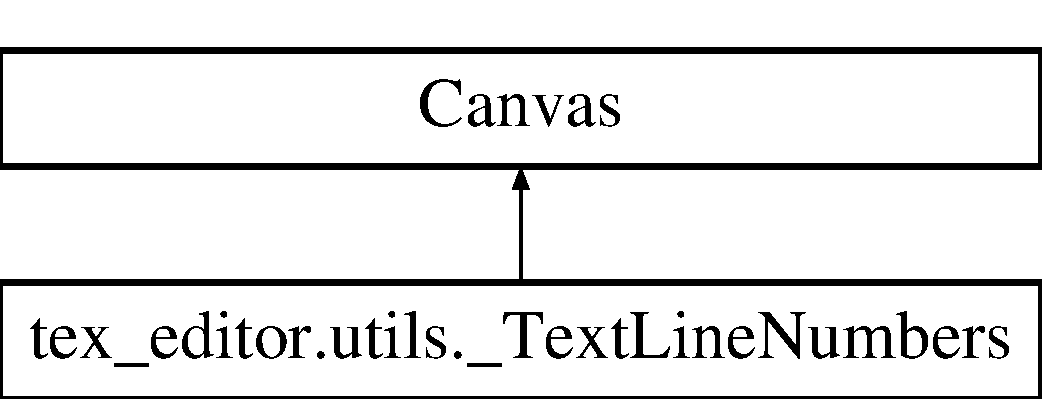
\includegraphics[height=2.000000cm]{classtex__editor_1_1utils_1_1___text_line_numbers}
\end{center}
\end{figure}
\subsection*{Fonctions membres publiques}
\begin{DoxyCompactItemize}
\item 
def \hyperlink{classtex__editor_1_1utils_1_1___text_line_numbers_af251872af54e4cf0cb4507bb2aaebfb2}{\+\_\+\+\_\+init\+\_\+\+\_\+} (self, args, kwargs)
\item 
def \hyperlink{classtex__editor_1_1utils_1_1___text_line_numbers_abe5fcdc8aa28a2506d28e31f90e55dad}{attach} (self, text\+\_\+widget)
\item 
def \hyperlink{classtex__editor_1_1utils_1_1___text_line_numbers_a791618e64f898ba331f0ede58ce4f0be}{redraw} (self, args)
\end{DoxyCompactItemize}
\subsection*{Attributs publics}
\begin{DoxyCompactItemize}
\item 
\hyperlink{classtex__editor_1_1utils_1_1___text_line_numbers_afe4b9ad6310abd726459950d1bc83882}{textwidget}
\end{DoxyCompactItemize}


\subsection{Description détaillée}
\begin{DoxyVerb}@class _TextLineNumbers

A tkinter widget that displays the line numbers of a Text zone.
It can be attached to any text widget.

@see SpecialText
\end{DoxyVerb}
 

Définition à la ligne 31 du fichier utils.\+py.



\subsection{Documentation des constructeurs et destructeur}
\hypertarget{classtex__editor_1_1utils_1_1___text_line_numbers_af251872af54e4cf0cb4507bb2aaebfb2}{}\index{tex\+\_\+editor\+::utils\+::\+\_\+\+Text\+Line\+Numbers@{tex\+\_\+editor\+::utils\+::\+\_\+\+Text\+Line\+Numbers}!\+\_\+\+\_\+init\+\_\+\+\_\+@{\+\_\+\+\_\+init\+\_\+\+\_\+}}
\index{\+\_\+\+\_\+init\+\_\+\+\_\+@{\+\_\+\+\_\+init\+\_\+\+\_\+}!tex\+\_\+editor\+::utils\+::\+\_\+\+Text\+Line\+Numbers@{tex\+\_\+editor\+::utils\+::\+\_\+\+Text\+Line\+Numbers}}
\subsubsection[{\+\_\+\+\_\+init\+\_\+\+\_\+}]{\setlength{\rightskip}{0pt plus 5cm}def tex\+\_\+editor.\+utils.\+\_\+\+Text\+Line\+Numbers.\+\_\+\+\_\+init\+\_\+\+\_\+ (
\begin{DoxyParamCaption}
\item[{}]{self, }
\item[{}]{args, }
\item[{}]{kwargs}
\end{DoxyParamCaption}
)}\label{classtex__editor_1_1utils_1_1___text_line_numbers_af251872af54e4cf0cb4507bb2aaebfb2}


Définition à la ligne 40 du fichier utils.\+py.



\subsection{Documentation des fonctions membres}
\hypertarget{classtex__editor_1_1utils_1_1___text_line_numbers_abe5fcdc8aa28a2506d28e31f90e55dad}{}\index{tex\+\_\+editor\+::utils\+::\+\_\+\+Text\+Line\+Numbers@{tex\+\_\+editor\+::utils\+::\+\_\+\+Text\+Line\+Numbers}!attach@{attach}}
\index{attach@{attach}!tex\+\_\+editor\+::utils\+::\+\_\+\+Text\+Line\+Numbers@{tex\+\_\+editor\+::utils\+::\+\_\+\+Text\+Line\+Numbers}}
\subsubsection[{attach}]{\setlength{\rightskip}{0pt plus 5cm}def tex\+\_\+editor.\+utils.\+\_\+\+Text\+Line\+Numbers.\+attach (
\begin{DoxyParamCaption}
\item[{}]{self, }
\item[{}]{text\+\_\+widget}
\end{DoxyParamCaption}
)}\label{classtex__editor_1_1utils_1_1___text_line_numbers_abe5fcdc8aa28a2506d28e31f90e55dad}


Définition à la ligne 44 du fichier utils.\+py.

\hypertarget{classtex__editor_1_1utils_1_1___text_line_numbers_a791618e64f898ba331f0ede58ce4f0be}{}\index{tex\+\_\+editor\+::utils\+::\+\_\+\+Text\+Line\+Numbers@{tex\+\_\+editor\+::utils\+::\+\_\+\+Text\+Line\+Numbers}!redraw@{redraw}}
\index{redraw@{redraw}!tex\+\_\+editor\+::utils\+::\+\_\+\+Text\+Line\+Numbers@{tex\+\_\+editor\+::utils\+::\+\_\+\+Text\+Line\+Numbers}}
\subsubsection[{redraw}]{\setlength{\rightskip}{0pt plus 5cm}def tex\+\_\+editor.\+utils.\+\_\+\+Text\+Line\+Numbers.\+redraw (
\begin{DoxyParamCaption}
\item[{}]{self, }
\item[{}]{args}
\end{DoxyParamCaption}
)}\label{classtex__editor_1_1utils_1_1___text_line_numbers_a791618e64f898ba331f0ede58ce4f0be}
\begin{DoxyVerb}Redraw line numbers.
\end{DoxyVerb}
 

Définition à la ligne 47 du fichier utils.\+py.



\subsection{Documentation des données membres}
\hypertarget{classtex__editor_1_1utils_1_1___text_line_numbers_afe4b9ad6310abd726459950d1bc83882}{}\index{tex\+\_\+editor\+::utils\+::\+\_\+\+Text\+Line\+Numbers@{tex\+\_\+editor\+::utils\+::\+\_\+\+Text\+Line\+Numbers}!textwidget@{textwidget}}
\index{textwidget@{textwidget}!tex\+\_\+editor\+::utils\+::\+\_\+\+Text\+Line\+Numbers@{tex\+\_\+editor\+::utils\+::\+\_\+\+Text\+Line\+Numbers}}
\subsubsection[{textwidget}]{\setlength{\rightskip}{0pt plus 5cm}tex\+\_\+editor.\+utils.\+\_\+\+Text\+Line\+Numbers.\+textwidget}\label{classtex__editor_1_1utils_1_1___text_line_numbers_afe4b9ad6310abd726459950d1bc83882}


Définition à la ligne 42 du fichier utils.\+py.



La documentation de cette classe a été générée à partir du fichier suivant \+:\begin{DoxyCompactItemize}
\item 
src/tex\+\_\+editor/\hyperlink{utils_8py}{utils.\+py}\end{DoxyCompactItemize}

\hypertarget{classaction__handler_1_1_action_handler}{}\section{Référence de la classe action\+\_\+handler.\+Action\+Handler}
\label{classaction__handler_1_1_action_handler}\index{action\+\_\+handler.\+Action\+Handler@{action\+\_\+handler.\+Action\+Handler}}
Graphe d\textquotesingle{}héritage de action\+\_\+handler.\+Action\+Handler\+:\begin{figure}[H]
\begin{center}
\leavevmode
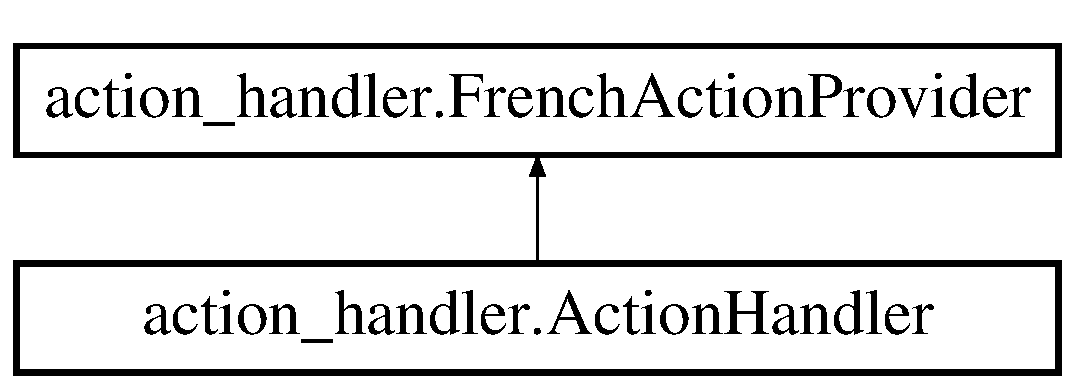
\includegraphics[height=2.000000cm]{classaction__handler_1_1_action_handler}
\end{center}
\end{figure}
\subsection*{Fonctions membres publiques}
\begin{DoxyCompactItemize}
\item 
def \hyperlink{classaction__handler_1_1_action_handler_ab9353689ea144753aa81274cfd2b3e94}{\+\_\+\+\_\+init\+\_\+\+\_\+}
\item 
def \hyperlink{classaction__handler_1_1_action_handler_a858006ca7b4e89fd9aaec7380082f27d}{get\+\_\+stringvar} (self)
\item 
def \hyperlink{classaction__handler_1_1_action_handler_a317de21aadbf2d67e94dd08e2834a88b}{on\+\_\+hit\+\_\+return\+\_\+in\+\_\+text}
\item 
def \hyperlink{classaction__handler_1_1_action_handler_a5972a9333f2409dede194e38ed84fa56}{on\+\_\+syn} (self)
\item 
def \hyperlink{classaction__handler_1_1_action_handler_a36ba2d42c8aef651793086a5ab9b24b2}{on\+\_\+ri} (self)
\item 
def \hyperlink{classaction__handler_1_1_action_handler_a03e4f47e31a72b8f88f7532471ae9aac}{on\+\_\+ct} (self, nb)
\item 
def \hyperlink{classaction__handler_1_1_action_handler_a3326e440d1af67c7f47f44e7cf495f1f}{on\+\_\+read}
\item 
def \hyperlink{classaction__handler_1_1_action_handler_ab473b0ae56991350b6668d5b654ffe97}{read} (self, begin, end)
\item 
def \hyperlink{classaction__handler_1_1_action_handler_a40f47fb4537fed9b037fe547c637316a}{on\+\_\+remove\+\_\+error\+\_\+tags}
\item 
def \hyperlink{classaction__handler_1_1_action_handler_a9a1f3c2b07ed4841cc412f7719be139d}{on\+\_\+closing} (self)
\end{DoxyCompactItemize}
\subsection*{Attributs publics}
\begin{DoxyCompactItemize}
\item 
\hyperlink{classaction__handler_1_1_action_handler_ae7daf04ab97af90c74394a2a860fcb0c}{sw}
\item 
\hyperlink{classaction__handler_1_1_action_handler_a30a752ec44884f0ec249a2222746723a}{text}
\item 
\hyperlink{classaction__handler_1_1_action_handler_a967fddb2d69abb7e13683d36d404fc29}{output}
\end{DoxyCompactItemize}


\subsection{Description détaillée}
\begin{DoxyVerb}@class ActionHandler\end{DoxyVerb}
 

Définition à la ligne 105 du fichier action\+\_\+handler.\+py.



\subsection{Documentation des constructeurs et destructeur}
\hypertarget{classaction__handler_1_1_action_handler_ab9353689ea144753aa81274cfd2b3e94}{}\index{action\+\_\+handler\+::\+Action\+Handler@{action\+\_\+handler\+::\+Action\+Handler}!\+\_\+\+\_\+init\+\_\+\+\_\+@{\+\_\+\+\_\+init\+\_\+\+\_\+}}
\index{\+\_\+\+\_\+init\+\_\+\+\_\+@{\+\_\+\+\_\+init\+\_\+\+\_\+}!action\+\_\+handler\+::\+Action\+Handler@{action\+\_\+handler\+::\+Action\+Handler}}
\subsubsection[{\+\_\+\+\_\+init\+\_\+\+\_\+}]{\setlength{\rightskip}{0pt plus 5cm}def action\+\_\+handler.\+Action\+Handler.\+\_\+\+\_\+init\+\_\+\+\_\+ (
\begin{DoxyParamCaption}
\item[{}]{self, }
\item[{}]{textzone = {\ttfamily None}, }
\item[{}]{textoutput = {\ttfamily None}}
\end{DoxyParamCaption}
)}\label{classaction__handler_1_1_action_handler_ab9353689ea144753aa81274cfd2b3e94}


Définition à la ligne 111 du fichier action\+\_\+handler.\+py.



\subsection{Documentation des fonctions membres}
\hypertarget{classaction__handler_1_1_action_handler_a858006ca7b4e89fd9aaec7380082f27d}{}\index{action\+\_\+handler\+::\+Action\+Handler@{action\+\_\+handler\+::\+Action\+Handler}!get\+\_\+stringvar@{get\+\_\+stringvar}}
\index{get\+\_\+stringvar@{get\+\_\+stringvar}!action\+\_\+handler\+::\+Action\+Handler@{action\+\_\+handler\+::\+Action\+Handler}}
\subsubsection[{get\+\_\+stringvar}]{\setlength{\rightskip}{0pt plus 5cm}def action\+\_\+handler.\+Action\+Handler.\+get\+\_\+stringvar (
\begin{DoxyParamCaption}
\item[{}]{self}
\end{DoxyParamCaption}
)}\label{classaction__handler_1_1_action_handler_a858006ca7b4e89fd9aaec7380082f27d}


Définition à la ligne 132 du fichier action\+\_\+handler.\+py.

\hypertarget{classaction__handler_1_1_action_handler_a9a1f3c2b07ed4841cc412f7719be139d}{}\index{action\+\_\+handler\+::\+Action\+Handler@{action\+\_\+handler\+::\+Action\+Handler}!on\+\_\+closing@{on\+\_\+closing}}
\index{on\+\_\+closing@{on\+\_\+closing}!action\+\_\+handler\+::\+Action\+Handler@{action\+\_\+handler\+::\+Action\+Handler}}
\subsubsection[{on\+\_\+closing}]{\setlength{\rightskip}{0pt plus 5cm}def action\+\_\+handler.\+Action\+Handler.\+on\+\_\+closing (
\begin{DoxyParamCaption}
\item[{}]{self}
\end{DoxyParamCaption}
)}\label{classaction__handler_1_1_action_handler_a9a1f3c2b07ed4841cc412f7719be139d}


Définition à la ligne 271 du fichier action\+\_\+handler.\+py.

\hypertarget{classaction__handler_1_1_action_handler_a03e4f47e31a72b8f88f7532471ae9aac}{}\index{action\+\_\+handler\+::\+Action\+Handler@{action\+\_\+handler\+::\+Action\+Handler}!on\+\_\+ct@{on\+\_\+ct}}
\index{on\+\_\+ct@{on\+\_\+ct}!action\+\_\+handler\+::\+Action\+Handler@{action\+\_\+handler\+::\+Action\+Handler}}
\subsubsection[{on\+\_\+ct}]{\setlength{\rightskip}{0pt plus 5cm}def action\+\_\+handler.\+Action\+Handler.\+on\+\_\+ct (
\begin{DoxyParamCaption}
\item[{}]{self, }
\item[{}]{nb}
\end{DoxyParamCaption}
)}\label{classaction__handler_1_1_action_handler_a03e4f47e31a72b8f88f7532471ae9aac}


Définition à la ligne 165 du fichier action\+\_\+handler.\+py.

\hypertarget{classaction__handler_1_1_action_handler_a317de21aadbf2d67e94dd08e2834a88b}{}\index{action\+\_\+handler\+::\+Action\+Handler@{action\+\_\+handler\+::\+Action\+Handler}!on\+\_\+hit\+\_\+return\+\_\+in\+\_\+text@{on\+\_\+hit\+\_\+return\+\_\+in\+\_\+text}}
\index{on\+\_\+hit\+\_\+return\+\_\+in\+\_\+text@{on\+\_\+hit\+\_\+return\+\_\+in\+\_\+text}!action\+\_\+handler\+::\+Action\+Handler@{action\+\_\+handler\+::\+Action\+Handler}}
\subsubsection[{on\+\_\+hit\+\_\+return\+\_\+in\+\_\+text}]{\setlength{\rightskip}{0pt plus 5cm}def action\+\_\+handler.\+Action\+Handler.\+on\+\_\+hit\+\_\+return\+\_\+in\+\_\+text (
\begin{DoxyParamCaption}
\item[{}]{self, }
\item[{}]{event = {\ttfamily None}}
\end{DoxyParamCaption}
)}\label{classaction__handler_1_1_action_handler_a317de21aadbf2d67e94dd08e2834a88b}


Définition à la ligne 136 du fichier action\+\_\+handler.\+py.

\hypertarget{classaction__handler_1_1_action_handler_a3326e440d1af67c7f47f44e7cf495f1f}{}\index{action\+\_\+handler\+::\+Action\+Handler@{action\+\_\+handler\+::\+Action\+Handler}!on\+\_\+read@{on\+\_\+read}}
\index{on\+\_\+read@{on\+\_\+read}!action\+\_\+handler\+::\+Action\+Handler@{action\+\_\+handler\+::\+Action\+Handler}}
\subsubsection[{on\+\_\+read}]{\setlength{\rightskip}{0pt plus 5cm}def action\+\_\+handler.\+Action\+Handler.\+on\+\_\+read (
\begin{DoxyParamCaption}
\item[{}]{self, }
\item[{}]{event = {\ttfamily None}}
\end{DoxyParamCaption}
)}\label{classaction__handler_1_1_action_handler_a3326e440d1af67c7f47f44e7cf495f1f}


Définition à la ligne 213 du fichier action\+\_\+handler.\+py.

\hypertarget{classaction__handler_1_1_action_handler_a40f47fb4537fed9b037fe547c637316a}{}\index{action\+\_\+handler\+::\+Action\+Handler@{action\+\_\+handler\+::\+Action\+Handler}!on\+\_\+remove\+\_\+error\+\_\+tags@{on\+\_\+remove\+\_\+error\+\_\+tags}}
\index{on\+\_\+remove\+\_\+error\+\_\+tags@{on\+\_\+remove\+\_\+error\+\_\+tags}!action\+\_\+handler\+::\+Action\+Handler@{action\+\_\+handler\+::\+Action\+Handler}}
\subsubsection[{on\+\_\+remove\+\_\+error\+\_\+tags}]{\setlength{\rightskip}{0pt plus 5cm}def action\+\_\+handler.\+Action\+Handler.\+on\+\_\+remove\+\_\+error\+\_\+tags (
\begin{DoxyParamCaption}
\item[{}]{self, }
\item[{}]{event = {\ttfamily None}}
\end{DoxyParamCaption}
)}\label{classaction__handler_1_1_action_handler_a40f47fb4537fed9b037fe547c637316a}


Définition à la ligne 258 du fichier action\+\_\+handler.\+py.

\hypertarget{classaction__handler_1_1_action_handler_a36ba2d42c8aef651793086a5ab9b24b2}{}\index{action\+\_\+handler\+::\+Action\+Handler@{action\+\_\+handler\+::\+Action\+Handler}!on\+\_\+ri@{on\+\_\+ri}}
\index{on\+\_\+ri@{on\+\_\+ri}!action\+\_\+handler\+::\+Action\+Handler@{action\+\_\+handler\+::\+Action\+Handler}}
\subsubsection[{on\+\_\+ri}]{\setlength{\rightskip}{0pt plus 5cm}def action\+\_\+handler.\+Action\+Handler.\+on\+\_\+ri (
\begin{DoxyParamCaption}
\item[{}]{self}
\end{DoxyParamCaption}
)}\label{classaction__handler_1_1_action_handler_a36ba2d42c8aef651793086a5ab9b24b2}


Définition à la ligne 153 du fichier action\+\_\+handler.\+py.

\hypertarget{classaction__handler_1_1_action_handler_a5972a9333f2409dede194e38ed84fa56}{}\index{action\+\_\+handler\+::\+Action\+Handler@{action\+\_\+handler\+::\+Action\+Handler}!on\+\_\+syn@{on\+\_\+syn}}
\index{on\+\_\+syn@{on\+\_\+syn}!action\+\_\+handler\+::\+Action\+Handler@{action\+\_\+handler\+::\+Action\+Handler}}
\subsubsection[{on\+\_\+syn}]{\setlength{\rightskip}{0pt plus 5cm}def action\+\_\+handler.\+Action\+Handler.\+on\+\_\+syn (
\begin{DoxyParamCaption}
\item[{}]{self}
\end{DoxyParamCaption}
)}\label{classaction__handler_1_1_action_handler_a5972a9333f2409dede194e38ed84fa56}


Définition à la ligne 141 du fichier action\+\_\+handler.\+py.

\hypertarget{classaction__handler_1_1_action_handler_ab473b0ae56991350b6668d5b654ffe97}{}\index{action\+\_\+handler\+::\+Action\+Handler@{action\+\_\+handler\+::\+Action\+Handler}!read@{read}}
\index{read@{read}!action\+\_\+handler\+::\+Action\+Handler@{action\+\_\+handler\+::\+Action\+Handler}}
\subsubsection[{read}]{\setlength{\rightskip}{0pt plus 5cm}def action\+\_\+handler.\+Action\+Handler.\+read (
\begin{DoxyParamCaption}
\item[{}]{self, }
\item[{}]{begin, }
\item[{}]{end}
\end{DoxyParamCaption}
)}\label{classaction__handler_1_1_action_handler_ab473b0ae56991350b6668d5b654ffe97}
\begin{DoxyVerb}Calls the text parser (reading and verifying) on the selection begin-end.
\end{DoxyVerb}
 

Définition à la ligne 219 du fichier action\+\_\+handler.\+py.



\subsection{Documentation des données membres}
\hypertarget{classaction__handler_1_1_action_handler_a967fddb2d69abb7e13683d36d404fc29}{}\index{action\+\_\+handler\+::\+Action\+Handler@{action\+\_\+handler\+::\+Action\+Handler}!output@{output}}
\index{output@{output}!action\+\_\+handler\+::\+Action\+Handler@{action\+\_\+handler\+::\+Action\+Handler}}
\subsubsection[{output}]{\setlength{\rightskip}{0pt plus 5cm}action\+\_\+handler.\+Action\+Handler.\+output}\label{classaction__handler_1_1_action_handler_a967fddb2d69abb7e13683d36d404fc29}


Définition à la ligne 127 du fichier action\+\_\+handler.\+py.

\hypertarget{classaction__handler_1_1_action_handler_ae7daf04ab97af90c74394a2a860fcb0c}{}\index{action\+\_\+handler\+::\+Action\+Handler@{action\+\_\+handler\+::\+Action\+Handler}!sw@{sw}}
\index{sw@{sw}!action\+\_\+handler\+::\+Action\+Handler@{action\+\_\+handler\+::\+Action\+Handler}}
\subsubsection[{sw}]{\setlength{\rightskip}{0pt plus 5cm}action\+\_\+handler.\+Action\+Handler.\+sw}\label{classaction__handler_1_1_action_handler_ae7daf04ab97af90c74394a2a860fcb0c}


Définition à la ligne 118 du fichier action\+\_\+handler.\+py.

\hypertarget{classaction__handler_1_1_action_handler_a30a752ec44884f0ec249a2222746723a}{}\index{action\+\_\+handler\+::\+Action\+Handler@{action\+\_\+handler\+::\+Action\+Handler}!text@{text}}
\index{text@{text}!action\+\_\+handler\+::\+Action\+Handler@{action\+\_\+handler\+::\+Action\+Handler}}
\subsubsection[{text}]{\setlength{\rightskip}{0pt plus 5cm}action\+\_\+handler.\+Action\+Handler.\+text}\label{classaction__handler_1_1_action_handler_a30a752ec44884f0ec249a2222746723a}


Définition à la ligne 121 du fichier action\+\_\+handler.\+py.



La documentation de cette classe a été générée à partir du fichier suivant \+:\begin{DoxyCompactItemize}
\item 
src/mainframe/\hyperlink{action__handler_8py}{action\+\_\+handler.\+py}\end{DoxyCompactItemize}

\hypertarget{classtex__editor_1_1text_1_1_button_panel}{}\section{Référence de la classe tex\+\_\+editor.\+text.\+Button\+Panel}
\label{classtex__editor_1_1text_1_1_button_panel}\index{tex\+\_\+editor.\+text.\+Button\+Panel@{tex\+\_\+editor.\+text.\+Button\+Panel}}
Graphe d\textquotesingle{}héritage de tex\+\_\+editor.\+text.\+Button\+Panel\+:\begin{figure}[H]
\begin{center}
\leavevmode
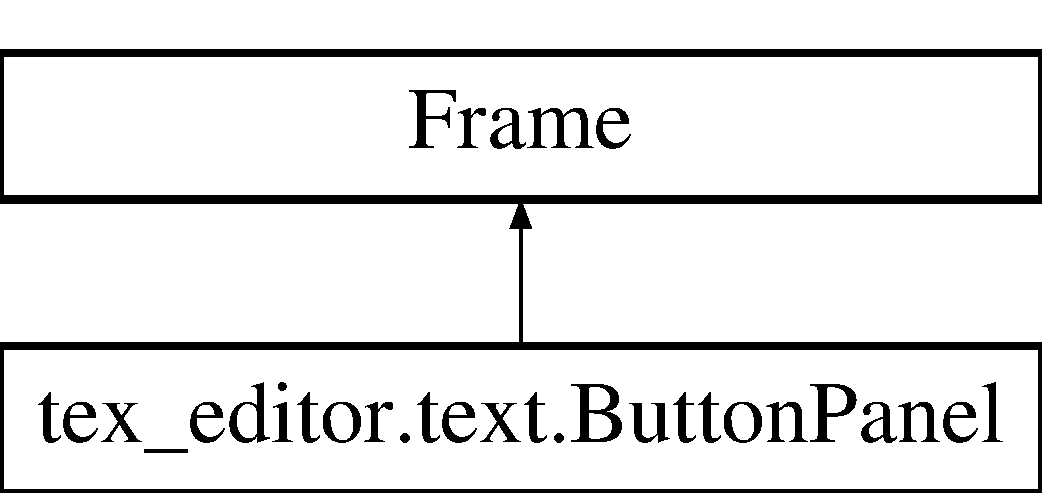
\includegraphics[height=2.000000cm]{classtex__editor_1_1text_1_1_button_panel}
\end{center}
\end{figure}
\subsection*{Fonctions membres publiques}
\begin{DoxyCompactItemize}
\item 
def \hyperlink{classtex__editor_1_1text_1_1_button_panel_a734cef760e167774b45e88297dadc1f7}{\+\_\+\+\_\+init\+\_\+\+\_\+} (self, args, kwargs)
\item 
def \hyperlink{classtex__editor_1_1text_1_1_button_panel_a3d2ba27c5be72cd6b6ada767882153f0}{attach} (self, textwidget)
\end{DoxyCompactItemize}


\subsection{Description détaillée}
\begin{DoxyVerb}@class ButtonPanel

A panel of buttons that can be attached to a text widget that is a subclass
of SpecialText (to have all the methods needed).

The formatting buttons control which tag is set and which ones automatically
removed.

@see SpecialText
\end{DoxyVerb}
 

Définition à la ligne 67 du fichier text.\+py.



\subsection{Documentation des constructeurs et destructeur}
\hypertarget{classtex__editor_1_1text_1_1_button_panel_a734cef760e167774b45e88297dadc1f7}{}\index{tex\+\_\+editor\+::text\+::\+Button\+Panel@{tex\+\_\+editor\+::text\+::\+Button\+Panel}!\+\_\+\+\_\+init\+\_\+\+\_\+@{\+\_\+\+\_\+init\+\_\+\+\_\+}}
\index{\+\_\+\+\_\+init\+\_\+\+\_\+@{\+\_\+\+\_\+init\+\_\+\+\_\+}!tex\+\_\+editor\+::text\+::\+Button\+Panel@{tex\+\_\+editor\+::text\+::\+Button\+Panel}}
\subsubsection[{\+\_\+\+\_\+init\+\_\+\+\_\+}]{\setlength{\rightskip}{0pt plus 5cm}def tex\+\_\+editor.\+text.\+Button\+Panel.\+\_\+\+\_\+init\+\_\+\+\_\+ (
\begin{DoxyParamCaption}
\item[{}]{self, }
\item[{}]{args, }
\item[{}]{kwargs}
\end{DoxyParamCaption}
)}\label{classtex__editor_1_1text_1_1_button_panel_a734cef760e167774b45e88297dadc1f7}


Définition à la ligne 80 du fichier text.\+py.



\subsection{Documentation des fonctions membres}
\hypertarget{classtex__editor_1_1text_1_1_button_panel_a3d2ba27c5be72cd6b6ada767882153f0}{}\index{tex\+\_\+editor\+::text\+::\+Button\+Panel@{tex\+\_\+editor\+::text\+::\+Button\+Panel}!attach@{attach}}
\index{attach@{attach}!tex\+\_\+editor\+::text\+::\+Button\+Panel@{tex\+\_\+editor\+::text\+::\+Button\+Panel}}
\subsubsection[{attach}]{\setlength{\rightskip}{0pt plus 5cm}def tex\+\_\+editor.\+text.\+Button\+Panel.\+attach (
\begin{DoxyParamCaption}
\item[{}]{self, }
\item[{}]{textwidget}
\end{DoxyParamCaption}
)}\label{classtex__editor_1_1text_1_1_button_panel_a3d2ba27c5be72cd6b6ada767882153f0}


Définition à la ligne 201 du fichier text.\+py.



La documentation de cette classe a été générée à partir du fichier suivant \+:\begin{DoxyCompactItemize}
\item 
src/tex\+\_\+editor/\hyperlink{text_8py}{text.\+py}\end{DoxyCompactItemize}

\hypertarget{classdata__manager_1_1_data_manager}{}\section{Référence de la classe data\+\_\+manager.\+Data\+Manager}
\label{classdata__manager_1_1_data_manager}\index{data\+\_\+manager.\+Data\+Manager@{data\+\_\+manager.\+Data\+Manager}}
\subsection*{Fonctions membres publiques}
\begin{DoxyCompactItemize}
\item 
def \hyperlink{classdata__manager_1_1_data_manager_ac366e9ff1e60bbd9f1af6f03c16786be}{\+\_\+\+\_\+init\+\_\+\+\_\+}
\item 
def \hyperlink{classdata__manager_1_1_data_manager_a0b90348fcc9ebeb7a2393765fdc75cc7}{get\+\_\+stringvar} (self)
\item 
def \hyperlink{classdata__manager_1_1_data_manager_a0e818a89edc720833d52e2fc4ccb1a31}{on\+\_\+closing} (self)
\item 
def \hyperlink{classdata__manager_1_1_data_manager_a6fde021d521f4e02dc2a4fae1e721be8}{on\+\_\+new}
\item 
def \hyperlink{classdata__manager_1_1_data_manager_a8f1069e0155969fa47d8d8e8c5da2bdd}{on\+\_\+open}
\item 
def \hyperlink{classdata__manager_1_1_data_manager_a6b949b5df5c7be9ded8b1314256df344}{on\+\_\+save}
\item 
def \hyperlink{classdata__manager_1_1_data_manager_af6bae58ad61e4562021fcd189c738589}{on\+\_\+save\+\_\+new} (self)
\item 
def \hyperlink{classdata__manager_1_1_data_manager_af9816290b2039dc26d48fc3c5990e670}{on\+\_\+export\+\_\+tex} (self)
\item 
def \hyperlink{classdata__manager_1_1_data_manager_ae4c3f0e81ad3da2ea9105576f6f2ab09}{on\+\_\+change\+\_\+count} (self)
\item 
def \hyperlink{classdata__manager_1_1_data_manager_a866ee05596fa52b5540c8db7df0034b0}{load\+\_\+params} (self)
\item 
def \hyperlink{classdata__manager_1_1_data_manager_ac3724c07fb0dba2249a906b3d9da3ba1}{save\+\_\+params} (self)
\item 
def \hyperlink{classdata__manager_1_1_data_manager_af5ad2779320a0cb48526a5b7ec2f8ace}{set\+\_\+current\+\_\+file} (self, filename)
\item 
def \hyperlink{classdata__manager_1_1_data_manager_a6d9aaaba2137be3167c4de0551c19cc1}{open\+\_\+file} (self, filename)
\item 
def \hyperlink{classdata__manager_1_1_data_manager_a18246d4222716e94d1e7fd679c10971b}{save\+\_\+to\+\_\+file} (self, filename)
\end{DoxyCompactItemize}
\subsection*{Attributs publics}
\begin{DoxyCompactItemize}
\item 
\hyperlink{classdata__manager_1_1_data_manager_afc5dea5a6cfb094c0afaa794d6a43784}{cf}
\item 
\hyperlink{classdata__manager_1_1_data_manager_a64c90baeeef1e87cd2bc08228f591be0}{text}
\item 
\hyperlink{classdata__manager_1_1_data_manager_a6f3933032672ae43ca7029531c4178ea}{params}
\end{DoxyCompactItemize}


\subsection{Description détaillée}
\begin{DoxyVerb}Attach this to a text widget to interface with the data and parameters.

The text widget must have all the methods of a TexFormattedText.
\end{DoxyVerb}
 

Définition à la ligne 18 du fichier data\+\_\+manager.\+py.



\subsection{Documentation des constructeurs et destructeur}
\hypertarget{classdata__manager_1_1_data_manager_ac366e9ff1e60bbd9f1af6f03c16786be}{}\index{data\+\_\+manager\+::\+Data\+Manager@{data\+\_\+manager\+::\+Data\+Manager}!\+\_\+\+\_\+init\+\_\+\+\_\+@{\+\_\+\+\_\+init\+\_\+\+\_\+}}
\index{\+\_\+\+\_\+init\+\_\+\+\_\+@{\+\_\+\+\_\+init\+\_\+\+\_\+}!data\+\_\+manager\+::\+Data\+Manager@{data\+\_\+manager\+::\+Data\+Manager}}
\subsubsection[{\+\_\+\+\_\+init\+\_\+\+\_\+}]{\setlength{\rightskip}{0pt plus 5cm}def data\+\_\+manager.\+Data\+Manager.\+\_\+\+\_\+init\+\_\+\+\_\+ (
\begin{DoxyParamCaption}
\item[{}]{self, }
\item[{}]{textzone = {\ttfamily None}}
\end{DoxyParamCaption}
)}\label{classdata__manager_1_1_data_manager_ac366e9ff1e60bbd9f1af6f03c16786be}
\begin{DoxyVerb}Loads parameters and the current file to the textzone
that it is attached to.
\end{DoxyVerb}
 

Définition à la ligne 25 du fichier data\+\_\+manager.\+py.



\subsection{Documentation des fonctions membres}
\hypertarget{classdata__manager_1_1_data_manager_a0b90348fcc9ebeb7a2393765fdc75cc7}{}\index{data\+\_\+manager\+::\+Data\+Manager@{data\+\_\+manager\+::\+Data\+Manager}!get\+\_\+stringvar@{get\+\_\+stringvar}}
\index{get\+\_\+stringvar@{get\+\_\+stringvar}!data\+\_\+manager\+::\+Data\+Manager@{data\+\_\+manager\+::\+Data\+Manager}}
\subsubsection[{get\+\_\+stringvar}]{\setlength{\rightskip}{0pt plus 5cm}def data\+\_\+manager.\+Data\+Manager.\+get\+\_\+stringvar (
\begin{DoxyParamCaption}
\item[{}]{self}
\end{DoxyParamCaption}
)}\label{classdata__manager_1_1_data_manager_a0b90348fcc9ebeb7a2393765fdc75cc7}
\begin{DoxyVerb}Gets a StringVar of the current behavior of the manager.
\end{DoxyVerb}
 

Définition à la ligne 39 du fichier data\+\_\+manager.\+py.

\hypertarget{classdata__manager_1_1_data_manager_a866ee05596fa52b5540c8db7df0034b0}{}\index{data\+\_\+manager\+::\+Data\+Manager@{data\+\_\+manager\+::\+Data\+Manager}!load\+\_\+params@{load\+\_\+params}}
\index{load\+\_\+params@{load\+\_\+params}!data\+\_\+manager\+::\+Data\+Manager@{data\+\_\+manager\+::\+Data\+Manager}}
\subsubsection[{load\+\_\+params}]{\setlength{\rightskip}{0pt plus 5cm}def data\+\_\+manager.\+Data\+Manager.\+load\+\_\+params (
\begin{DoxyParamCaption}
\item[{}]{self}
\end{DoxyParamCaption}
)}\label{classdata__manager_1_1_data_manager_a866ee05596fa52b5540c8db7df0034b0}
\begin{DoxyVerb}Loads the parameters JSON file.
\end{DoxyVerb}
 

Définition à la ligne 147 du fichier data\+\_\+manager.\+py.

\hypertarget{classdata__manager_1_1_data_manager_ae4c3f0e81ad3da2ea9105576f6f2ab09}{}\index{data\+\_\+manager\+::\+Data\+Manager@{data\+\_\+manager\+::\+Data\+Manager}!on\+\_\+change\+\_\+count@{on\+\_\+change\+\_\+count}}
\index{on\+\_\+change\+\_\+count@{on\+\_\+change\+\_\+count}!data\+\_\+manager\+::\+Data\+Manager@{data\+\_\+manager\+::\+Data\+Manager}}
\subsubsection[{on\+\_\+change\+\_\+count}]{\setlength{\rightskip}{0pt plus 5cm}def data\+\_\+manager.\+Data\+Manager.\+on\+\_\+change\+\_\+count (
\begin{DoxyParamCaption}
\item[{}]{self}
\end{DoxyParamCaption}
)}\label{classdata__manager_1_1_data_manager_ae4c3f0e81ad3da2ea9105576f6f2ab09}
\begin{DoxyVerb}Change the parameter regarding verse count.
\end{DoxyVerb}
 

Définition à la ligne 132 du fichier data\+\_\+manager.\+py.

\hypertarget{classdata__manager_1_1_data_manager_a0e818a89edc720833d52e2fc4ccb1a31}{}\index{data\+\_\+manager\+::\+Data\+Manager@{data\+\_\+manager\+::\+Data\+Manager}!on\+\_\+closing@{on\+\_\+closing}}
\index{on\+\_\+closing@{on\+\_\+closing}!data\+\_\+manager\+::\+Data\+Manager@{data\+\_\+manager\+::\+Data\+Manager}}
\subsubsection[{on\+\_\+closing}]{\setlength{\rightskip}{0pt plus 5cm}def data\+\_\+manager.\+Data\+Manager.\+on\+\_\+closing (
\begin{DoxyParamCaption}
\item[{}]{self}
\end{DoxyParamCaption}
)}\label{classdata__manager_1_1_data_manager_a0e818a89edc720833d52e2fc4ccb1a31}
\begin{DoxyVerb}On closing, ask if the data must be saved.
\end{DoxyVerb}
 

Définition à la ligne 45 du fichier data\+\_\+manager.\+py.

\hypertarget{classdata__manager_1_1_data_manager_af9816290b2039dc26d48fc3c5990e670}{}\index{data\+\_\+manager\+::\+Data\+Manager@{data\+\_\+manager\+::\+Data\+Manager}!on\+\_\+export\+\_\+tex@{on\+\_\+export\+\_\+tex}}
\index{on\+\_\+export\+\_\+tex@{on\+\_\+export\+\_\+tex}!data\+\_\+manager\+::\+Data\+Manager@{data\+\_\+manager\+::\+Data\+Manager}}
\subsubsection[{on\+\_\+export\+\_\+tex}]{\setlength{\rightskip}{0pt plus 5cm}def data\+\_\+manager.\+Data\+Manager.\+on\+\_\+export\+\_\+tex (
\begin{DoxyParamCaption}
\item[{}]{self}
\end{DoxyParamCaption}
)}\label{classdata__manager_1_1_data_manager_af9816290b2039dc26d48fc3c5990e670}
\begin{DoxyVerb}Exports the contents of the text zone as a TeX file.
\end{DoxyVerb}
 

Définition à la ligne 116 du fichier data\+\_\+manager.\+py.

\hypertarget{classdata__manager_1_1_data_manager_a6fde021d521f4e02dc2a4fae1e721be8}{}\index{data\+\_\+manager\+::\+Data\+Manager@{data\+\_\+manager\+::\+Data\+Manager}!on\+\_\+new@{on\+\_\+new}}
\index{on\+\_\+new@{on\+\_\+new}!data\+\_\+manager\+::\+Data\+Manager@{data\+\_\+manager\+::\+Data\+Manager}}
\subsubsection[{on\+\_\+new}]{\setlength{\rightskip}{0pt plus 5cm}def data\+\_\+manager.\+Data\+Manager.\+on\+\_\+new (
\begin{DoxyParamCaption}
\item[{}]{self, }
\item[{}]{event = {\ttfamily None}}
\end{DoxyParamCaption}
)}\label{classdata__manager_1_1_data_manager_a6fde021d521f4e02dc2a4fae1e721be8}
\begin{DoxyVerb}When a new file is created, ask if the data must be saved.
Then delete all the contents.
\end{DoxyVerb}
 

Définition à la ligne 58 du fichier data\+\_\+manager.\+py.

\hypertarget{classdata__manager_1_1_data_manager_a8f1069e0155969fa47d8d8e8c5da2bdd}{}\index{data\+\_\+manager\+::\+Data\+Manager@{data\+\_\+manager\+::\+Data\+Manager}!on\+\_\+open@{on\+\_\+open}}
\index{on\+\_\+open@{on\+\_\+open}!data\+\_\+manager\+::\+Data\+Manager@{data\+\_\+manager\+::\+Data\+Manager}}
\subsubsection[{on\+\_\+open}]{\setlength{\rightskip}{0pt plus 5cm}def data\+\_\+manager.\+Data\+Manager.\+on\+\_\+open (
\begin{DoxyParamCaption}
\item[{}]{self, }
\item[{}]{event = {\ttfamily None}}
\end{DoxyParamCaption}
)}\label{classdata__manager_1_1_data_manager_a8f1069e0155969fa47d8d8e8c5da2bdd}
\begin{DoxyVerb}When asking to open a new file, ask if the data must be saved.
Then delete all the contents.
\end{DoxyVerb}
 

Définition à la ligne 71 du fichier data\+\_\+manager.\+py.

\hypertarget{classdata__manager_1_1_data_manager_a6b949b5df5c7be9ded8b1314256df344}{}\index{data\+\_\+manager\+::\+Data\+Manager@{data\+\_\+manager\+::\+Data\+Manager}!on\+\_\+save@{on\+\_\+save}}
\index{on\+\_\+save@{on\+\_\+save}!data\+\_\+manager\+::\+Data\+Manager@{data\+\_\+manager\+::\+Data\+Manager}}
\subsubsection[{on\+\_\+save}]{\setlength{\rightskip}{0pt plus 5cm}def data\+\_\+manager.\+Data\+Manager.\+on\+\_\+save (
\begin{DoxyParamCaption}
\item[{}]{self, }
\item[{}]{event = {\ttfamily None}}
\end{DoxyParamCaption}
)}\label{classdata__manager_1_1_data_manager_a6b949b5df5c7be9ded8b1314256df344}
\begin{DoxyVerb}Save the current file.
\end{DoxyVerb}
 

Définition à la ligne 92 du fichier data\+\_\+manager.\+py.

\hypertarget{classdata__manager_1_1_data_manager_af6bae58ad61e4562021fcd189c738589}{}\index{data\+\_\+manager\+::\+Data\+Manager@{data\+\_\+manager\+::\+Data\+Manager}!on\+\_\+save\+\_\+new@{on\+\_\+save\+\_\+new}}
\index{on\+\_\+save\+\_\+new@{on\+\_\+save\+\_\+new}!data\+\_\+manager\+::\+Data\+Manager@{data\+\_\+manager\+::\+Data\+Manager}}
\subsubsection[{on\+\_\+save\+\_\+new}]{\setlength{\rightskip}{0pt plus 5cm}def data\+\_\+manager.\+Data\+Manager.\+on\+\_\+save\+\_\+new (
\begin{DoxyParamCaption}
\item[{}]{self}
\end{DoxyParamCaption}
)}\label{classdata__manager_1_1_data_manager_af6bae58ad61e4562021fcd189c738589}
\begin{DoxyVerb}Save to a new file. First asks for this file, then
created it and sets the current file to this file.
\end{DoxyVerb}
 

Définition à la ligne 101 du fichier data\+\_\+manager.\+py.

\hypertarget{classdata__manager_1_1_data_manager_a6d9aaaba2137be3167c4de0551c19cc1}{}\index{data\+\_\+manager\+::\+Data\+Manager@{data\+\_\+manager\+::\+Data\+Manager}!open\+\_\+file@{open\+\_\+file}}
\index{open\+\_\+file@{open\+\_\+file}!data\+\_\+manager\+::\+Data\+Manager@{data\+\_\+manager\+::\+Data\+Manager}}
\subsubsection[{open\+\_\+file}]{\setlength{\rightskip}{0pt plus 5cm}def data\+\_\+manager.\+Data\+Manager.\+open\+\_\+file (
\begin{DoxyParamCaption}
\item[{}]{self, }
\item[{}]{filename}
\end{DoxyParamCaption}
)}\label{classdata__manager_1_1_data_manager_a6d9aaaba2137be3167c4de0551c19cc1}
\begin{DoxyVerb}Opens a file.
\end{DoxyVerb}
 

Définition à la ligne 195 du fichier data\+\_\+manager.\+py.

\hypertarget{classdata__manager_1_1_data_manager_ac3724c07fb0dba2249a906b3d9da3ba1}{}\index{data\+\_\+manager\+::\+Data\+Manager@{data\+\_\+manager\+::\+Data\+Manager}!save\+\_\+params@{save\+\_\+params}}
\index{save\+\_\+params@{save\+\_\+params}!data\+\_\+manager\+::\+Data\+Manager@{data\+\_\+manager\+::\+Data\+Manager}}
\subsubsection[{save\+\_\+params}]{\setlength{\rightskip}{0pt plus 5cm}def data\+\_\+manager.\+Data\+Manager.\+save\+\_\+params (
\begin{DoxyParamCaption}
\item[{}]{self}
\end{DoxyParamCaption}
)}\label{classdata__manager_1_1_data_manager_ac3724c07fb0dba2249a906b3d9da3ba1}
\begin{DoxyVerb}Saves the parameters JSON file.
\end{DoxyVerb}
 

Définition à la ligne 167 du fichier data\+\_\+manager.\+py.

\hypertarget{classdata__manager_1_1_data_manager_a18246d4222716e94d1e7fd679c10971b}{}\index{data\+\_\+manager\+::\+Data\+Manager@{data\+\_\+manager\+::\+Data\+Manager}!save\+\_\+to\+\_\+file@{save\+\_\+to\+\_\+file}}
\index{save\+\_\+to\+\_\+file@{save\+\_\+to\+\_\+file}!data\+\_\+manager\+::\+Data\+Manager@{data\+\_\+manager\+::\+Data\+Manager}}
\subsubsection[{save\+\_\+to\+\_\+file}]{\setlength{\rightskip}{0pt plus 5cm}def data\+\_\+manager.\+Data\+Manager.\+save\+\_\+to\+\_\+file (
\begin{DoxyParamCaption}
\item[{}]{self, }
\item[{}]{filename}
\end{DoxyParamCaption}
)}\label{classdata__manager_1_1_data_manager_a18246d4222716e94d1e7fd679c10971b}
\begin{DoxyVerb}Saves to a file.
\end{DoxyVerb}
 

Définition à la ligne 210 du fichier data\+\_\+manager.\+py.

\hypertarget{classdata__manager_1_1_data_manager_af5ad2779320a0cb48526a5b7ec2f8ace}{}\index{data\+\_\+manager\+::\+Data\+Manager@{data\+\_\+manager\+::\+Data\+Manager}!set\+\_\+current\+\_\+file@{set\+\_\+current\+\_\+file}}
\index{set\+\_\+current\+\_\+file@{set\+\_\+current\+\_\+file}!data\+\_\+manager\+::\+Data\+Manager@{data\+\_\+manager\+::\+Data\+Manager}}
\subsubsection[{set\+\_\+current\+\_\+file}]{\setlength{\rightskip}{0pt plus 5cm}def data\+\_\+manager.\+Data\+Manager.\+set\+\_\+current\+\_\+file (
\begin{DoxyParamCaption}
\item[{}]{self, }
\item[{}]{filename}
\end{DoxyParamCaption}
)}\label{classdata__manager_1_1_data_manager_af5ad2779320a0cb48526a5b7ec2f8ace}
\begin{DoxyVerb}Sets the current file (no file operation whatsoever here),
only parameters and labels updating.
\end{DoxyVerb}
 

Définition à la ligne 182 du fichier data\+\_\+manager.\+py.



\subsection{Documentation des données membres}
\hypertarget{classdata__manager_1_1_data_manager_afc5dea5a6cfb094c0afaa794d6a43784}{}\index{data\+\_\+manager\+::\+Data\+Manager@{data\+\_\+manager\+::\+Data\+Manager}!cf@{cf}}
\index{cf@{cf}!data\+\_\+manager\+::\+Data\+Manager@{data\+\_\+manager\+::\+Data\+Manager}}
\subsubsection[{cf}]{\setlength{\rightskip}{0pt plus 5cm}data\+\_\+manager.\+Data\+Manager.\+cf}\label{classdata__manager_1_1_data_manager_afc5dea5a6cfb094c0afaa794d6a43784}


Définition à la ligne 30 du fichier data\+\_\+manager.\+py.

\hypertarget{classdata__manager_1_1_data_manager_a6f3933032672ae43ca7029531c4178ea}{}\index{data\+\_\+manager\+::\+Data\+Manager@{data\+\_\+manager\+::\+Data\+Manager}!params@{params}}
\index{params@{params}!data\+\_\+manager\+::\+Data\+Manager@{data\+\_\+manager\+::\+Data\+Manager}}
\subsubsection[{params}]{\setlength{\rightskip}{0pt plus 5cm}data\+\_\+manager.\+Data\+Manager.\+params}\label{classdata__manager_1_1_data_manager_a6f3933032672ae43ca7029531c4178ea}


Définition à la ligne 151 du fichier data\+\_\+manager.\+py.

\hypertarget{classdata__manager_1_1_data_manager_a64c90baeeef1e87cd2bc08228f591be0}{}\index{data\+\_\+manager\+::\+Data\+Manager@{data\+\_\+manager\+::\+Data\+Manager}!text@{text}}
\index{text@{text}!data\+\_\+manager\+::\+Data\+Manager@{data\+\_\+manager\+::\+Data\+Manager}}
\subsubsection[{text}]{\setlength{\rightskip}{0pt plus 5cm}data\+\_\+manager.\+Data\+Manager.\+text}\label{classdata__manager_1_1_data_manager_a64c90baeeef1e87cd2bc08228f591be0}


Définition à la ligne 33 du fichier data\+\_\+manager.\+py.



La documentation de cette classe a été générée à partir du fichier suivant \+:\begin{DoxyCompactItemize}
\item 
src/mainframe/\hyperlink{data__manager_8py}{data\+\_\+manager.\+py}\end{DoxyCompactItemize}

\hypertarget{classaction__handler_1_1_french_action_provider}{}\section{Référence de la classe action\+\_\+handler.\+French\+Action\+Provider}
\label{classaction__handler_1_1_french_action_provider}\index{action\+\_\+handler.\+French\+Action\+Provider@{action\+\_\+handler.\+French\+Action\+Provider}}
Graphe d\textquotesingle{}héritage de action\+\_\+handler.\+French\+Action\+Provider\+:\begin{figure}[H]
\begin{center}
\leavevmode
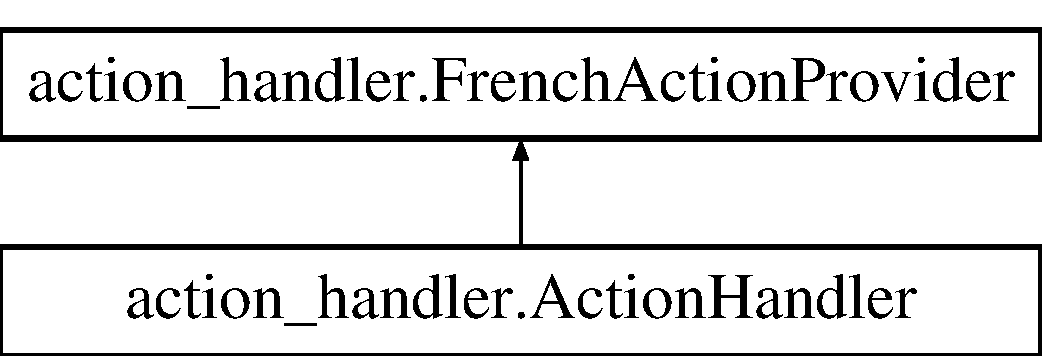
\includegraphics[height=2.000000cm]{classaction__handler_1_1_french_action_provider}
\end{center}
\end{figure}
\subsection*{Fonctions membres publiques}
\begin{DoxyCompactItemize}
\item 
def \hyperlink{classaction__handler_1_1_french_action_provider_a52e8f6c46f3e5ee688e6ddca207be4f2}{\+\_\+\+\_\+init\+\_\+\+\_\+} (self)
\item 
def \hyperlink{classaction__handler_1_1_french_action_provider_aa3ba3910751f9e706fa6e0244e89bd7b}{on\+\_\+closing} (self)
\item 
def \hyperlink{classaction__handler_1_1_french_action_provider_adf30161ac1efb5b203ba60a106c6bbc3}{get\+\_\+syns} (self, word)
\item 
def \hyperlink{classaction__handler_1_1_french_action_provider_a2abf94c2760e6855cde9c721680094c2}{get\+\_\+poor\+\_\+rimes} (self, word)
\item 
def \hyperlink{classaction__handler_1_1_french_action_provider_a2e813bf6fd1b110da8be8da47f966a23}{get\+\_\+rich\+\_\+rimes} (self, word)
\item 
def \hyperlink{classaction__handler_1_1_french_action_provider_a5fd86eb57a9312e8fa50f97f667da4b3}{get\+\_\+rimes} (self, word)
\item 
def \hyperlink{classaction__handler_1_1_french_action_provider_aee3f99571d3e6ac07f28eb39fc3cdeb7}{text\+\_\+parse} (self, text)
\item 
def \hyperlink{classaction__handler_1_1_french_action_provider_a283b0319dda1e8f63fcbd2cd6d2ce6f3}{verse\+\_\+parse} (self, text, nb)
\item 
def \hyperlink{classaction__handler_1_1_french_action_provider_ad6533993471604b01b18782f58c1fe0d}{register\+\_\+errors} (self, textw)
\end{DoxyCompactItemize}
\subsection*{Attributs publics}
\begin{DoxyCompactItemize}
\item 
\hyperlink{classaction__handler_1_1_french_action_provider_a17dc00d7d0e2f5f63963a0156ccca8c7}{connection}
\end{DoxyCompactItemize}


\subsection{Description détaillée}


Définition à la ligne 34 du fichier action\+\_\+handler.\+py.



\subsection{Documentation des constructeurs et destructeur}
\hypertarget{classaction__handler_1_1_french_action_provider_a52e8f6c46f3e5ee688e6ddca207be4f2}{}\index{action\+\_\+handler\+::\+French\+Action\+Provider@{action\+\_\+handler\+::\+French\+Action\+Provider}!\+\_\+\+\_\+init\+\_\+\+\_\+@{\+\_\+\+\_\+init\+\_\+\+\_\+}}
\index{\+\_\+\+\_\+init\+\_\+\+\_\+@{\+\_\+\+\_\+init\+\_\+\+\_\+}!action\+\_\+handler\+::\+French\+Action\+Provider@{action\+\_\+handler\+::\+French\+Action\+Provider}}
\subsubsection[{\+\_\+\+\_\+init\+\_\+\+\_\+}]{\setlength{\rightskip}{0pt plus 5cm}def action\+\_\+handler.\+French\+Action\+Provider.\+\_\+\+\_\+init\+\_\+\+\_\+ (
\begin{DoxyParamCaption}
\item[{}]{self}
\end{DoxyParamCaption}
)}\label{classaction__handler_1_1_french_action_provider_a52e8f6c46f3e5ee688e6ddca207be4f2}


Définition à la ligne 36 du fichier action\+\_\+handler.\+py.



\subsection{Documentation des fonctions membres}
\hypertarget{classaction__handler_1_1_french_action_provider_a2abf94c2760e6855cde9c721680094c2}{}\index{action\+\_\+handler\+::\+French\+Action\+Provider@{action\+\_\+handler\+::\+French\+Action\+Provider}!get\+\_\+poor\+\_\+rimes@{get\+\_\+poor\+\_\+rimes}}
\index{get\+\_\+poor\+\_\+rimes@{get\+\_\+poor\+\_\+rimes}!action\+\_\+handler\+::\+French\+Action\+Provider@{action\+\_\+handler\+::\+French\+Action\+Provider}}
\subsubsection[{get\+\_\+poor\+\_\+rimes}]{\setlength{\rightskip}{0pt plus 5cm}def action\+\_\+handler.\+French\+Action\+Provider.\+get\+\_\+poor\+\_\+rimes (
\begin{DoxyParamCaption}
\item[{}]{self, }
\item[{}]{word}
\end{DoxyParamCaption}
)}\label{classaction__handler_1_1_french_action_provider_a2abf94c2760e6855cde9c721680094c2}


Définition à la ligne 47 du fichier action\+\_\+handler.\+py.

\hypertarget{classaction__handler_1_1_french_action_provider_a2e813bf6fd1b110da8be8da47f966a23}{}\index{action\+\_\+handler\+::\+French\+Action\+Provider@{action\+\_\+handler\+::\+French\+Action\+Provider}!get\+\_\+rich\+\_\+rimes@{get\+\_\+rich\+\_\+rimes}}
\index{get\+\_\+rich\+\_\+rimes@{get\+\_\+rich\+\_\+rimes}!action\+\_\+handler\+::\+French\+Action\+Provider@{action\+\_\+handler\+::\+French\+Action\+Provider}}
\subsubsection[{get\+\_\+rich\+\_\+rimes}]{\setlength{\rightskip}{0pt plus 5cm}def action\+\_\+handler.\+French\+Action\+Provider.\+get\+\_\+rich\+\_\+rimes (
\begin{DoxyParamCaption}
\item[{}]{self, }
\item[{}]{word}
\end{DoxyParamCaption}
)}\label{classaction__handler_1_1_french_action_provider_a2e813bf6fd1b110da8be8da47f966a23}


Définition à la ligne 50 du fichier action\+\_\+handler.\+py.

\hypertarget{classaction__handler_1_1_french_action_provider_a5fd86eb57a9312e8fa50f97f667da4b3}{}\index{action\+\_\+handler\+::\+French\+Action\+Provider@{action\+\_\+handler\+::\+French\+Action\+Provider}!get\+\_\+rimes@{get\+\_\+rimes}}
\index{get\+\_\+rimes@{get\+\_\+rimes}!action\+\_\+handler\+::\+French\+Action\+Provider@{action\+\_\+handler\+::\+French\+Action\+Provider}}
\subsubsection[{get\+\_\+rimes}]{\setlength{\rightskip}{0pt plus 5cm}def action\+\_\+handler.\+French\+Action\+Provider.\+get\+\_\+rimes (
\begin{DoxyParamCaption}
\item[{}]{self, }
\item[{}]{word}
\end{DoxyParamCaption}
)}\label{classaction__handler_1_1_french_action_provider_a5fd86eb57a9312e8fa50f97f667da4b3}


Définition à la ligne 53 du fichier action\+\_\+handler.\+py.

\hypertarget{classaction__handler_1_1_french_action_provider_adf30161ac1efb5b203ba60a106c6bbc3}{}\index{action\+\_\+handler\+::\+French\+Action\+Provider@{action\+\_\+handler\+::\+French\+Action\+Provider}!get\+\_\+syns@{get\+\_\+syns}}
\index{get\+\_\+syns@{get\+\_\+syns}!action\+\_\+handler\+::\+French\+Action\+Provider@{action\+\_\+handler\+::\+French\+Action\+Provider}}
\subsubsection[{get\+\_\+syns}]{\setlength{\rightskip}{0pt plus 5cm}def action\+\_\+handler.\+French\+Action\+Provider.\+get\+\_\+syns (
\begin{DoxyParamCaption}
\item[{}]{self, }
\item[{}]{word}
\end{DoxyParamCaption}
)}\label{classaction__handler_1_1_french_action_provider_adf30161ac1efb5b203ba60a106c6bbc3}


Définition à la ligne 44 du fichier action\+\_\+handler.\+py.

\hypertarget{classaction__handler_1_1_french_action_provider_aa3ba3910751f9e706fa6e0244e89bd7b}{}\index{action\+\_\+handler\+::\+French\+Action\+Provider@{action\+\_\+handler\+::\+French\+Action\+Provider}!on\+\_\+closing@{on\+\_\+closing}}
\index{on\+\_\+closing@{on\+\_\+closing}!action\+\_\+handler\+::\+French\+Action\+Provider@{action\+\_\+handler\+::\+French\+Action\+Provider}}
\subsubsection[{on\+\_\+closing}]{\setlength{\rightskip}{0pt plus 5cm}def action\+\_\+handler.\+French\+Action\+Provider.\+on\+\_\+closing (
\begin{DoxyParamCaption}
\item[{}]{self}
\end{DoxyParamCaption}
)}\label{classaction__handler_1_1_french_action_provider_aa3ba3910751f9e706fa6e0244e89bd7b}


Définition à la ligne 40 du fichier action\+\_\+handler.\+py.

\hypertarget{classaction__handler_1_1_french_action_provider_ad6533993471604b01b18782f58c1fe0d}{}\index{action\+\_\+handler\+::\+French\+Action\+Provider@{action\+\_\+handler\+::\+French\+Action\+Provider}!register\+\_\+errors@{register\+\_\+errors}}
\index{register\+\_\+errors@{register\+\_\+errors}!action\+\_\+handler\+::\+French\+Action\+Provider@{action\+\_\+handler\+::\+French\+Action\+Provider}}
\subsubsection[{register\+\_\+errors}]{\setlength{\rightskip}{0pt plus 5cm}def action\+\_\+handler.\+French\+Action\+Provider.\+register\+\_\+errors (
\begin{DoxyParamCaption}
\item[{}]{self, }
\item[{}]{textw}
\end{DoxyParamCaption}
)}\label{classaction__handler_1_1_french_action_provider_ad6533993471604b01b18782f58c1fe0d}


Définition à la ligne 66 du fichier action\+\_\+handler.\+py.

\hypertarget{classaction__handler_1_1_french_action_provider_aee3f99571d3e6ac07f28eb39fc3cdeb7}{}\index{action\+\_\+handler\+::\+French\+Action\+Provider@{action\+\_\+handler\+::\+French\+Action\+Provider}!text\+\_\+parse@{text\+\_\+parse}}
\index{text\+\_\+parse@{text\+\_\+parse}!action\+\_\+handler\+::\+French\+Action\+Provider@{action\+\_\+handler\+::\+French\+Action\+Provider}}
\subsubsection[{text\+\_\+parse}]{\setlength{\rightskip}{0pt plus 5cm}def action\+\_\+handler.\+French\+Action\+Provider.\+text\+\_\+parse (
\begin{DoxyParamCaption}
\item[{}]{self, }
\item[{}]{text}
\end{DoxyParamCaption}
)}\label{classaction__handler_1_1_french_action_provider_aee3f99571d3e6ac07f28eb39fc3cdeb7}


Définition à la ligne 60 du fichier action\+\_\+handler.\+py.

\hypertarget{classaction__handler_1_1_french_action_provider_a283b0319dda1e8f63fcbd2cd6d2ce6f3}{}\index{action\+\_\+handler\+::\+French\+Action\+Provider@{action\+\_\+handler\+::\+French\+Action\+Provider}!verse\+\_\+parse@{verse\+\_\+parse}}
\index{verse\+\_\+parse@{verse\+\_\+parse}!action\+\_\+handler\+::\+French\+Action\+Provider@{action\+\_\+handler\+::\+French\+Action\+Provider}}
\subsubsection[{verse\+\_\+parse}]{\setlength{\rightskip}{0pt plus 5cm}def action\+\_\+handler.\+French\+Action\+Provider.\+verse\+\_\+parse (
\begin{DoxyParamCaption}
\item[{}]{self, }
\item[{}]{text, }
\item[{}]{nb}
\end{DoxyParamCaption}
)}\label{classaction__handler_1_1_french_action_provider_a283b0319dda1e8f63fcbd2cd6d2ce6f3}


Définition à la ligne 63 du fichier action\+\_\+handler.\+py.



\subsection{Documentation des données membres}
\hypertarget{classaction__handler_1_1_french_action_provider_a17dc00d7d0e2f5f63963a0156ccca8c7}{}\index{action\+\_\+handler\+::\+French\+Action\+Provider@{action\+\_\+handler\+::\+French\+Action\+Provider}!connection@{connection}}
\index{connection@{connection}!action\+\_\+handler\+::\+French\+Action\+Provider@{action\+\_\+handler\+::\+French\+Action\+Provider}}
\subsubsection[{connection}]{\setlength{\rightskip}{0pt plus 5cm}action\+\_\+handler.\+French\+Action\+Provider.\+connection}\label{classaction__handler_1_1_french_action_provider_a17dc00d7d0e2f5f63963a0156ccca8c7}


Définition à la ligne 38 du fichier action\+\_\+handler.\+py.



La documentation de cette classe a été générée à partir du fichier suivant \+:\begin{DoxyCompactItemize}
\item 
src/mainframe/\hyperlink{action__handler_8py}{action\+\_\+handler.\+py}\end{DoxyCompactItemize}

\hypertarget{classmainframe_1_1_main_frame}{}\section{Référence de la classe mainframe.\+Main\+Frame}
\label{classmainframe_1_1_main_frame}\index{mainframe.\+Main\+Frame@{mainframe.\+Main\+Frame}}
Graphe d\textquotesingle{}héritage de mainframe.\+Main\+Frame\+:\begin{figure}[H]
\begin{center}
\leavevmode
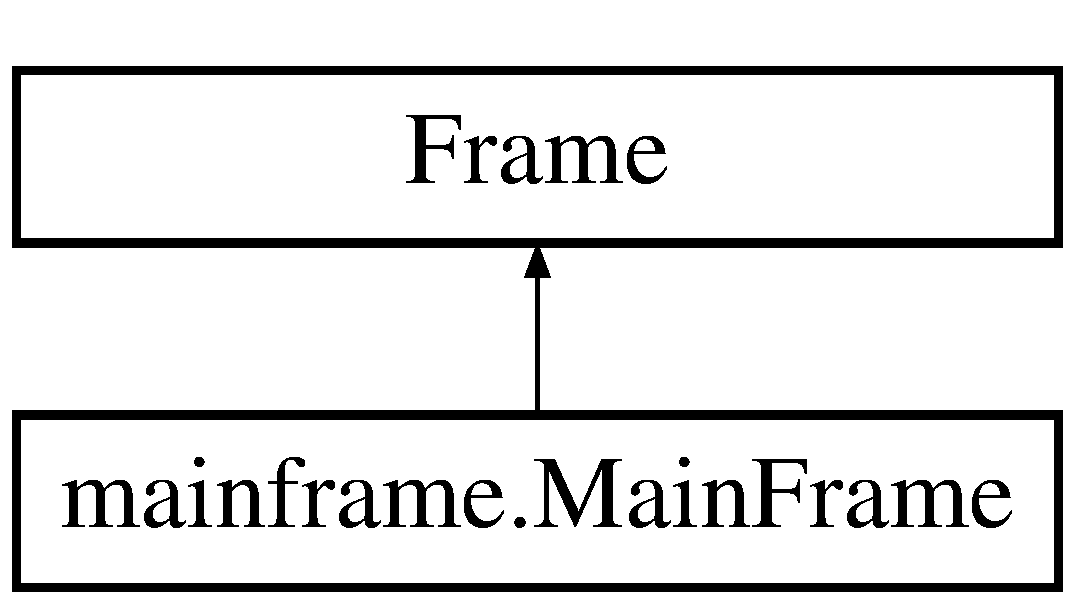
\includegraphics[height=2.000000cm]{classmainframe_1_1_main_frame}
\end{center}
\end{figure}
\subsection*{Fonctions membres publiques}
\begin{DoxyCompactItemize}
\item 
def \hyperlink{classmainframe_1_1_main_frame_ae273e00e7ef8318148092db1fbd31630}{\+\_\+\+\_\+init\+\_\+\+\_\+}
\item 
def \hyperlink{classmainframe_1_1_main_frame_a2756420d261b48a5b9136150f16d2c78}{on\+\_\+closing}
\end{DoxyCompactItemize}
\subsection*{Attributs publics}
\begin{DoxyCompactItemize}
\item 
\hyperlink{classmainframe_1_1_main_frame_af1af1736f4265c359d01ed94192f5be2}{text}
\item 
\hyperlink{classmainframe_1_1_main_frame_a0efaec7fc32e3ba7fd3bbf5091d00610}{output}
\item 
\hyperlink{classmainframe_1_1_main_frame_af7330830e57d05409e91fd989cbbcc5d}{action\+\_\+handler}
\item 
\hyperlink{classmainframe_1_1_main_frame_a2ea855c763e8591d4a828656f75ef6f1}{data\+\_\+manager}
\item 
\hyperlink{classmainframe_1_1_main_frame_adb97c2d753e9cd597624f159d89f1f88}{cf}
\item 
\hyperlink{classmainframe_1_1_main_frame_aecb8392168113d119289ab93e8cef97e}{cf\+\_\+label}
\item 
\hyperlink{classmainframe_1_1_main_frame_a054a0dcce14082157c43b37263189d07}{sw}
\item 
\hyperlink{classmainframe_1_1_main_frame_aef0c9dcafcd1e785dac074526d0cb8f1}{sw\+\_\+label}
\end{DoxyCompactItemize}


\subsection{Description détaillée}
\begin{DoxyVerb}@class MainFrame

The main frame of the application.
\end{DoxyVerb}
 

Définition à la ligne 64 du fichier mainframe.\+py.



\subsection{Documentation des constructeurs et destructeur}
\hypertarget{classmainframe_1_1_main_frame_ae273e00e7ef8318148092db1fbd31630}{}\index{mainframe\+::\+Main\+Frame@{mainframe\+::\+Main\+Frame}!\+\_\+\+\_\+init\+\_\+\+\_\+@{\+\_\+\+\_\+init\+\_\+\+\_\+}}
\index{\+\_\+\+\_\+init\+\_\+\+\_\+@{\+\_\+\+\_\+init\+\_\+\+\_\+}!mainframe\+::\+Main\+Frame@{mainframe\+::\+Main\+Frame}}
\subsubsection[{\+\_\+\+\_\+init\+\_\+\+\_\+}]{\setlength{\rightskip}{0pt plus 5cm}def mainframe.\+Main\+Frame.\+\_\+\+\_\+init\+\_\+\+\_\+ (
\begin{DoxyParamCaption}
\item[{}]{self, }
\item[{}]{master = {\ttfamily None}}
\end{DoxyParamCaption}
)}\label{classmainframe_1_1_main_frame_ae273e00e7ef8318148092db1fbd31630}


Définition à la ligne 71 du fichier mainframe.\+py.



\subsection{Documentation des fonctions membres}
\hypertarget{classmainframe_1_1_main_frame_a2756420d261b48a5b9136150f16d2c78}{}\index{mainframe\+::\+Main\+Frame@{mainframe\+::\+Main\+Frame}!on\+\_\+closing@{on\+\_\+closing}}
\index{on\+\_\+closing@{on\+\_\+closing}!mainframe\+::\+Main\+Frame@{mainframe\+::\+Main\+Frame}}
\subsubsection[{on\+\_\+closing}]{\setlength{\rightskip}{0pt plus 5cm}def mainframe.\+Main\+Frame.\+on\+\_\+closing (
\begin{DoxyParamCaption}
\item[{}]{self, }
\item[{}]{event = {\ttfamily None}}
\end{DoxyParamCaption}
)}\label{classmainframe_1_1_main_frame_a2756420d261b48a5b9136150f16d2c78}


Définition à la ligne 198 du fichier mainframe.\+py.



\subsection{Documentation des données membres}
\hypertarget{classmainframe_1_1_main_frame_af7330830e57d05409e91fd989cbbcc5d}{}\index{mainframe\+::\+Main\+Frame@{mainframe\+::\+Main\+Frame}!action\+\_\+handler@{action\+\_\+handler}}
\index{action\+\_\+handler@{action\+\_\+handler}!mainframe\+::\+Main\+Frame@{mainframe\+::\+Main\+Frame}}
\subsubsection[{action\+\_\+handler}]{\setlength{\rightskip}{0pt plus 5cm}mainframe.\+Main\+Frame.\+action\+\_\+handler}\label{classmainframe_1_1_main_frame_af7330830e57d05409e91fd989cbbcc5d}


Définition à la ligne 85 du fichier mainframe.\+py.

\hypertarget{classmainframe_1_1_main_frame_adb97c2d753e9cd597624f159d89f1f88}{}\index{mainframe\+::\+Main\+Frame@{mainframe\+::\+Main\+Frame}!cf@{cf}}
\index{cf@{cf}!mainframe\+::\+Main\+Frame@{mainframe\+::\+Main\+Frame}}
\subsubsection[{cf}]{\setlength{\rightskip}{0pt plus 5cm}mainframe.\+Main\+Frame.\+cf}\label{classmainframe_1_1_main_frame_adb97c2d753e9cd597624f159d89f1f88}


Définition à la ligne 97 du fichier mainframe.\+py.

\hypertarget{classmainframe_1_1_main_frame_aecb8392168113d119289ab93e8cef97e}{}\index{mainframe\+::\+Main\+Frame@{mainframe\+::\+Main\+Frame}!cf\+\_\+label@{cf\+\_\+label}}
\index{cf\+\_\+label@{cf\+\_\+label}!mainframe\+::\+Main\+Frame@{mainframe\+::\+Main\+Frame}}
\subsubsection[{cf\+\_\+label}]{\setlength{\rightskip}{0pt plus 5cm}mainframe.\+Main\+Frame.\+cf\+\_\+label}\label{classmainframe_1_1_main_frame_aecb8392168113d119289ab93e8cef97e}


Définition à la ligne 98 du fichier mainframe.\+py.

\hypertarget{classmainframe_1_1_main_frame_a2ea855c763e8591d4a828656f75ef6f1}{}\index{mainframe\+::\+Main\+Frame@{mainframe\+::\+Main\+Frame}!data\+\_\+manager@{data\+\_\+manager}}
\index{data\+\_\+manager@{data\+\_\+manager}!mainframe\+::\+Main\+Frame@{mainframe\+::\+Main\+Frame}}
\subsubsection[{data\+\_\+manager}]{\setlength{\rightskip}{0pt plus 5cm}mainframe.\+Main\+Frame.\+data\+\_\+manager}\label{classmainframe_1_1_main_frame_a2ea855c763e8591d4a828656f75ef6f1}


Définition à la ligne 88 du fichier mainframe.\+py.

\hypertarget{classmainframe_1_1_main_frame_a0efaec7fc32e3ba7fd3bbf5091d00610}{}\index{mainframe\+::\+Main\+Frame@{mainframe\+::\+Main\+Frame}!output@{output}}
\index{output@{output}!mainframe\+::\+Main\+Frame@{mainframe\+::\+Main\+Frame}}
\subsubsection[{output}]{\setlength{\rightskip}{0pt plus 5cm}mainframe.\+Main\+Frame.\+output}\label{classmainframe_1_1_main_frame_a0efaec7fc32e3ba7fd3bbf5091d00610}


Définition à la ligne 81 du fichier mainframe.\+py.

\hypertarget{classmainframe_1_1_main_frame_a054a0dcce14082157c43b37263189d07}{}\index{mainframe\+::\+Main\+Frame@{mainframe\+::\+Main\+Frame}!sw@{sw}}
\index{sw@{sw}!mainframe\+::\+Main\+Frame@{mainframe\+::\+Main\+Frame}}
\subsubsection[{sw}]{\setlength{\rightskip}{0pt plus 5cm}mainframe.\+Main\+Frame.\+sw}\label{classmainframe_1_1_main_frame_a054a0dcce14082157c43b37263189d07}


Définition à la ligne 104 du fichier mainframe.\+py.

\hypertarget{classmainframe_1_1_main_frame_aef0c9dcafcd1e785dac074526d0cb8f1}{}\index{mainframe\+::\+Main\+Frame@{mainframe\+::\+Main\+Frame}!sw\+\_\+label@{sw\+\_\+label}}
\index{sw\+\_\+label@{sw\+\_\+label}!mainframe\+::\+Main\+Frame@{mainframe\+::\+Main\+Frame}}
\subsubsection[{sw\+\_\+label}]{\setlength{\rightskip}{0pt plus 5cm}mainframe.\+Main\+Frame.\+sw\+\_\+label}\label{classmainframe_1_1_main_frame_aef0c9dcafcd1e785dac074526d0cb8f1}


Définition à la ligne 105 du fichier mainframe.\+py.

\hypertarget{classmainframe_1_1_main_frame_af1af1736f4265c359d01ed94192f5be2}{}\index{mainframe\+::\+Main\+Frame@{mainframe\+::\+Main\+Frame}!text@{text}}
\index{text@{text}!mainframe\+::\+Main\+Frame@{mainframe\+::\+Main\+Frame}}
\subsubsection[{text}]{\setlength{\rightskip}{0pt plus 5cm}mainframe.\+Main\+Frame.\+text}\label{classmainframe_1_1_main_frame_af1af1736f4265c359d01ed94192f5be2}


Définition à la ligne 76 du fichier mainframe.\+py.



La documentation de cette classe a été générée à partir du fichier suivant \+:\begin{DoxyCompactItemize}
\item 
src/mainframe/\hyperlink{mainframe_8py}{mainframe.\+py}\end{DoxyCompactItemize}

\hypertarget{classtext__parser_1_1_sent}{}\section{Référence de la classe text\+\_\+parser.\+Sent}
\label{classtext__parser_1_1_sent}\index{text\+\_\+parser.\+Sent@{text\+\_\+parser.\+Sent}}
\subsection*{Fonctions membres publiques}
\begin{DoxyCompactItemize}
\item 
def \hyperlink{classtext__parser_1_1_sent_a672f7c0390e82d5357626911f15fa119}{\+\_\+\+\_\+init\+\_\+\+\_\+} (self, \hyperlink{classtext__parser_1_1_sent_ad46681c1b1eb1536bb99c2750c4b9d56}{err}, \hyperlink{classtext__parser_1_1_sent_ac8e5a72834e623d4b0e84bdd1d0a431a}{tokens}, \hyperlink{classtext__parser_1_1_sent_ae4027e6a93dde191b41848ab4f4d95b4}{line\+\_\+nbr})
\end{DoxyCompactItemize}
\subsection*{Attributs publics}
\begin{DoxyCompactItemize}
\item 
\hyperlink{classtext__parser_1_1_sent_ad46681c1b1eb1536bb99c2750c4b9d56}{err}
\item 
\hyperlink{classtext__parser_1_1_sent_ac8e5a72834e623d4b0e84bdd1d0a431a}{tokens}
\item 
\hyperlink{classtext__parser_1_1_sent_ae4027e6a93dde191b41848ab4f4d95b4}{line\+\_\+nbr}
\end{DoxyCompactItemize}


\subsection{Description détaillée}


Définition à la ligne 116 du fichier text\+\_\+parser.\+py.



\subsection{Documentation des constructeurs et destructeur}
\hypertarget{classtext__parser_1_1_sent_a672f7c0390e82d5357626911f15fa119}{}\index{text\+\_\+parser\+::\+Sent@{text\+\_\+parser\+::\+Sent}!\+\_\+\+\_\+init\+\_\+\+\_\+@{\+\_\+\+\_\+init\+\_\+\+\_\+}}
\index{\+\_\+\+\_\+init\+\_\+\+\_\+@{\+\_\+\+\_\+init\+\_\+\+\_\+}!text\+\_\+parser\+::\+Sent@{text\+\_\+parser\+::\+Sent}}
\subsubsection[{\+\_\+\+\_\+init\+\_\+\+\_\+}]{\setlength{\rightskip}{0pt plus 5cm}def text\+\_\+parser.\+Sent.\+\_\+\+\_\+init\+\_\+\+\_\+ (
\begin{DoxyParamCaption}
\item[{}]{self, }
\item[{}]{err, }
\item[{}]{tokens, }
\item[{}]{line\+\_\+nbr}
\end{DoxyParamCaption}
)}\label{classtext__parser_1_1_sent_a672f7c0390e82d5357626911f15fa119}


Définition à la ligne 118 du fichier text\+\_\+parser.\+py.



\subsection{Documentation des données membres}
\hypertarget{classtext__parser_1_1_sent_ad46681c1b1eb1536bb99c2750c4b9d56}{}\index{text\+\_\+parser\+::\+Sent@{text\+\_\+parser\+::\+Sent}!err@{err}}
\index{err@{err}!text\+\_\+parser\+::\+Sent@{text\+\_\+parser\+::\+Sent}}
\subsubsection[{err}]{\setlength{\rightskip}{0pt plus 5cm}text\+\_\+parser.\+Sent.\+err}\label{classtext__parser_1_1_sent_ad46681c1b1eb1536bb99c2750c4b9d56}


Définition à la ligne 119 du fichier text\+\_\+parser.\+py.

\hypertarget{classtext__parser_1_1_sent_ae4027e6a93dde191b41848ab4f4d95b4}{}\index{text\+\_\+parser\+::\+Sent@{text\+\_\+parser\+::\+Sent}!line\+\_\+nbr@{line\+\_\+nbr}}
\index{line\+\_\+nbr@{line\+\_\+nbr}!text\+\_\+parser\+::\+Sent@{text\+\_\+parser\+::\+Sent}}
\subsubsection[{line\+\_\+nbr}]{\setlength{\rightskip}{0pt plus 5cm}text\+\_\+parser.\+Sent.\+line\+\_\+nbr}\label{classtext__parser_1_1_sent_ae4027e6a93dde191b41848ab4f4d95b4}


Définition à la ligne 121 du fichier text\+\_\+parser.\+py.

\hypertarget{classtext__parser_1_1_sent_ac8e5a72834e623d4b0e84bdd1d0a431a}{}\index{text\+\_\+parser\+::\+Sent@{text\+\_\+parser\+::\+Sent}!tokens@{tokens}}
\index{tokens@{tokens}!text\+\_\+parser\+::\+Sent@{text\+\_\+parser\+::\+Sent}}
\subsubsection[{tokens}]{\setlength{\rightskip}{0pt plus 5cm}text\+\_\+parser.\+Sent.\+tokens}\label{classtext__parser_1_1_sent_ac8e5a72834e623d4b0e84bdd1d0a431a}


Définition à la ligne 120 du fichier text\+\_\+parser.\+py.



La documentation de cette classe a été générée à partir du fichier suivant \+:\begin{DoxyCompactItemize}
\item 
src/parsers/\hyperlink{text__parser_8py}{text\+\_\+parser.\+py}\end{DoxyCompactItemize}

\hypertarget{classtex__editor_1_1utils_1_1_special_text}{}\section{Référence de la classe tex\+\_\+editor.\+utils.\+Special\+Text}
\label{classtex__editor_1_1utils_1_1_special_text}\index{tex\+\_\+editor.\+utils.\+Special\+Text@{tex\+\_\+editor.\+utils.\+Special\+Text}}
Graphe d\textquotesingle{}héritage de tex\+\_\+editor.\+utils.\+Special\+Text\+:\begin{figure}[H]
\begin{center}
\leavevmode
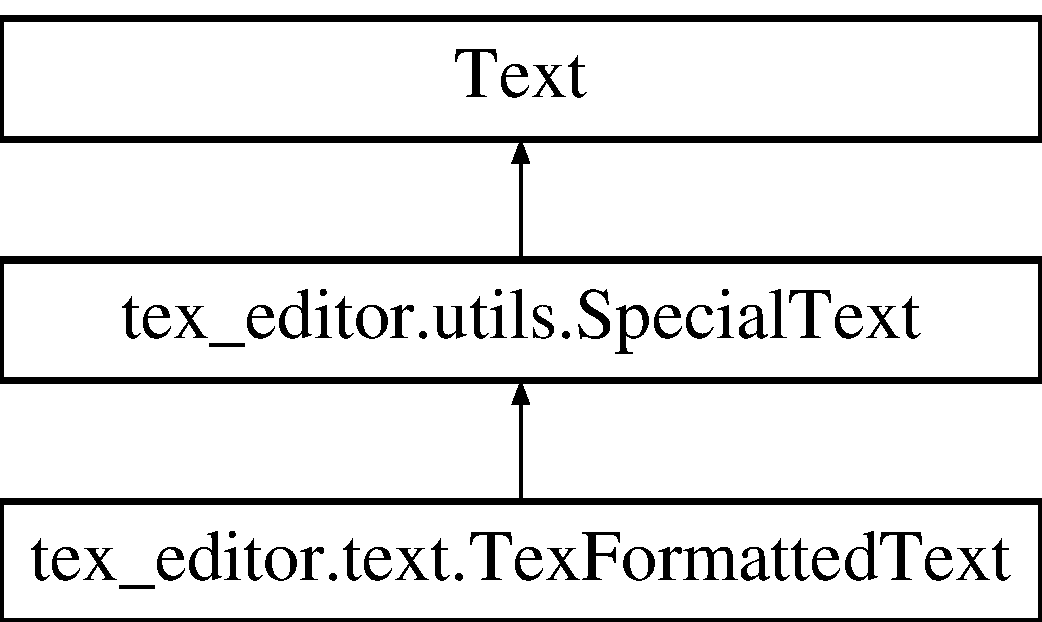
\includegraphics[height=3.000000cm]{classtex__editor_1_1utils_1_1_special_text}
\end{center}
\end{figure}
\subsection*{Fonctions membres publiques}
\begin{DoxyCompactItemize}
\item 
def \hyperlink{classtex__editor_1_1utils_1_1_special_text_ab5ce5add457b9d87567d9e406e0e0d7f}{\+\_\+\+\_\+init\+\_\+\+\_\+} (self, master=None, args, kwargs)
\item 
def \hyperlink{classtex__editor_1_1utils_1_1_special_text_ac86588cdecd42ba520da540c3b53054c}{show\+\_\+tooltip\+\_\+at\+\_\+clicked\+\_\+position} (self, event, \hyperlink{namespacetex__editor_1_1utils_ae4fa308d3c65a5223578baf4c1ec4ddd}{text})
\item 
def \hyperlink{classtex__editor_1_1utils_1_1_special_text_aa2c7f505584004c3a51503b561f88d93}{register\+\_\+structure\+\_\+tag} (self, tag)
\item 
def \hyperlink{classtex__editor_1_1utils_1_1_special_text_ac2a86818f880670a440941efe6aac1c3}{register\+\_\+error\+\_\+tag} (self, tag)
\item 
def \hyperlink{classtex__editor_1_1utils_1_1_special_text_aff461b778803c2006cc119f2b3423e7e}{register\+\_\+additional\+\_\+tag} (self, tag)
\item 
def \hyperlink{classtex__editor_1_1utils_1_1_special_text_ad05500b9af029430216d4d8e3ef8dd0c}{remove\+\_\+error\+\_\+tags} (self, begin, end)
\item 
def \hyperlink{classtex__editor_1_1utils_1_1_special_text_a0f84ca56d6989cc55461d13436dac299}{remove\+\_\+additional\+\_\+tags} (self, begin, end)
\item 
def \hyperlink{classtex__editor_1_1utils_1_1_special_text_a3a9a95544f83c8263b1282d4bdb4d24b}{on\+\_\+change}
\item 
def \hyperlink{classtex__editor_1_1utils_1_1_special_text_a8b33099c6026bdd806c3f899b104a670}{tag\+\_\+add} (self, args, kwargs)
\item 
def \hyperlink{classtex__editor_1_1utils_1_1_special_text_a8989286a4a84c502f21438d58cb3bf84}{tag\+\_\+remove} (self, args, kwargs)
\item 
def \hyperlink{classtex__editor_1_1utils_1_1_special_text_a8fe83b25bc52aa9240d159aed2081043}{on\+\_\+scroll} (self, args, kwargs)
\item 
def \hyperlink{classtex__editor_1_1utils_1_1_special_text_adbc4b27e8f31501bee76441b209612e0}{on\+\_\+select\+\_\+all}
\item 
def \hyperlink{classtex__editor_1_1utils_1_1_special_text_adda1583e7a0fea7dd4f1c5a13ad1cbf3}{\+\_\+\+\_\+str\+\_\+\+\_\+} (self)
\item 
def \hyperlink{classtex__editor_1_1utils_1_1_special_text_a6eeb46052643bc78189fde776c810816}{on\+\_\+key}
\item 
def \hyperlink{classtex__editor_1_1utils_1_1_special_text_a7b1081969baa7ac4a02f5ee923ef7186}{insert\+\_\+text}
\item 
def \hyperlink{classtex__editor_1_1utils_1_1_special_text_afc888f5c0bf9de7be4f144718b3fe8fd}{on\+\_\+copy}
\item 
def \hyperlink{classtex__editor_1_1utils_1_1_special_text_a1403cd4dac3022124fa5fbe2c661eacd}{on\+\_\+cut}
\item 
def \hyperlink{classtex__editor_1_1utils_1_1_special_text_ad6631a1cf04694d144470bbe3e109e98}{on\+\_\+paste}
\item 
def \hyperlink{classtex__editor_1_1utils_1_1_special_text_a6b1b1d52a74cf99fc4d49c1737fec8e0}{on\+\_\+find}
\end{DoxyCompactItemize}
\subsection*{Attributs publics}
\begin{DoxyCompactItemize}
\item 
\hyperlink{classtex__editor_1_1utils_1_1_special_text_a92e99a123af2b93e7b7bb69585240f13}{frame}
\item 
\hyperlink{classtex__editor_1_1utils_1_1_special_text_aa01037a9c0d49d806abbc9822c60cc35}{vbar}
\item 
\hyperlink{classtex__editor_1_1utils_1_1_special_text_ab0eb81132ed588c16c3561a8b726619f}{linenumbers}
\item 
\hyperlink{classtex__editor_1_1utils_1_1_special_text_aa8d9c577e09d0f6ad96671552ce38a64}{structurescroller}
\item 
\hyperlink{classtex__editor_1_1utils_1_1_special_text_a7cbbcc511806669887afff4e53bc7d1a}{errorscroller}
\item 
\hyperlink{classtex__editor_1_1utils_1_1_special_text_a6a3b266f1363705b2b96e2430a60621d}{additional\+\_\+tags}
\end{DoxyCompactItemize}


\subsection{Description détaillée}
\begin{DoxyVerb}@class SpecialText
A subclass of Text, scrollable, with line numbers, that adds commands :
- copy
- cut
- paste
- find
- select all

It fires automatically <<Change>> event when the text is modified in a way
such that line numbers should be updated, and catches it.
\end{DoxyVerb}
 

Définition à la ligne 193 du fichier utils.\+py.



\subsection{Documentation des constructeurs et destructeur}
\hypertarget{classtex__editor_1_1utils_1_1_special_text_ab5ce5add457b9d87567d9e406e0e0d7f}{}\index{tex\+\_\+editor\+::utils\+::\+Special\+Text@{tex\+\_\+editor\+::utils\+::\+Special\+Text}!\+\_\+\+\_\+init\+\_\+\+\_\+@{\+\_\+\+\_\+init\+\_\+\+\_\+}}
\index{\+\_\+\+\_\+init\+\_\+\+\_\+@{\+\_\+\+\_\+init\+\_\+\+\_\+}!tex\+\_\+editor\+::utils\+::\+Special\+Text@{tex\+\_\+editor\+::utils\+::\+Special\+Text}}
\subsubsection[{\+\_\+\+\_\+init\+\_\+\+\_\+}]{\setlength{\rightskip}{0pt plus 5cm}def tex\+\_\+editor.\+utils.\+Special\+Text.\+\_\+\+\_\+init\+\_\+\+\_\+ (
\begin{DoxyParamCaption}
\item[{}]{self, }
\item[{}]{master = {\ttfamily None}, }
\item[{}]{args, }
\item[{}]{kwargs}
\end{DoxyParamCaption}
)}\label{classtex__editor_1_1utils_1_1_special_text_ab5ce5add457b9d87567d9e406e0e0d7f}


Définition à la ligne 207 du fichier utils.\+py.



\subsection{Documentation des fonctions membres}
\hypertarget{classtex__editor_1_1utils_1_1_special_text_adda1583e7a0fea7dd4f1c5a13ad1cbf3}{}\index{tex\+\_\+editor\+::utils\+::\+Special\+Text@{tex\+\_\+editor\+::utils\+::\+Special\+Text}!\+\_\+\+\_\+str\+\_\+\+\_\+@{\+\_\+\+\_\+str\+\_\+\+\_\+}}
\index{\+\_\+\+\_\+str\+\_\+\+\_\+@{\+\_\+\+\_\+str\+\_\+\+\_\+}!tex\+\_\+editor\+::utils\+::\+Special\+Text@{tex\+\_\+editor\+::utils\+::\+Special\+Text}}
\subsubsection[{\+\_\+\+\_\+str\+\_\+\+\_\+}]{\setlength{\rightskip}{0pt plus 5cm}def tex\+\_\+editor.\+utils.\+Special\+Text.\+\_\+\+\_\+str\+\_\+\+\_\+ (
\begin{DoxyParamCaption}
\item[{}]{self}
\end{DoxyParamCaption}
)}\label{classtex__editor_1_1utils_1_1_special_text_adda1583e7a0fea7dd4f1c5a13ad1cbf3}


Définition à la ligne 316 du fichier utils.\+py.

\hypertarget{classtex__editor_1_1utils_1_1_special_text_a7b1081969baa7ac4a02f5ee923ef7186}{}\index{tex\+\_\+editor\+::utils\+::\+Special\+Text@{tex\+\_\+editor\+::utils\+::\+Special\+Text}!insert\+\_\+text@{insert\+\_\+text}}
\index{insert\+\_\+text@{insert\+\_\+text}!tex\+\_\+editor\+::utils\+::\+Special\+Text@{tex\+\_\+editor\+::utils\+::\+Special\+Text}}
\subsubsection[{insert\+\_\+text}]{\setlength{\rightskip}{0pt plus 5cm}def tex\+\_\+editor.\+utils.\+Special\+Text.\+insert\+\_\+text (
\begin{DoxyParamCaption}
\item[{}]{self, }
\item[{}]{t, }
\item[{}]{event = {\ttfamily None}}
\end{DoxyParamCaption}
)}\label{classtex__editor_1_1utils_1_1_special_text_a7b1081969baa7ac4a02f5ee923ef7186}
\begin{DoxyVerb}Insert text at the position INSERT and fire a <<Change>> event.
\end{DoxyVerb}
 

Définition à la ligne 327 du fichier utils.\+py.

\hypertarget{classtex__editor_1_1utils_1_1_special_text_a3a9a95544f83c8263b1282d4bdb4d24b}{}\index{tex\+\_\+editor\+::utils\+::\+Special\+Text@{tex\+\_\+editor\+::utils\+::\+Special\+Text}!on\+\_\+change@{on\+\_\+change}}
\index{on\+\_\+change@{on\+\_\+change}!tex\+\_\+editor\+::utils\+::\+Special\+Text@{tex\+\_\+editor\+::utils\+::\+Special\+Text}}
\subsubsection[{on\+\_\+change}]{\setlength{\rightskip}{0pt plus 5cm}def tex\+\_\+editor.\+utils.\+Special\+Text.\+on\+\_\+change (
\begin{DoxyParamCaption}
\item[{}]{self, }
\item[{}]{event = {\ttfamily None}}
\end{DoxyParamCaption}
)}\label{classtex__editor_1_1utils_1_1_special_text_a3a9a95544f83c8263b1282d4bdb4d24b}


Définition à la ligne 284 du fichier utils.\+py.

\hypertarget{classtex__editor_1_1utils_1_1_special_text_afc888f5c0bf9de7be4f144718b3fe8fd}{}\index{tex\+\_\+editor\+::utils\+::\+Special\+Text@{tex\+\_\+editor\+::utils\+::\+Special\+Text}!on\+\_\+copy@{on\+\_\+copy}}
\index{on\+\_\+copy@{on\+\_\+copy}!tex\+\_\+editor\+::utils\+::\+Special\+Text@{tex\+\_\+editor\+::utils\+::\+Special\+Text}}
\subsubsection[{on\+\_\+copy}]{\setlength{\rightskip}{0pt plus 5cm}def tex\+\_\+editor.\+utils.\+Special\+Text.\+on\+\_\+copy (
\begin{DoxyParamCaption}
\item[{}]{self, }
\item[{}]{event = {\ttfamily None}}
\end{DoxyParamCaption}
)}\label{classtex__editor_1_1utils_1_1_special_text_afc888f5c0bf9de7be4f144718b3fe8fd}
\begin{DoxyVerb}Copy the selection in the clipboard.
\end{DoxyVerb}
 

Définition à la ligne 340 du fichier utils.\+py.

\hypertarget{classtex__editor_1_1utils_1_1_special_text_a1403cd4dac3022124fa5fbe2c661eacd}{}\index{tex\+\_\+editor\+::utils\+::\+Special\+Text@{tex\+\_\+editor\+::utils\+::\+Special\+Text}!on\+\_\+cut@{on\+\_\+cut}}
\index{on\+\_\+cut@{on\+\_\+cut}!tex\+\_\+editor\+::utils\+::\+Special\+Text@{tex\+\_\+editor\+::utils\+::\+Special\+Text}}
\subsubsection[{on\+\_\+cut}]{\setlength{\rightskip}{0pt plus 5cm}def tex\+\_\+editor.\+utils.\+Special\+Text.\+on\+\_\+cut (
\begin{DoxyParamCaption}
\item[{}]{self, }
\item[{}]{event = {\ttfamily None}}
\end{DoxyParamCaption}
)}\label{classtex__editor_1_1utils_1_1_special_text_a1403cd4dac3022124fa5fbe2c661eacd}
\begin{DoxyVerb}Cut the selection in the clipboard.
\end{DoxyVerb}
 

Définition à la ligne 352 du fichier utils.\+py.

\hypertarget{classtex__editor_1_1utils_1_1_special_text_a6b1b1d52a74cf99fc4d49c1737fec8e0}{}\index{tex\+\_\+editor\+::utils\+::\+Special\+Text@{tex\+\_\+editor\+::utils\+::\+Special\+Text}!on\+\_\+find@{on\+\_\+find}}
\index{on\+\_\+find@{on\+\_\+find}!tex\+\_\+editor\+::utils\+::\+Special\+Text@{tex\+\_\+editor\+::utils\+::\+Special\+Text}}
\subsubsection[{on\+\_\+find}]{\setlength{\rightskip}{0pt plus 5cm}def tex\+\_\+editor.\+utils.\+Special\+Text.\+on\+\_\+find (
\begin{DoxyParamCaption}
\item[{}]{self, }
\item[{}]{event = {\ttfamily None}}
\end{DoxyParamCaption}
)}\label{classtex__editor_1_1utils_1_1_special_text_a6b1b1d52a74cf99fc4d49c1737fec8e0}
\begin{DoxyVerb}The method has two behaviors :
- if some text is selected, search and find in this part only
- if no text is selected, search in the whole text
\end{DoxyVerb}
 

Définition à la ligne 378 du fichier utils.\+py.

\hypertarget{classtex__editor_1_1utils_1_1_special_text_a6eeb46052643bc78189fde776c810816}{}\index{tex\+\_\+editor\+::utils\+::\+Special\+Text@{tex\+\_\+editor\+::utils\+::\+Special\+Text}!on\+\_\+key@{on\+\_\+key}}
\index{on\+\_\+key@{on\+\_\+key}!tex\+\_\+editor\+::utils\+::\+Special\+Text@{tex\+\_\+editor\+::utils\+::\+Special\+Text}}
\subsubsection[{on\+\_\+key}]{\setlength{\rightskip}{0pt plus 5cm}def tex\+\_\+editor.\+utils.\+Special\+Text.\+on\+\_\+key (
\begin{DoxyParamCaption}
\item[{}]{self, }
\item[{}]{event = {\ttfamily None}}
\end{DoxyParamCaption}
)}\label{classtex__editor_1_1utils_1_1_special_text_a6eeb46052643bc78189fde776c810816}
\begin{DoxyVerb}Generate a <<Change>> event when any key is pressed, to redraw line
numbers and scroll panel.
\end{DoxyVerb}
 

Définition à la ligne 319 du fichier utils.\+py.

\hypertarget{classtex__editor_1_1utils_1_1_special_text_ad6631a1cf04694d144470bbe3e109e98}{}\index{tex\+\_\+editor\+::utils\+::\+Special\+Text@{tex\+\_\+editor\+::utils\+::\+Special\+Text}!on\+\_\+paste@{on\+\_\+paste}}
\index{on\+\_\+paste@{on\+\_\+paste}!tex\+\_\+editor\+::utils\+::\+Special\+Text@{tex\+\_\+editor\+::utils\+::\+Special\+Text}}
\subsubsection[{on\+\_\+paste}]{\setlength{\rightskip}{0pt plus 5cm}def tex\+\_\+editor.\+utils.\+Special\+Text.\+on\+\_\+paste (
\begin{DoxyParamCaption}
\item[{}]{self, }
\item[{}]{event = {\ttfamily None}}
\end{DoxyParamCaption}
)}\label{classtex__editor_1_1utils_1_1_special_text_ad6631a1cf04694d144470bbe3e109e98}
\begin{DoxyVerb}Paste the clipboard's contents.
\end{DoxyVerb}
 

Définition à la ligne 365 du fichier utils.\+py.

\hypertarget{classtex__editor_1_1utils_1_1_special_text_a8fe83b25bc52aa9240d159aed2081043}{}\index{tex\+\_\+editor\+::utils\+::\+Special\+Text@{tex\+\_\+editor\+::utils\+::\+Special\+Text}!on\+\_\+scroll@{on\+\_\+scroll}}
\index{on\+\_\+scroll@{on\+\_\+scroll}!tex\+\_\+editor\+::utils\+::\+Special\+Text@{tex\+\_\+editor\+::utils\+::\+Special\+Text}}
\subsubsection[{on\+\_\+scroll}]{\setlength{\rightskip}{0pt plus 5cm}def tex\+\_\+editor.\+utils.\+Special\+Text.\+on\+\_\+scroll (
\begin{DoxyParamCaption}
\item[{}]{self, }
\item[{}]{args, }
\item[{}]{kwargs}
\end{DoxyParamCaption}
)}\label{classtex__editor_1_1utils_1_1_special_text_a8fe83b25bc52aa9240d159aed2081043}
\begin{DoxyVerb}Generate a <<Change>> event when the text zone is scrolled. This helps
redrawing the line numbers.
\end{DoxyVerb}
 

Définition à la ligne 297 du fichier utils.\+py.

\hypertarget{classtex__editor_1_1utils_1_1_special_text_adbc4b27e8f31501bee76441b209612e0}{}\index{tex\+\_\+editor\+::utils\+::\+Special\+Text@{tex\+\_\+editor\+::utils\+::\+Special\+Text}!on\+\_\+select\+\_\+all@{on\+\_\+select\+\_\+all}}
\index{on\+\_\+select\+\_\+all@{on\+\_\+select\+\_\+all}!tex\+\_\+editor\+::utils\+::\+Special\+Text@{tex\+\_\+editor\+::utils\+::\+Special\+Text}}
\subsubsection[{on\+\_\+select\+\_\+all}]{\setlength{\rightskip}{0pt plus 5cm}def tex\+\_\+editor.\+utils.\+Special\+Text.\+on\+\_\+select\+\_\+all (
\begin{DoxyParamCaption}
\item[{}]{self, }
\item[{}]{event = {\ttfamily None}}
\end{DoxyParamCaption}
)}\label{classtex__editor_1_1utils_1_1_special_text_adbc4b27e8f31501bee76441b209612e0}
\begin{DoxyVerb}Select the whole content of the text zone.
\end{DoxyVerb}
 

Définition à la ligne 306 du fichier utils.\+py.

\hypertarget{classtex__editor_1_1utils_1_1_special_text_aff461b778803c2006cc119f2b3423e7e}{}\index{tex\+\_\+editor\+::utils\+::\+Special\+Text@{tex\+\_\+editor\+::utils\+::\+Special\+Text}!register\+\_\+additional\+\_\+tag@{register\+\_\+additional\+\_\+tag}}
\index{register\+\_\+additional\+\_\+tag@{register\+\_\+additional\+\_\+tag}!tex\+\_\+editor\+::utils\+::\+Special\+Text@{tex\+\_\+editor\+::utils\+::\+Special\+Text}}
\subsubsection[{register\+\_\+additional\+\_\+tag}]{\setlength{\rightskip}{0pt plus 5cm}def tex\+\_\+editor.\+utils.\+Special\+Text.\+register\+\_\+additional\+\_\+tag (
\begin{DoxyParamCaption}
\item[{}]{self, }
\item[{}]{tag}
\end{DoxyParamCaption}
)}\label{classtex__editor_1_1utils_1_1_special_text_aff461b778803c2006cc119f2b3423e7e}


Définition à la ligne 273 du fichier utils.\+py.

\hypertarget{classtex__editor_1_1utils_1_1_special_text_ac2a86818f880670a440941efe6aac1c3}{}\index{tex\+\_\+editor\+::utils\+::\+Special\+Text@{tex\+\_\+editor\+::utils\+::\+Special\+Text}!register\+\_\+error\+\_\+tag@{register\+\_\+error\+\_\+tag}}
\index{register\+\_\+error\+\_\+tag@{register\+\_\+error\+\_\+tag}!tex\+\_\+editor\+::utils\+::\+Special\+Text@{tex\+\_\+editor\+::utils\+::\+Special\+Text}}
\subsubsection[{register\+\_\+error\+\_\+tag}]{\setlength{\rightskip}{0pt plus 5cm}def tex\+\_\+editor.\+utils.\+Special\+Text.\+register\+\_\+error\+\_\+tag (
\begin{DoxyParamCaption}
\item[{}]{self, }
\item[{}]{tag}
\end{DoxyParamCaption}
)}\label{classtex__editor_1_1utils_1_1_special_text_ac2a86818f880670a440941efe6aac1c3}


Définition à la ligne 270 du fichier utils.\+py.

\hypertarget{classtex__editor_1_1utils_1_1_special_text_aa2c7f505584004c3a51503b561f88d93}{}\index{tex\+\_\+editor\+::utils\+::\+Special\+Text@{tex\+\_\+editor\+::utils\+::\+Special\+Text}!register\+\_\+structure\+\_\+tag@{register\+\_\+structure\+\_\+tag}}
\index{register\+\_\+structure\+\_\+tag@{register\+\_\+structure\+\_\+tag}!tex\+\_\+editor\+::utils\+::\+Special\+Text@{tex\+\_\+editor\+::utils\+::\+Special\+Text}}
\subsubsection[{register\+\_\+structure\+\_\+tag}]{\setlength{\rightskip}{0pt plus 5cm}def tex\+\_\+editor.\+utils.\+Special\+Text.\+register\+\_\+structure\+\_\+tag (
\begin{DoxyParamCaption}
\item[{}]{self, }
\item[{}]{tag}
\end{DoxyParamCaption}
)}\label{classtex__editor_1_1utils_1_1_special_text_aa2c7f505584004c3a51503b561f88d93}


Définition à la ligne 267 du fichier utils.\+py.

\hypertarget{classtex__editor_1_1utils_1_1_special_text_a0f84ca56d6989cc55461d13436dac299}{}\index{tex\+\_\+editor\+::utils\+::\+Special\+Text@{tex\+\_\+editor\+::utils\+::\+Special\+Text}!remove\+\_\+additional\+\_\+tags@{remove\+\_\+additional\+\_\+tags}}
\index{remove\+\_\+additional\+\_\+tags@{remove\+\_\+additional\+\_\+tags}!tex\+\_\+editor\+::utils\+::\+Special\+Text@{tex\+\_\+editor\+::utils\+::\+Special\+Text}}
\subsubsection[{remove\+\_\+additional\+\_\+tags}]{\setlength{\rightskip}{0pt plus 5cm}def tex\+\_\+editor.\+utils.\+Special\+Text.\+remove\+\_\+additional\+\_\+tags (
\begin{DoxyParamCaption}
\item[{}]{self, }
\item[{}]{begin, }
\item[{}]{end}
\end{DoxyParamCaption}
)}\label{classtex__editor_1_1utils_1_1_special_text_a0f84ca56d6989cc55461d13436dac299}


Définition à la ligne 280 du fichier utils.\+py.

\hypertarget{classtex__editor_1_1utils_1_1_special_text_ad05500b9af029430216d4d8e3ef8dd0c}{}\index{tex\+\_\+editor\+::utils\+::\+Special\+Text@{tex\+\_\+editor\+::utils\+::\+Special\+Text}!remove\+\_\+error\+\_\+tags@{remove\+\_\+error\+\_\+tags}}
\index{remove\+\_\+error\+\_\+tags@{remove\+\_\+error\+\_\+tags}!tex\+\_\+editor\+::utils\+::\+Special\+Text@{tex\+\_\+editor\+::utils\+::\+Special\+Text}}
\subsubsection[{remove\+\_\+error\+\_\+tags}]{\setlength{\rightskip}{0pt plus 5cm}def tex\+\_\+editor.\+utils.\+Special\+Text.\+remove\+\_\+error\+\_\+tags (
\begin{DoxyParamCaption}
\item[{}]{self, }
\item[{}]{begin, }
\item[{}]{end}
\end{DoxyParamCaption}
)}\label{classtex__editor_1_1utils_1_1_special_text_ad05500b9af029430216d4d8e3ef8dd0c}


Définition à la ligne 276 du fichier utils.\+py.

\hypertarget{classtex__editor_1_1utils_1_1_special_text_ac86588cdecd42ba520da540c3b53054c}{}\index{tex\+\_\+editor\+::utils\+::\+Special\+Text@{tex\+\_\+editor\+::utils\+::\+Special\+Text}!show\+\_\+tooltip\+\_\+at\+\_\+clicked\+\_\+position@{show\+\_\+tooltip\+\_\+at\+\_\+clicked\+\_\+position}}
\index{show\+\_\+tooltip\+\_\+at\+\_\+clicked\+\_\+position@{show\+\_\+tooltip\+\_\+at\+\_\+clicked\+\_\+position}!tex\+\_\+editor\+::utils\+::\+Special\+Text@{tex\+\_\+editor\+::utils\+::\+Special\+Text}}
\subsubsection[{show\+\_\+tooltip\+\_\+at\+\_\+clicked\+\_\+position}]{\setlength{\rightskip}{0pt plus 5cm}def tex\+\_\+editor.\+utils.\+Special\+Text.\+show\+\_\+tooltip\+\_\+at\+\_\+clicked\+\_\+position (
\begin{DoxyParamCaption}
\item[{}]{self, }
\item[{}]{event, }
\item[{}]{text}
\end{DoxyParamCaption}
)}\label{classtex__editor_1_1utils_1_1_special_text_ac86588cdecd42ba520da540c3b53054c}
\begin{DoxyVerb}Show a tooltip with the text given in argument, at the position
that was clicked in the text zone.
\end{DoxyVerb}
 

Définition à la ligne 260 du fichier utils.\+py.

\hypertarget{classtex__editor_1_1utils_1_1_special_text_a8b33099c6026bdd806c3f899b104a670}{}\index{tex\+\_\+editor\+::utils\+::\+Special\+Text@{tex\+\_\+editor\+::utils\+::\+Special\+Text}!tag\+\_\+add@{tag\+\_\+add}}
\index{tag\+\_\+add@{tag\+\_\+add}!tex\+\_\+editor\+::utils\+::\+Special\+Text@{tex\+\_\+editor\+::utils\+::\+Special\+Text}}
\subsubsection[{tag\+\_\+add}]{\setlength{\rightskip}{0pt plus 5cm}def tex\+\_\+editor.\+utils.\+Special\+Text.\+tag\+\_\+add (
\begin{DoxyParamCaption}
\item[{}]{self, }
\item[{}]{args, }
\item[{}]{kwargs}
\end{DoxyParamCaption}
)}\label{classtex__editor_1_1utils_1_1_special_text_a8b33099c6026bdd806c3f899b104a670}


Définition à la ligne 289 du fichier utils.\+py.

\hypertarget{classtex__editor_1_1utils_1_1_special_text_a8989286a4a84c502f21438d58cb3bf84}{}\index{tex\+\_\+editor\+::utils\+::\+Special\+Text@{tex\+\_\+editor\+::utils\+::\+Special\+Text}!tag\+\_\+remove@{tag\+\_\+remove}}
\index{tag\+\_\+remove@{tag\+\_\+remove}!tex\+\_\+editor\+::utils\+::\+Special\+Text@{tex\+\_\+editor\+::utils\+::\+Special\+Text}}
\subsubsection[{tag\+\_\+remove}]{\setlength{\rightskip}{0pt plus 5cm}def tex\+\_\+editor.\+utils.\+Special\+Text.\+tag\+\_\+remove (
\begin{DoxyParamCaption}
\item[{}]{self, }
\item[{}]{args, }
\item[{}]{kwargs}
\end{DoxyParamCaption}
)}\label{classtex__editor_1_1utils_1_1_special_text_a8989286a4a84c502f21438d58cb3bf84}


Définition à la ligne 293 du fichier utils.\+py.



\subsection{Documentation des données membres}
\hypertarget{classtex__editor_1_1utils_1_1_special_text_a6a3b266f1363705b2b96e2430a60621d}{}\index{tex\+\_\+editor\+::utils\+::\+Special\+Text@{tex\+\_\+editor\+::utils\+::\+Special\+Text}!additional\+\_\+tags@{additional\+\_\+tags}}
\index{additional\+\_\+tags@{additional\+\_\+tags}!tex\+\_\+editor\+::utils\+::\+Special\+Text@{tex\+\_\+editor\+::utils\+::\+Special\+Text}}
\subsubsection[{additional\+\_\+tags}]{\setlength{\rightskip}{0pt plus 5cm}tex\+\_\+editor.\+utils.\+Special\+Text.\+additional\+\_\+tags}\label{classtex__editor_1_1utils_1_1_special_text_a6a3b266f1363705b2b96e2430a60621d}


Définition à la ligne 258 du fichier utils.\+py.

\hypertarget{classtex__editor_1_1utils_1_1_special_text_a7cbbcc511806669887afff4e53bc7d1a}{}\index{tex\+\_\+editor\+::utils\+::\+Special\+Text@{tex\+\_\+editor\+::utils\+::\+Special\+Text}!errorscroller@{errorscroller}}
\index{errorscroller@{errorscroller}!tex\+\_\+editor\+::utils\+::\+Special\+Text@{tex\+\_\+editor\+::utils\+::\+Special\+Text}}
\subsubsection[{errorscroller}]{\setlength{\rightskip}{0pt plus 5cm}tex\+\_\+editor.\+utils.\+Special\+Text.\+errorscroller}\label{classtex__editor_1_1utils_1_1_special_text_a7cbbcc511806669887afff4e53bc7d1a}


Définition à la ligne 227 du fichier utils.\+py.

\hypertarget{classtex__editor_1_1utils_1_1_special_text_a92e99a123af2b93e7b7bb69585240f13}{}\index{tex\+\_\+editor\+::utils\+::\+Special\+Text@{tex\+\_\+editor\+::utils\+::\+Special\+Text}!frame@{frame}}
\index{frame@{frame}!tex\+\_\+editor\+::utils\+::\+Special\+Text@{tex\+\_\+editor\+::utils\+::\+Special\+Text}}
\subsubsection[{frame}]{\setlength{\rightskip}{0pt plus 5cm}tex\+\_\+editor.\+utils.\+Special\+Text.\+frame}\label{classtex__editor_1_1utils_1_1_special_text_a92e99a123af2b93e7b7bb69585240f13}


Définition à la ligne 208 du fichier utils.\+py.

\hypertarget{classtex__editor_1_1utils_1_1_special_text_ab0eb81132ed588c16c3561a8b726619f}{}\index{tex\+\_\+editor\+::utils\+::\+Special\+Text@{tex\+\_\+editor\+::utils\+::\+Special\+Text}!linenumbers@{linenumbers}}
\index{linenumbers@{linenumbers}!tex\+\_\+editor\+::utils\+::\+Special\+Text@{tex\+\_\+editor\+::utils\+::\+Special\+Text}}
\subsubsection[{linenumbers}]{\setlength{\rightskip}{0pt plus 5cm}tex\+\_\+editor.\+utils.\+Special\+Text.\+linenumbers}\label{classtex__editor_1_1utils_1_1_special_text_ab0eb81132ed588c16c3561a8b726619f}


Définition à la ligne 219 du fichier utils.\+py.

\hypertarget{classtex__editor_1_1utils_1_1_special_text_aa8d9c577e09d0f6ad96671552ce38a64}{}\index{tex\+\_\+editor\+::utils\+::\+Special\+Text@{tex\+\_\+editor\+::utils\+::\+Special\+Text}!structurescroller@{structurescroller}}
\index{structurescroller@{structurescroller}!tex\+\_\+editor\+::utils\+::\+Special\+Text@{tex\+\_\+editor\+::utils\+::\+Special\+Text}}
\subsubsection[{structurescroller}]{\setlength{\rightskip}{0pt plus 5cm}tex\+\_\+editor.\+utils.\+Special\+Text.\+structurescroller}\label{classtex__editor_1_1utils_1_1_special_text_aa8d9c577e09d0f6ad96671552ce38a64}


Définition à la ligne 223 du fichier utils.\+py.

\hypertarget{classtex__editor_1_1utils_1_1_special_text_aa01037a9c0d49d806abbc9822c60cc35}{}\index{tex\+\_\+editor\+::utils\+::\+Special\+Text@{tex\+\_\+editor\+::utils\+::\+Special\+Text}!vbar@{vbar}}
\index{vbar@{vbar}!tex\+\_\+editor\+::utils\+::\+Special\+Text@{tex\+\_\+editor\+::utils\+::\+Special\+Text}}
\subsubsection[{vbar}]{\setlength{\rightskip}{0pt plus 5cm}tex\+\_\+editor.\+utils.\+Special\+Text.\+vbar}\label{classtex__editor_1_1utils_1_1_special_text_aa01037a9c0d49d806abbc9822c60cc35}


Définition à la ligne 209 du fichier utils.\+py.



La documentation de cette classe a été générée à partir du fichier suivant \+:\begin{DoxyCompactItemize}
\item 
src/tex\+\_\+editor/\hyperlink{utils_8py}{utils.\+py}\end{DoxyCompactItemize}

\hypertarget{classtex__editor_1_1utils_1_1_tags_scroller}{}\section{Référence de la classe tex\+\_\+editor.\+utils.\+Tags\+Scroller}
\label{classtex__editor_1_1utils_1_1_tags_scroller}\index{tex\+\_\+editor.\+utils.\+Tags\+Scroller@{tex\+\_\+editor.\+utils.\+Tags\+Scroller}}
Graphe d\textquotesingle{}héritage de tex\+\_\+editor.\+utils.\+Tags\+Scroller\+:\begin{figure}[H]
\begin{center}
\leavevmode
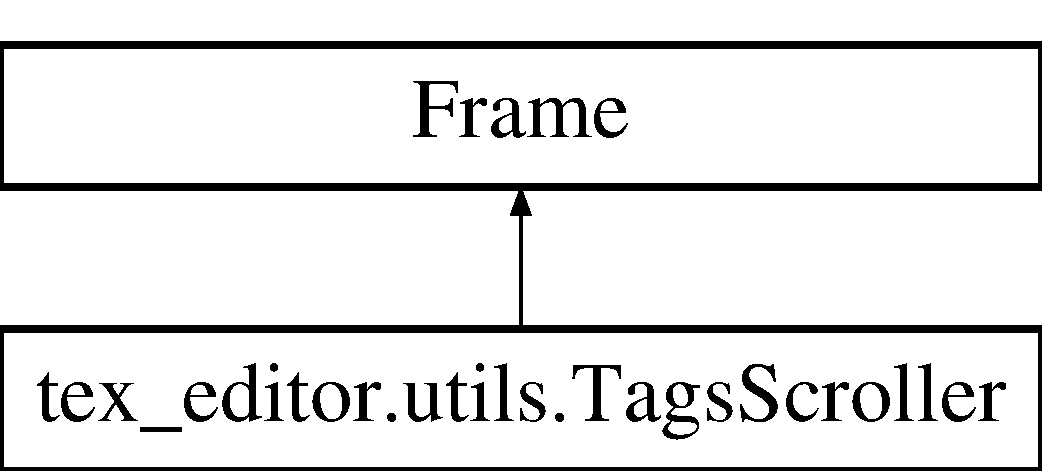
\includegraphics[height=2.000000cm]{classtex__editor_1_1utils_1_1_tags_scroller}
\end{center}
\end{figure}
\subsection*{Fonctions membres publiques}
\begin{DoxyCompactItemize}
\item 
def \hyperlink{classtex__editor_1_1utils_1_1_tags_scroller_a04847d8e03096beb46a820052bb165b1}{\+\_\+\+\_\+init\+\_\+\+\_\+} (self, args, kwargs)
\item 
def \hyperlink{classtex__editor_1_1utils_1_1_tags_scroller_ac2c15ab31c416af4976efc24bb2408bd}{on\+\_\+down} (self, event)
\item 
def \hyperlink{classtex__editor_1_1utils_1_1_tags_scroller_a238fd796f7ac965d377b74ecf057d1af}{on\+\_\+up} (self, event)
\item 
def \hyperlink{classtex__editor_1_1utils_1_1_tags_scroller_ad7cd936a75219c4e33cbb39219e41c35}{attach} (self, \hyperlink{classtex__editor_1_1utils_1_1_tags_scroller_a19ed18ecd55f3bfe63a8d5e4717d0067}{textw})
\item 
def \hyperlink{classtex__editor_1_1utils_1_1_tags_scroller_a8e022b12638ba173b6801136e318759d}{register\+\_\+tag} (self, t)
\item 
def \hyperlink{classtex__editor_1_1utils_1_1_tags_scroller_acf7fab0a469d21f79befddb50aa65559}{on\+\_\+mouse\+\_\+select}
\item 
def \hyperlink{classtex__editor_1_1utils_1_1_tags_scroller_afbae051467ce0f0b73bce32f5d80c2e9}{on\+\_\+select}
\item 
def \hyperlink{classtex__editor_1_1utils_1_1_tags_scroller_a84633bb40ca72ed20d83b096e9cecfe5}{redraw} (self, args)
\end{DoxyCompactItemize}
\subsection*{Attributs publics}
\begin{DoxyCompactItemize}
\item 
\hyperlink{classtex__editor_1_1utils_1_1_tags_scroller_a2949d287fca8a09b2a0b56bcf2992e34}{scrollbar}
\item 
\hyperlink{classtex__editor_1_1utils_1_1_tags_scroller_a19ed18ecd55f3bfe63a8d5e4717d0067}{textw}
\item 
\hyperlink{classtex__editor_1_1utils_1_1_tags_scroller_a739235d43d2905d695fd3233b44cd898}{lbox}
\item 
\hyperlink{classtex__editor_1_1utils_1_1_tags_scroller_a6de5e12e332d5ffe891ecb87e3c8caa6}{registered}
\item 
\hyperlink{classtex__editor_1_1utils_1_1_tags_scroller_a5304ca2579118d4cb5f8575a9e836907}{selection}
\end{DoxyCompactItemize}


\subsection{Description détaillée}


Définition à la ligne 71 du fichier utils.\+py.



\subsection{Documentation des constructeurs et destructeur}
\hypertarget{classtex__editor_1_1utils_1_1_tags_scroller_a04847d8e03096beb46a820052bb165b1}{}\index{tex\+\_\+editor\+::utils\+::\+Tags\+Scroller@{tex\+\_\+editor\+::utils\+::\+Tags\+Scroller}!\+\_\+\+\_\+init\+\_\+\+\_\+@{\+\_\+\+\_\+init\+\_\+\+\_\+}}
\index{\+\_\+\+\_\+init\+\_\+\+\_\+@{\+\_\+\+\_\+init\+\_\+\+\_\+}!tex\+\_\+editor\+::utils\+::\+Tags\+Scroller@{tex\+\_\+editor\+::utils\+::\+Tags\+Scroller}}
\subsubsection[{\+\_\+\+\_\+init\+\_\+\+\_\+}]{\setlength{\rightskip}{0pt plus 5cm}def tex\+\_\+editor.\+utils.\+Tags\+Scroller.\+\_\+\+\_\+init\+\_\+\+\_\+ (
\begin{DoxyParamCaption}
\item[{}]{self, }
\item[{}]{args, }
\item[{}]{kwargs}
\end{DoxyParamCaption}
)}\label{classtex__editor_1_1utils_1_1_tags_scroller_a04847d8e03096beb46a820052bb165b1}


Définition à la ligne 73 du fichier utils.\+py.



\subsection{Documentation des fonctions membres}
\hypertarget{classtex__editor_1_1utils_1_1_tags_scroller_ad7cd936a75219c4e33cbb39219e41c35}{}\index{tex\+\_\+editor\+::utils\+::\+Tags\+Scroller@{tex\+\_\+editor\+::utils\+::\+Tags\+Scroller}!attach@{attach}}
\index{attach@{attach}!tex\+\_\+editor\+::utils\+::\+Tags\+Scroller@{tex\+\_\+editor\+::utils\+::\+Tags\+Scroller}}
\subsubsection[{attach}]{\setlength{\rightskip}{0pt plus 5cm}def tex\+\_\+editor.\+utils.\+Tags\+Scroller.\+attach (
\begin{DoxyParamCaption}
\item[{}]{self, }
\item[{}]{textw}
\end{DoxyParamCaption}
)}\label{classtex__editor_1_1utils_1_1_tags_scroller_ad7cd936a75219c4e33cbb39219e41c35}


Définition à la ligne 110 du fichier utils.\+py.

\hypertarget{classtex__editor_1_1utils_1_1_tags_scroller_ac2c15ab31c416af4976efc24bb2408bd}{}\index{tex\+\_\+editor\+::utils\+::\+Tags\+Scroller@{tex\+\_\+editor\+::utils\+::\+Tags\+Scroller}!on\+\_\+down@{on\+\_\+down}}
\index{on\+\_\+down@{on\+\_\+down}!tex\+\_\+editor\+::utils\+::\+Tags\+Scroller@{tex\+\_\+editor\+::utils\+::\+Tags\+Scroller}}
\subsubsection[{on\+\_\+down}]{\setlength{\rightskip}{0pt plus 5cm}def tex\+\_\+editor.\+utils.\+Tags\+Scroller.\+on\+\_\+down (
\begin{DoxyParamCaption}
\item[{}]{self, }
\item[{}]{event}
\end{DoxyParamCaption}
)}\label{classtex__editor_1_1utils_1_1_tags_scroller_ac2c15ab31c416af4976efc24bb2408bd}


Définition à la ligne 96 du fichier utils.\+py.

\hypertarget{classtex__editor_1_1utils_1_1_tags_scroller_acf7fab0a469d21f79befddb50aa65559}{}\index{tex\+\_\+editor\+::utils\+::\+Tags\+Scroller@{tex\+\_\+editor\+::utils\+::\+Tags\+Scroller}!on\+\_\+mouse\+\_\+select@{on\+\_\+mouse\+\_\+select}}
\index{on\+\_\+mouse\+\_\+select@{on\+\_\+mouse\+\_\+select}!tex\+\_\+editor\+::utils\+::\+Tags\+Scroller@{tex\+\_\+editor\+::utils\+::\+Tags\+Scroller}}
\subsubsection[{on\+\_\+mouse\+\_\+select}]{\setlength{\rightskip}{0pt plus 5cm}def tex\+\_\+editor.\+utils.\+Tags\+Scroller.\+on\+\_\+mouse\+\_\+select (
\begin{DoxyParamCaption}
\item[{}]{self, }
\item[{}]{event = {\ttfamily None}}
\end{DoxyParamCaption}
)}\label{classtex__editor_1_1utils_1_1_tags_scroller_acf7fab0a469d21f79befddb50aa65559}


Définition à la ligne 116 du fichier utils.\+py.

\hypertarget{classtex__editor_1_1utils_1_1_tags_scroller_afbae051467ce0f0b73bce32f5d80c2e9}{}\index{tex\+\_\+editor\+::utils\+::\+Tags\+Scroller@{tex\+\_\+editor\+::utils\+::\+Tags\+Scroller}!on\+\_\+select@{on\+\_\+select}}
\index{on\+\_\+select@{on\+\_\+select}!tex\+\_\+editor\+::utils\+::\+Tags\+Scroller@{tex\+\_\+editor\+::utils\+::\+Tags\+Scroller}}
\subsubsection[{on\+\_\+select}]{\setlength{\rightskip}{0pt plus 5cm}def tex\+\_\+editor.\+utils.\+Tags\+Scroller.\+on\+\_\+select (
\begin{DoxyParamCaption}
\item[{}]{self, }
\item[{}]{event = {\ttfamily None}}
\end{DoxyParamCaption}
)}\label{classtex__editor_1_1utils_1_1_tags_scroller_afbae051467ce0f0b73bce32f5d80c2e9}


Définition à la ligne 122 du fichier utils.\+py.

\hypertarget{classtex__editor_1_1utils_1_1_tags_scroller_a238fd796f7ac965d377b74ecf057d1af}{}\index{tex\+\_\+editor\+::utils\+::\+Tags\+Scroller@{tex\+\_\+editor\+::utils\+::\+Tags\+Scroller}!on\+\_\+up@{on\+\_\+up}}
\index{on\+\_\+up@{on\+\_\+up}!tex\+\_\+editor\+::utils\+::\+Tags\+Scroller@{tex\+\_\+editor\+::utils\+::\+Tags\+Scroller}}
\subsubsection[{on\+\_\+up}]{\setlength{\rightskip}{0pt plus 5cm}def tex\+\_\+editor.\+utils.\+Tags\+Scroller.\+on\+\_\+up (
\begin{DoxyParamCaption}
\item[{}]{self, }
\item[{}]{event}
\end{DoxyParamCaption}
)}\label{classtex__editor_1_1utils_1_1_tags_scroller_a238fd796f7ac965d377b74ecf057d1af}


Définition à la ligne 103 du fichier utils.\+py.

\hypertarget{classtex__editor_1_1utils_1_1_tags_scroller_a84633bb40ca72ed20d83b096e9cecfe5}{}\index{tex\+\_\+editor\+::utils\+::\+Tags\+Scroller@{tex\+\_\+editor\+::utils\+::\+Tags\+Scroller}!redraw@{redraw}}
\index{redraw@{redraw}!tex\+\_\+editor\+::utils\+::\+Tags\+Scroller@{tex\+\_\+editor\+::utils\+::\+Tags\+Scroller}}
\subsubsection[{redraw}]{\setlength{\rightskip}{0pt plus 5cm}def tex\+\_\+editor.\+utils.\+Tags\+Scroller.\+redraw (
\begin{DoxyParamCaption}
\item[{}]{self, }
\item[{}]{args}
\end{DoxyParamCaption}
)}\label{classtex__editor_1_1utils_1_1_tags_scroller_a84633bb40ca72ed20d83b096e9cecfe5}


Définition à la ligne 131 du fichier utils.\+py.

\hypertarget{classtex__editor_1_1utils_1_1_tags_scroller_a8e022b12638ba173b6801136e318759d}{}\index{tex\+\_\+editor\+::utils\+::\+Tags\+Scroller@{tex\+\_\+editor\+::utils\+::\+Tags\+Scroller}!register\+\_\+tag@{register\+\_\+tag}}
\index{register\+\_\+tag@{register\+\_\+tag}!tex\+\_\+editor\+::utils\+::\+Tags\+Scroller@{tex\+\_\+editor\+::utils\+::\+Tags\+Scroller}}
\subsubsection[{register\+\_\+tag}]{\setlength{\rightskip}{0pt plus 5cm}def tex\+\_\+editor.\+utils.\+Tags\+Scroller.\+register\+\_\+tag (
\begin{DoxyParamCaption}
\item[{}]{self, }
\item[{}]{t}
\end{DoxyParamCaption}
)}\label{classtex__editor_1_1utils_1_1_tags_scroller_a8e022b12638ba173b6801136e318759d}


Définition à la ligne 113 du fichier utils.\+py.



\subsection{Documentation des données membres}
\hypertarget{classtex__editor_1_1utils_1_1_tags_scroller_a739235d43d2905d695fd3233b44cd898}{}\index{tex\+\_\+editor\+::utils\+::\+Tags\+Scroller@{tex\+\_\+editor\+::utils\+::\+Tags\+Scroller}!lbox@{lbox}}
\index{lbox@{lbox}!tex\+\_\+editor\+::utils\+::\+Tags\+Scroller@{tex\+\_\+editor\+::utils\+::\+Tags\+Scroller}}
\subsubsection[{lbox}]{\setlength{\rightskip}{0pt plus 5cm}tex\+\_\+editor.\+utils.\+Tags\+Scroller.\+lbox}\label{classtex__editor_1_1utils_1_1_tags_scroller_a739235d43d2905d695fd3233b44cd898}


Définition à la ligne 80 du fichier utils.\+py.

\hypertarget{classtex__editor_1_1utils_1_1_tags_scroller_a6de5e12e332d5ffe891ecb87e3c8caa6}{}\index{tex\+\_\+editor\+::utils\+::\+Tags\+Scroller@{tex\+\_\+editor\+::utils\+::\+Tags\+Scroller}!registered@{registered}}
\index{registered@{registered}!tex\+\_\+editor\+::utils\+::\+Tags\+Scroller@{tex\+\_\+editor\+::utils\+::\+Tags\+Scroller}}
\subsubsection[{registered}]{\setlength{\rightskip}{0pt plus 5cm}tex\+\_\+editor.\+utils.\+Tags\+Scroller.\+registered}\label{classtex__editor_1_1utils_1_1_tags_scroller_a6de5e12e332d5ffe891ecb87e3c8caa6}


Définition à la ligne 88 du fichier utils.\+py.

\hypertarget{classtex__editor_1_1utils_1_1_tags_scroller_a2949d287fca8a09b2a0b56bcf2992e34}{}\index{tex\+\_\+editor\+::utils\+::\+Tags\+Scroller@{tex\+\_\+editor\+::utils\+::\+Tags\+Scroller}!scrollbar@{scrollbar}}
\index{scrollbar@{scrollbar}!tex\+\_\+editor\+::utils\+::\+Tags\+Scroller@{tex\+\_\+editor\+::utils\+::\+Tags\+Scroller}}
\subsubsection[{scrollbar}]{\setlength{\rightskip}{0pt plus 5cm}tex\+\_\+editor.\+utils.\+Tags\+Scroller.\+scrollbar}\label{classtex__editor_1_1utils_1_1_tags_scroller_a2949d287fca8a09b2a0b56bcf2992e34}


Définition à la ligne 77 du fichier utils.\+py.

\hypertarget{classtex__editor_1_1utils_1_1_tags_scroller_a5304ca2579118d4cb5f8575a9e836907}{}\index{tex\+\_\+editor\+::utils\+::\+Tags\+Scroller@{tex\+\_\+editor\+::utils\+::\+Tags\+Scroller}!selection@{selection}}
\index{selection@{selection}!tex\+\_\+editor\+::utils\+::\+Tags\+Scroller@{tex\+\_\+editor\+::utils\+::\+Tags\+Scroller}}
\subsubsection[{selection}]{\setlength{\rightskip}{0pt plus 5cm}tex\+\_\+editor.\+utils.\+Tags\+Scroller.\+selection}\label{classtex__editor_1_1utils_1_1_tags_scroller_a5304ca2579118d4cb5f8575a9e836907}


Définition à la ligne 89 du fichier utils.\+py.

\hypertarget{classtex__editor_1_1utils_1_1_tags_scroller_a19ed18ecd55f3bfe63a8d5e4717d0067}{}\index{tex\+\_\+editor\+::utils\+::\+Tags\+Scroller@{tex\+\_\+editor\+::utils\+::\+Tags\+Scroller}!textw@{textw}}
\index{textw@{textw}!tex\+\_\+editor\+::utils\+::\+Tags\+Scroller@{tex\+\_\+editor\+::utils\+::\+Tags\+Scroller}}
\subsubsection[{textw}]{\setlength{\rightskip}{0pt plus 5cm}tex\+\_\+editor.\+utils.\+Tags\+Scroller.\+textw}\label{classtex__editor_1_1utils_1_1_tags_scroller_a19ed18ecd55f3bfe63a8d5e4717d0067}


Définition à la ligne 79 du fichier utils.\+py.



La documentation de cette classe a été générée à partir du fichier suivant \+:\begin{DoxyCompactItemize}
\item 
src/tex\+\_\+editor/\hyperlink{utils_8py}{utils.\+py}\end{DoxyCompactItemize}

\hypertarget{classtex__editor_1_1text_1_1_tex_formatted_text}{}\section{Référence de la classe tex\+\_\+editor.\+text.\+Tex\+Formatted\+Text}
\label{classtex__editor_1_1text_1_1_tex_formatted_text}\index{tex\+\_\+editor.\+text.\+Tex\+Formatted\+Text@{tex\+\_\+editor.\+text.\+Tex\+Formatted\+Text}}
Graphe d\textquotesingle{}héritage de tex\+\_\+editor.\+text.\+Tex\+Formatted\+Text\+:\begin{figure}[H]
\begin{center}
\leavevmode
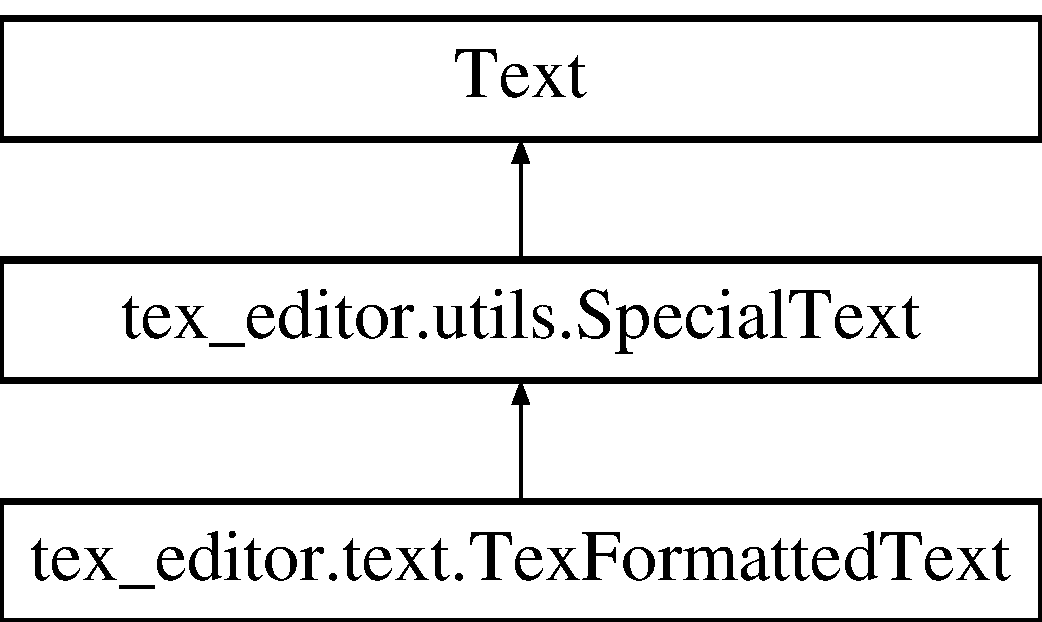
\includegraphics[height=3.000000cm]{classtex__editor_1_1text_1_1_tex_formatted_text}
\end{center}
\end{figure}
\subsection*{Fonctions membres publiques}
\begin{DoxyCompactItemize}
\item 
def \hyperlink{classtex__editor_1_1text_1_1_tex_formatted_text_a95e8a9bcd6a678649ca85e0e30c00086}{\+\_\+\+\_\+init\+\_\+\+\_\+} (self, master=None, args, kwargs)
\item 
def \hyperlink{classtex__editor_1_1text_1_1_tex_formatted_text_adb723d51115ad49dfbde9f4ea42d68c5}{input\+\_\+formatted\+\_\+text} (self, inpt)
\item 
def \hyperlink{classtex__editor_1_1text_1_1_tex_formatted_text_a9893cfadcf978e03331bc3f973364ba4}{input\+\_\+tex\+\_\+with\+\_\+comments} (self, inpt)
\item 
def \hyperlink{classtex__editor_1_1text_1_1_tex_formatted_text_af6ad1e3b0b89c55897e2618f2419aec9}{get\+\_\+tex\+\_\+formatted\+\_\+text}
\item 
def \hyperlink{classtex__editor_1_1text_1_1_tex_formatted_text_a68bbdd9ab36f7d589957137f391da74b}{output\+\_\+tex\+\_\+with\+\_\+comments}
\item 
def \hyperlink{classtex__editor_1_1text_1_1_tex_formatted_text_a0a228d24cd6cc84e7deb3000ae7d0664}{export\+\_\+tex} (self)
\end{DoxyCompactItemize}
\subsection*{Membres hérités additionnels}


\subsection{Description détaillée}
\begin{DoxyVerb}@class TexFormattedText

A subclass of SpecialText that contains a TeX / LateX formatted text.\end{DoxyVerb}
 

Définition à la ligne 205 du fichier text.\+py.



\subsection{Documentation des constructeurs et destructeur}
\hypertarget{classtex__editor_1_1text_1_1_tex_formatted_text_a95e8a9bcd6a678649ca85e0e30c00086}{}\index{tex\+\_\+editor\+::text\+::\+Tex\+Formatted\+Text@{tex\+\_\+editor\+::text\+::\+Tex\+Formatted\+Text}!\+\_\+\+\_\+init\+\_\+\+\_\+@{\+\_\+\+\_\+init\+\_\+\+\_\+}}
\index{\+\_\+\+\_\+init\+\_\+\+\_\+@{\+\_\+\+\_\+init\+\_\+\+\_\+}!tex\+\_\+editor\+::text\+::\+Tex\+Formatted\+Text@{tex\+\_\+editor\+::text\+::\+Tex\+Formatted\+Text}}
\subsubsection[{\+\_\+\+\_\+init\+\_\+\+\_\+}]{\setlength{\rightskip}{0pt plus 5cm}def tex\+\_\+editor.\+text.\+Tex\+Formatted\+Text.\+\_\+\+\_\+init\+\_\+\+\_\+ (
\begin{DoxyParamCaption}
\item[{}]{self, }
\item[{}]{master = {\ttfamily None}, }
\item[{}]{args, }
\item[{}]{kwargs}
\end{DoxyParamCaption}
)}\label{classtex__editor_1_1text_1_1_tex_formatted_text_a95e8a9bcd6a678649ca85e0e30c00086}


Définition à la ligne 213 du fichier text.\+py.



\subsection{Documentation des fonctions membres}
\hypertarget{classtex__editor_1_1text_1_1_tex_formatted_text_a0a228d24cd6cc84e7deb3000ae7d0664}{}\index{tex\+\_\+editor\+::text\+::\+Tex\+Formatted\+Text@{tex\+\_\+editor\+::text\+::\+Tex\+Formatted\+Text}!export\+\_\+tex@{export\+\_\+tex}}
\index{export\+\_\+tex@{export\+\_\+tex}!tex\+\_\+editor\+::text\+::\+Tex\+Formatted\+Text@{tex\+\_\+editor\+::text\+::\+Tex\+Formatted\+Text}}
\subsubsection[{export\+\_\+tex}]{\setlength{\rightskip}{0pt plus 5cm}def tex\+\_\+editor.\+text.\+Tex\+Formatted\+Text.\+export\+\_\+tex (
\begin{DoxyParamCaption}
\item[{}]{self}
\end{DoxyParamCaption}
)}\label{classtex__editor_1_1text_1_1_tex_formatted_text_a0a228d24cd6cc84e7deb3000ae7d0664}
\begin{DoxyVerb}Exports the contents of this text zone to a TeX file.
Therefore, adds some additional commands to make the file
immediately compilable.
\end{DoxyVerb}
 

Définition à la ligne 368 du fichier text.\+py.

\hypertarget{classtex__editor_1_1text_1_1_tex_formatted_text_af6ad1e3b0b89c55897e2618f2419aec9}{}\index{tex\+\_\+editor\+::text\+::\+Tex\+Formatted\+Text@{tex\+\_\+editor\+::text\+::\+Tex\+Formatted\+Text}!get\+\_\+tex\+\_\+formatted\+\_\+text@{get\+\_\+tex\+\_\+formatted\+\_\+text}}
\index{get\+\_\+tex\+\_\+formatted\+\_\+text@{get\+\_\+tex\+\_\+formatted\+\_\+text}!tex\+\_\+editor\+::text\+::\+Tex\+Formatted\+Text@{tex\+\_\+editor\+::text\+::\+Tex\+Formatted\+Text}}
\subsubsection[{get\+\_\+tex\+\_\+formatted\+\_\+text}]{\setlength{\rightskip}{0pt plus 5cm}def tex\+\_\+editor.\+text.\+Tex\+Formatted\+Text.\+get\+\_\+tex\+\_\+formatted\+\_\+text (
\begin{DoxyParamCaption}
\item[{}]{self, }
\item[{}]{verbose = {\ttfamily False}}
\end{DoxyParamCaption}
)}\label{classtex__editor_1_1text_1_1_tex_formatted_text_af6ad1e3b0b89c55897e2618f2419aec9}
\begin{DoxyVerb}Formats the text contained in this zone to TeX / LateX.
\end{DoxyVerb}
 

Définition à la ligne 342 du fichier text.\+py.

\hypertarget{classtex__editor_1_1text_1_1_tex_formatted_text_adb723d51115ad49dfbde9f4ea42d68c5}{}\index{tex\+\_\+editor\+::text\+::\+Tex\+Formatted\+Text@{tex\+\_\+editor\+::text\+::\+Tex\+Formatted\+Text}!input\+\_\+formatted\+\_\+text@{input\+\_\+formatted\+\_\+text}}
\index{input\+\_\+formatted\+\_\+text@{input\+\_\+formatted\+\_\+text}!tex\+\_\+editor\+::text\+::\+Tex\+Formatted\+Text@{tex\+\_\+editor\+::text\+::\+Tex\+Formatted\+Text}}
\subsubsection[{input\+\_\+formatted\+\_\+text}]{\setlength{\rightskip}{0pt plus 5cm}def tex\+\_\+editor.\+text.\+Tex\+Formatted\+Text.\+input\+\_\+formatted\+\_\+text (
\begin{DoxyParamCaption}
\item[{}]{self, }
\item[{}]{inpt}
\end{DoxyParamCaption}
)}\label{classtex__editor_1_1text_1_1_tex_formatted_text_adb723d51115ad49dfbde9f4ea42d68c5}
\begin{DoxyVerb}Input text formatted using TeX / LateX, setting the right tags.
The text is first parsed through a special parser, that
deciphers all the commands used and translates to tags.

@see tex_parser.py
\end{DoxyVerb}
 

Définition à la ligne 298 du fichier text.\+py.

\hypertarget{classtex__editor_1_1text_1_1_tex_formatted_text_a9893cfadcf978e03331bc3f973364ba4}{}\index{tex\+\_\+editor\+::text\+::\+Tex\+Formatted\+Text@{tex\+\_\+editor\+::text\+::\+Tex\+Formatted\+Text}!input\+\_\+tex\+\_\+with\+\_\+comments@{input\+\_\+tex\+\_\+with\+\_\+comments}}
\index{input\+\_\+tex\+\_\+with\+\_\+comments@{input\+\_\+tex\+\_\+with\+\_\+comments}!tex\+\_\+editor\+::text\+::\+Tex\+Formatted\+Text@{tex\+\_\+editor\+::text\+::\+Tex\+Formatted\+Text}}
\subsubsection[{input\+\_\+tex\+\_\+with\+\_\+comments}]{\setlength{\rightskip}{0pt plus 5cm}def tex\+\_\+editor.\+text.\+Tex\+Formatted\+Text.\+input\+\_\+tex\+\_\+with\+\_\+comments (
\begin{DoxyParamCaption}
\item[{}]{self, }
\item[{}]{inpt}
\end{DoxyParamCaption}
)}\label{classtex__editor_1_1text_1_1_tex_formatted_text_a9893cfadcf978e03331bc3f973364ba4}


Définition à la ligne 321 du fichier text.\+py.

\hypertarget{classtex__editor_1_1text_1_1_tex_formatted_text_a68bbdd9ab36f7d589957137f391da74b}{}\index{tex\+\_\+editor\+::text\+::\+Tex\+Formatted\+Text@{tex\+\_\+editor\+::text\+::\+Tex\+Formatted\+Text}!output\+\_\+tex\+\_\+with\+\_\+comments@{output\+\_\+tex\+\_\+with\+\_\+comments}}
\index{output\+\_\+tex\+\_\+with\+\_\+comments@{output\+\_\+tex\+\_\+with\+\_\+comments}!tex\+\_\+editor\+::text\+::\+Tex\+Formatted\+Text@{tex\+\_\+editor\+::text\+::\+Tex\+Formatted\+Text}}
\subsubsection[{output\+\_\+tex\+\_\+with\+\_\+comments}]{\setlength{\rightskip}{0pt plus 5cm}def tex\+\_\+editor.\+text.\+Tex\+Formatted\+Text.\+output\+\_\+tex\+\_\+with\+\_\+comments (
\begin{DoxyParamCaption}
\item[{}]{self, }
\item[{}]{verbose = {\ttfamily False}}
\end{DoxyParamCaption}
)}\label{classtex__editor_1_1text_1_1_tex_formatted_text_a68bbdd9ab36f7d589957137f391da74b}


Définition à la ligne 349 du fichier text.\+py.



La documentation de cette classe a été générée à partir du fichier suivant \+:\begin{DoxyCompactItemize}
\item 
src/tex\+\_\+editor/\hyperlink{text_8py}{text.\+py}\end{DoxyCompactItemize}

\hypertarget{classverse__parser_1_1_verse}{}\section{Référence de la classe verse\+\_\+parser.\+Verse}
\label{classverse__parser_1_1_verse}\index{verse\+\_\+parser.\+Verse@{verse\+\_\+parser.\+Verse}}
\subsection*{Fonctions membres publiques}
\begin{DoxyCompactItemize}
\item 
def \hyperlink{classverse__parser_1_1_verse_a397da952ec7b628b324ce160c4a1ce87}{\+\_\+\+\_\+init\+\_\+\+\_\+} (self, \hyperlink{classverse__parser_1_1_verse_a8da23437b64c64b33f4d9415678a1934}{err}, \hyperlink{classverse__parser_1_1_verse_a8553bca345c6d0e5ffb9da1367f7fcfc}{counts}, \hyperlink{classverse__parser_1_1_verse_a4f8f3107911abe117e0105860cf1f667}{analysis}, \hyperlink{classverse__parser_1_1_verse_a5227bfe71e85077a51471157a8693c37}{diepos})
\end{DoxyCompactItemize}
\subsection*{Attributs publics}
\begin{DoxyCompactItemize}
\item 
\hyperlink{classverse__parser_1_1_verse_a8da23437b64c64b33f4d9415678a1934}{err}
\item 
\hyperlink{classverse__parser_1_1_verse_a8553bca345c6d0e5ffb9da1367f7fcfc}{counts}
\item 
\hyperlink{classverse__parser_1_1_verse_a4f8f3107911abe117e0105860cf1f667}{analysis}
\item 
\hyperlink{classverse__parser_1_1_verse_a5227bfe71e85077a51471157a8693c37}{diepos}
\item 
\hyperlink{classverse__parser_1_1_verse_affbfce8897c2deb023524050b3fe5a83}{line\+\_\+nbr}
\end{DoxyCompactItemize}


\subsection{Description détaillée}
\begin{DoxyVerb}@class Verse

Container pour un vers parsé.

Contient les messages d'erreur et les positions des diérèses. Toutes sont
relatives au numéro de ligne du vers, lui-même relatif à la position
dans le texte initial des vers qui sont parsés.
\end{DoxyVerb}
 

Définition à la ligne 285 du fichier verse\+\_\+parser.\+py.



\subsection{Documentation des constructeurs et destructeur}
\hypertarget{classverse__parser_1_1_verse_a397da952ec7b628b324ce160c4a1ce87}{}\index{verse\+\_\+parser\+::\+Verse@{verse\+\_\+parser\+::\+Verse}!\+\_\+\+\_\+init\+\_\+\+\_\+@{\+\_\+\+\_\+init\+\_\+\+\_\+}}
\index{\+\_\+\+\_\+init\+\_\+\+\_\+@{\+\_\+\+\_\+init\+\_\+\+\_\+}!verse\+\_\+parser\+::\+Verse@{verse\+\_\+parser\+::\+Verse}}
\subsubsection[{\+\_\+\+\_\+init\+\_\+\+\_\+}]{\setlength{\rightskip}{0pt plus 5cm}def verse\+\_\+parser.\+Verse.\+\_\+\+\_\+init\+\_\+\+\_\+ (
\begin{DoxyParamCaption}
\item[{}]{self, }
\item[{}]{err, }
\item[{}]{counts, }
\item[{}]{analysis, }
\item[{}]{diepos}
\end{DoxyParamCaption}
)}\label{classverse__parser_1_1_verse_a397da952ec7b628b324ce160c4a1ce87}


Définition à la ligne 296 du fichier verse\+\_\+parser.\+py.



\subsection{Documentation des données membres}
\hypertarget{classverse__parser_1_1_verse_a4f8f3107911abe117e0105860cf1f667}{}\index{verse\+\_\+parser\+::\+Verse@{verse\+\_\+parser\+::\+Verse}!analysis@{analysis}}
\index{analysis@{analysis}!verse\+\_\+parser\+::\+Verse@{verse\+\_\+parser\+::\+Verse}}
\subsubsection[{analysis}]{\setlength{\rightskip}{0pt plus 5cm}verse\+\_\+parser.\+Verse.\+analysis}\label{classverse__parser_1_1_verse_a4f8f3107911abe117e0105860cf1f667}


Définition à la ligne 299 du fichier verse\+\_\+parser.\+py.

\hypertarget{classverse__parser_1_1_verse_a8553bca345c6d0e5ffb9da1367f7fcfc}{}\index{verse\+\_\+parser\+::\+Verse@{verse\+\_\+parser\+::\+Verse}!counts@{counts}}
\index{counts@{counts}!verse\+\_\+parser\+::\+Verse@{verse\+\_\+parser\+::\+Verse}}
\subsubsection[{counts}]{\setlength{\rightskip}{0pt plus 5cm}verse\+\_\+parser.\+Verse.\+counts}\label{classverse__parser_1_1_verse_a8553bca345c6d0e5ffb9da1367f7fcfc}


Définition à la ligne 298 du fichier verse\+\_\+parser.\+py.

\hypertarget{classverse__parser_1_1_verse_a5227bfe71e85077a51471157a8693c37}{}\index{verse\+\_\+parser\+::\+Verse@{verse\+\_\+parser\+::\+Verse}!diepos@{diepos}}
\index{diepos@{diepos}!verse\+\_\+parser\+::\+Verse@{verse\+\_\+parser\+::\+Verse}}
\subsubsection[{diepos}]{\setlength{\rightskip}{0pt plus 5cm}verse\+\_\+parser.\+Verse.\+diepos}\label{classverse__parser_1_1_verse_a5227bfe71e85077a51471157a8693c37}


Définition à la ligne 300 du fichier verse\+\_\+parser.\+py.

\hypertarget{classverse__parser_1_1_verse_a8da23437b64c64b33f4d9415678a1934}{}\index{verse\+\_\+parser\+::\+Verse@{verse\+\_\+parser\+::\+Verse}!err@{err}}
\index{err@{err}!verse\+\_\+parser\+::\+Verse@{verse\+\_\+parser\+::\+Verse}}
\subsubsection[{err}]{\setlength{\rightskip}{0pt plus 5cm}verse\+\_\+parser.\+Verse.\+err}\label{classverse__parser_1_1_verse_a8da23437b64c64b33f4d9415678a1934}


Définition à la ligne 297 du fichier verse\+\_\+parser.\+py.

\hypertarget{classverse__parser_1_1_verse_affbfce8897c2deb023524050b3fe5a83}{}\index{verse\+\_\+parser\+::\+Verse@{verse\+\_\+parser\+::\+Verse}!line\+\_\+nbr@{line\+\_\+nbr}}
\index{line\+\_\+nbr@{line\+\_\+nbr}!verse\+\_\+parser\+::\+Verse@{verse\+\_\+parser\+::\+Verse}}
\subsubsection[{line\+\_\+nbr}]{\setlength{\rightskip}{0pt plus 5cm}verse\+\_\+parser.\+Verse.\+line\+\_\+nbr}\label{classverse__parser_1_1_verse_affbfce8897c2deb023524050b3fe5a83}


Définition à la ligne 301 du fichier verse\+\_\+parser.\+py.



La documentation de cette classe a été générée à partir du fichier suivant \+:\begin{DoxyCompactItemize}
\item 
src/parsers/\hyperlink{verse__parser_8py}{verse\+\_\+parser.\+py}\end{DoxyCompactItemize}

\chapter{Documentation des fichiers}
\hypertarget{data_2____init_____8py}{}\section{Référence du fichier src/data/\+\_\+\+\_\+init\+\_\+\+\_\+.py}
\label{data_2____init_____8py}\index{src/data/\+\_\+\+\_\+init\+\_\+\+\_\+.\+py@{src/data/\+\_\+\+\_\+init\+\_\+\+\_\+.\+py}}
\subsection*{Espaces de nommage}
\begin{DoxyCompactItemize}
\item 
 \hyperlink{namespacedata}{data}
\end{DoxyCompactItemize}

\hypertarget{tex__editor_2____init_____8py}{}\section{Référence du fichier src/tex\+\_\+editor/\+\_\+\+\_\+init\+\_\+\+\_\+.py}
\label{tex__editor_2____init_____8py}\index{src/tex\+\_\+editor/\+\_\+\+\_\+init\+\_\+\+\_\+.\+py@{src/tex\+\_\+editor/\+\_\+\+\_\+init\+\_\+\+\_\+.\+py}}
\subsection*{Espaces de nommage}
\begin{DoxyCompactItemize}
\item 
 \hyperlink{namespacetex__editor}{tex\+\_\+editor}
\end{DoxyCompactItemize}

\hypertarget{db__client_8py}{}\section{Référence du fichier src/data/db\+\_\+client.py}
\label{db__client_8py}\index{src/data/db\+\_\+client.\+py@{src/data/db\+\_\+client.\+py}}
\subsection*{Espaces de nommage}
\begin{DoxyCompactItemize}
\item 
 \hyperlink{namespacedata_1_1db__client}{data.\+db\+\_\+client}
\end{DoxyCompactItemize}
\subsection*{Fonctions}
\begin{DoxyCompactItemize}
\item 
def \hyperlink{namespacedata_1_1db__client_a008dea6122d1f3f9fdcb40c29be4ca68}{data.\+db\+\_\+client.\+connection} ()
\item 
def \hyperlink{namespacedata_1_1db__client_a2299c681d97d8e31ed0b225d20ce5168}{data.\+db\+\_\+client.\+syns} (word, conn)
\item 
def \hyperlink{namespacedata_1_1db__client_ae93ca1ff0f3f632e12b3af611bf2e2d3}{data.\+db\+\_\+client.\+lookup\+\_\+in\+\_\+dict} (word, conn)
\item 
def \hyperlink{namespacedata_1_1db__client_a7b136a839083392c4af24566c7f7b539}{data.\+db\+\_\+client.\+is\+\_\+in\+\_\+dict}
\item 
def \hyperlink{namespacedata_1_1db__client_a2363c86a754a8206d7076c5d194db3db}{data.\+db\+\_\+client.\+same\+\_\+poor\+\_\+rimes} (word, conn)
\item 
def \hyperlink{namespacedata_1_1db__client_a4905fcb6a47b20a0385b354c50350d4c}{data.\+db\+\_\+client.\+same\+\_\+rich\+\_\+rimes} (word, conn)
\end{DoxyCompactItemize}
\subsection*{Variables}
\begin{DoxyCompactItemize}
\item 
tuple \hyperlink{namespacedata_1_1db__client_ac9dbcfd3eaa0b02a22dcb2174970560b}{data.\+db\+\_\+client.\+L\+E\+X\+I\+Q\+U\+E} = set()
\item 
tuple \hyperlink{namespacedata_1_1db__client_afa489c1bbe26cbfea0212c193f37443a}{data.\+db\+\_\+client.\+currentdir} = os.\+path.\+dirname(os.\+path.\+abspath(\+\_\+\+\_\+file\+\_\+\+\_\+))
\item 
tuple \hyperlink{namespacedata_1_1db__client_a0bc1de8f09afba462321b07612578a10}{data.\+db\+\_\+client.\+fpath} = os.\+path.\+join(currentdir, \char`\"{}lexique.\+txt\char`\"{})
\end{DoxyCompactItemize}

\hypertarget{magicbutton_8py}{}\section{Référence du fichier src/magicbutton/magicbutton.py}
\label{magicbutton_8py}\index{src/magicbutton/magicbutton.\+py@{src/magicbutton/magicbutton.\+py}}
\subsection*{Espaces de nommage}
\begin{DoxyCompactItemize}
\item 
 \hyperlink{namespacemagicbutton}{magicbutton}
\end{DoxyCompactItemize}
\subsection*{Fonctions}
\begin{DoxyCompactItemize}
\item 
def \hyperlink{namespacemagicbutton_a173ff8c5e6f18dfdd74bec4109489dee}{magicbutton.\+do\+\_\+magic} ()
\end{DoxyCompactItemize}
\subsection*{Variables}
\begin{DoxyCompactItemize}
\item 
list \hyperlink{namespacemagicbutton_a455c447797574051d8b852934c89cb68}{magicbutton.\+\_\+\+F\+I\+L\+E\+S} = \mbox{[}\char`\"{}data/1.mp3\char`\"{}, \char`\"{}data/2.mp3\char`\"{}, \char`\"{}data/3.mp3\char`\"{}, \char`\"{}data/4.mp3\char`\"{}, \char`\"{}data/5.mp3\char`\"{}\mbox{]}
\end{DoxyCompactItemize}

\hypertarget{action__handler_8py}{}\section{Référence du fichier src/mainframe/action\+\_\+handler.py}
\label{action__handler_8py}\index{src/mainframe/action\+\_\+handler.\+py@{src/mainframe/action\+\_\+handler.\+py}}
\subsection*{Classes}
\begin{DoxyCompactItemize}
\item 
class \hyperlink{classaction__handler_1_1_french_action_provider}{action\+\_\+handler.\+French\+Action\+Provider}
\item 
class \hyperlink{classaction__handler_1_1_action_handler}{action\+\_\+handler.\+Action\+Handler}
\end{DoxyCompactItemize}
\subsection*{Espaces de nommage}
\begin{DoxyCompactItemize}
\item 
 \hyperlink{namespaceaction__handler}{action\+\_\+handler}
\end{DoxyCompactItemize}
\subsection*{Variables}
\begin{DoxyCompactItemize}
\item 
dictionary \hyperlink{namespaceaction__handler_a2d1bf0337f04682fe9609ea8e8b17062}{action\+\_\+handler.\+V\+E\+R\+S\+E\+\_\+\+E\+R\+R\+O\+R\+\_\+\+M\+E\+S\+S\+A\+G\+E\+S}
\item 
dictionary \hyperlink{namespaceaction__handler_a0c839fc6ae4ce8a543497b06da5cd953}{action\+\_\+handler.\+T\+E\+X\+T\+\_\+\+E\+R\+R\+O\+R\+\_\+\+M\+E\+S\+S\+A\+G\+E\+S}
\end{DoxyCompactItemize}

\hypertarget{data__manager_8py}{}\section{Référence du fichier src/mainframe/data\+\_\+manager.py}
\label{data__manager_8py}\index{src/mainframe/data\+\_\+manager.\+py@{src/mainframe/data\+\_\+manager.\+py}}
\subsection*{Classes}
\begin{DoxyCompactItemize}
\item 
class \hyperlink{classdata__manager_1_1_data_manager}{data\+\_\+manager.\+Data\+Manager}
\end{DoxyCompactItemize}
\subsection*{Espaces de nommage}
\begin{DoxyCompactItemize}
\item 
 \hyperlink{namespacedata__manager}{data\+\_\+manager}
\end{DoxyCompactItemize}
\subsection*{Variables}
\begin{DoxyCompactItemize}
\item 
string \hyperlink{namespacedata__manager_ae9aa364dc3a7580cf296095361d5a438}{data\+\_\+manager.\+D\+E\+F\+A\+U\+L\+T\+\_\+\+D\+I\+R} = \char`\"{}$\sim$/Documents\char`\"{}
\item 
string \hyperlink{namespacedata__manager_aeab1b549a085552fa1905bc868c5731e}{data\+\_\+manager.\+P\+A\+R\+A\+M\+S} = \char`\"{}versificateur\+\_\+params.\+json\char`\"{}
\end{DoxyCompactItemize}

\hypertarget{mainframe_8py}{}\section{Référence du fichier src/mainframe/mainframe.py}
\label{mainframe_8py}\index{src/mainframe/mainframe.\+py@{src/mainframe/mainframe.\+py}}
\subsection*{Classes}
\begin{DoxyCompactItemize}
\item 
class \hyperlink{classmainframe_1_1_main_frame}{mainframe.\+Main\+Frame}
\end{DoxyCompactItemize}
\subsection*{Espaces de nommage}
\begin{DoxyCompactItemize}
\item 
 \hyperlink{namespacemainframe}{mainframe}
\end{DoxyCompactItemize}
\subsection*{Variables}
\begin{DoxyCompactItemize}
\item 
string \hyperlink{namespacemainframe_a4d151f87ec600e83da16f6301c0207e3}{mainframe.\+M\+A\+I\+N\+\_\+\+T\+I\+T\+L\+E} = \char`\"{}Versificateur 1.\+0\char`\"{}
\item 
string \hyperlink{namespacemainframe_ae4415cd1bd468aab3cb32677fa90a17e}{mainframe.\+B\+U\+T\+T\+O\+N\+\_\+\+N\+E\+W} = \char`\"{}Nouveau\char`\"{}
\item 
string \hyperlink{namespacemainframe_a11d78a613c6ebc37d61aa0949a288686}{mainframe.\+B\+U\+T\+T\+O\+N\+\_\+\+O\+P\+E\+N} = \char`\"{}Ouvrir\char`\"{}
\item 
string \hyperlink{namespacemainframe_ad0a9c1147be7794e1babbb45c99f4cf5}{mainframe.\+B\+U\+T\+T\+O\+N\+\_\+\+S\+A\+V\+E} = \char`\"{}Sauvegarder\char`\"{}
\item 
string \hyperlink{namespacemainframe_a4650b84570a1374524f0b5fc37ca15c9}{mainframe.\+B\+U\+T\+T\+O\+N\+\_\+\+S\+A\+V\+E\+\_\+\+N\+E\+W} = \char`\"{}Sauvegarder dans\char`\"{}
\item 
string \hyperlink{namespacemainframe_a0ee34ea1859c695536f5519610b4bac2}{mainframe.\+B\+U\+T\+T\+O\+N\+\_\+\+F\+I\+N\+D} = \char`\"{}Chercher\char`\"{}
\item 
string \hyperlink{namespacemainframe_aca439e8911986f6bf15170e358d7c69a}{mainframe.\+B\+U\+T\+T\+O\+N\+\_\+\+C\+U\+T} = \char`\"{}Couper\char`\"{}
\item 
string \hyperlink{namespacemainframe_a00380c1a1b21364ba7a90aa3869215b5}{mainframe.\+B\+U\+T\+T\+O\+N\+\_\+\+P\+A\+S\+T\+E} = \char`\"{}Coller\char`\"{}
\item 
string \hyperlink{namespacemainframe_a176b68c15c69fa4b7dc161350ee421e4}{mainframe.\+B\+U\+T\+T\+O\+N\+\_\+\+C\+O\+P\+Y} = \char`\"{}Copier\char`\"{}
\item 
string \hyperlink{namespacemainframe_ade1a54555c9cf39f3f23692edf8995ae}{mainframe.\+B\+U\+T\+T\+O\+N\+\_\+\+S\+Y\+N} = \char`\"{}Synonymes\char`\"{}
\item 
string \hyperlink{namespacemainframe_a5819a70500ef6ef239e7ab58a21b8558}{mainframe.\+B\+U\+T\+T\+O\+N\+\_\+\+C\+T} = \char`\"{}Comptage\char`\"{}
\item 
string \hyperlink{namespacemainframe_aaedd3bab1a6fdbf293f4f84b258396ca}{mainframe.\+B\+U\+T\+T\+O\+N\+\_\+\+C\+H\+A\+N\+G\+E\+\_\+\+C\+O\+U\+N\+T} = \char`\"{}Changer compt.\char`\"{}
\item 
string \hyperlink{namespacemainframe_a1245d15496e22d7e584dfc5519082b6e}{mainframe.\+B\+U\+T\+T\+O\+N\+\_\+\+R\+I} = \char`\"{}Rimes\char`\"{}
\item 
string \hyperlink{namespacemainframe_a1b771399895d0939a086acd3e3795389}{mainframe.\+B\+U\+T\+T\+O\+N\+\_\+\+R\+E\+A\+D} = \char`\"{}Relire\char`\"{}
\item 
string \hyperlink{namespacemainframe_a06aedc2b7ca974cea0d0ba091f72e813}{mainframe.\+F\+O\+N\+T\+\_\+\+B\+U\+T\+T\+O\+N\+S} = \textquotesingle{}helvetica\textquotesingle{}
\item 
string \hyperlink{namespacemainframe_acfc1a2e7db046b191dd8b784c4314f3b}{mainframe.\+F\+O\+N\+T\+\_\+\+L\+A\+B\+E\+L\+S} = \textquotesingle{}helvetica\textquotesingle{}
\item 
string \hyperlink{namespacemainframe_a23e006e8b339f73b0a6905fac5b37603}{mainframe.\+F\+O\+N\+T} = \textquotesingle{}times\textquotesingle{}
\end{DoxyCompactItemize}

\hypertarget{syllabes__data_8py}{}\section{Référence du fichier src/parsers/syllabes\+\_\+data.py}
\label{syllabes__data_8py}\index{src/parsers/syllabes\+\_\+data.\+py@{src/parsers/syllabes\+\_\+data.\+py}}
\subsection*{Espaces de nommage}
\begin{DoxyCompactItemize}
\item 
 \hyperlink{namespacesyllabes__data}{syllabes\+\_\+data}
\end{DoxyCompactItemize}
\subsection*{Fonctions}
\begin{DoxyCompactItemize}
\item 
def \hyperlink{namespacesyllabes__data_a8d47f8bfaff3d43a57c6cc05c8d69175}{syllabes\+\_\+data.\+is\+\_\+except\+\_\+syn} (word)
\item 
def \hyperlink{namespacesyllabes__data_a5cba002e6c174b704f75f6f75e7af374}{syllabes\+\_\+data.\+is\+\_\+except\+\_\+die} (word)
\item 
def \hyperlink{namespacesyllabes__data_a3b2c7e2a5fad36cb70b9826841f35167}{syllabes\+\_\+data.\+has\+\_\+e\+\_\+muet} (word, groups)
\item 
def \hyperlink{namespacesyllabes__data_a5780174cb8319a3f78159f7fc23ea744}{syllabes\+\_\+data.\+has\+\_\+syll\+\_\+muette} (word, groups)
\item 
def \hyperlink{namespacesyllabes__data_a311cf0af85bb4aa21de9fcc81aa0bc52}{syllabes\+\_\+data.\+is\+\_\+h\+\_\+aspire} (word)
\end{DoxyCompactItemize}
\subsection*{Variables}
\begin{DoxyCompactItemize}
\item 
string \hyperlink{namespacesyllabes__data_a45d6f7f31ae2938971bb79a293ded927}{syllabes\+\_\+data.\+V\+O\+Y\+E\+L\+L\+E\+S} = \char`\"{}aeiouyâàäéèêëùûüîïôöœÿ\char`\"{}
\item 
list \hyperlink{namespacesyllabes__data_aeedb9acbd59a6ae156c380a1a997081f}{syllabes\+\_\+data.\+E\+X\+C\+E\+P\+T\+\_\+\+S\+Y\+N}
\item 
list \hyperlink{namespacesyllabes__data_a47ac52c89b4b44de5b1c98b1a12023de}{syllabes\+\_\+data.\+E\+X\+C\+E\+P\+T\+\_\+\+S\+Y\+N\+\_\+2} = \mbox{[} \char`\"{}fief\char`\"{}, \char`\"{}fiefs\char`\"{}, \char`\"{}fier\char`\"{}, \char`\"{}dieux\char`\"{}, \char`\"{}dieu\char`\"{}, \char`\"{}cieux\char`\"{}\mbox{]}
\item 
list \hyperlink{namespacesyllabes__data_aa4c06550f00a4d1b5c37db42d65dcfdc}{syllabes\+\_\+data.\+E\+X\+C\+E\+P\+T\+\_\+\+D\+I\+E}
\item 
list \hyperlink{namespacesyllabes__data_ae813159a6c35a7e4f1f7e8714003465e}{syllabes\+\_\+data.\+S\+Y\+N\+E\+R\+E\+S\+E\+S}
\item 
list \hyperlink{namespacesyllabes__data_af248eabf3e770c0e6a43f1415ef59516}{syllabes\+\_\+data.\+E\+\_\+\+M\+U\+E\+T} = \mbox{[}\char`\"{}e\char`\"{}, \char`\"{}gue\char`\"{}, \char`\"{}que\char`\"{}\mbox{]}
\item 
list \hyperlink{namespacesyllabes__data_a4d0f3acd04fcc5724d265b00cc8891fb}{syllabes\+\_\+data.\+M\+U\+E\+T} = \mbox{[}\char`\"{}nt\char`\"{}, \char`\"{}s\char`\"{}\mbox{]}
\item 
list \hyperlink{namespacesyllabes__data_ab907e12653d4c7ac44fb98d77c590c0d}{syllabes\+\_\+data.\+E\+X\+C\+E\+P\+T\+I\+O\+N\+S\+\_\+\+S\+Y\+L\+L\+M\+U\+E\+T\+T\+E}
\item 
list \hyperlink{namespacesyllabes__data_a0f5eea94775ebc51b2af4d9be6cbd1c7}{syllabes\+\_\+data.\+T\+E\+R\+M\+\_\+\+N\+O\+N\+\_\+\+M\+U\+E\+T\+T\+E\+S} = \mbox{[}\char`\"{}ement\char`\"{}, \char`\"{}amment\char`\"{}, \char`\"{}emment\char`\"{}, \char`\"{}ément\char`\"{}, \char`\"{}aiement\char`\"{}, \char`\"{}iment\char`\"{}\mbox{]}
\item 
list \hyperlink{namespacesyllabes__data_ac965a645cd2edfa246e2b87a7b366f16}{syllabes\+\_\+data.\+H\+\_\+\+A\+S\+P\+I\+R\+E}
\item 
list \hyperlink{namespacesyllabes__data_abee2655af7fb8237506dc94d013e241b}{syllabes\+\_\+data.\+H\+\_\+\+A\+S\+P\+I\+R\+E\+\_\+2}
\end{DoxyCompactItemize}

\hypertarget{text__parser_8py}{}\section{Référence du fichier src/parsers/text\+\_\+parser.py}
\label{text__parser_8py}\index{src/parsers/text\+\_\+parser.\+py@{src/parsers/text\+\_\+parser.\+py}}
\subsection*{Classes}
\begin{DoxyCompactItemize}
\item 
class \hyperlink{classtext__parser_1_1_sent}{text\+\_\+parser.\+Sent}
\end{DoxyCompactItemize}
\subsection*{Espaces de nommage}
\begin{DoxyCompactItemize}
\item 
 \hyperlink{namespacetext__parser}{text\+\_\+parser}
\end{DoxyCompactItemize}
\subsection*{Fonctions}
\begin{DoxyCompactItemize}
\item 
def \hyperlink{namespacetext__parser_a3ae1888772dc3a5933ad236b4c2e6a45}{text\+\_\+parser.\+text\+\_\+parse} (text)
\end{DoxyCompactItemize}
\subsection*{Variables}
\begin{DoxyCompactItemize}
\item 
list \hyperlink{namespacetext__parser_a5c9971c0d0769dd5cd6dc94b2f12af95}{text\+\_\+parser.\+\_\+\+S\+E\+N\+D} = \mbox{[}\char`\"{}.\char`\"{}, \char`\"{}!\char`\"{}, \char`\"{}?\char`\"{}\mbox{]}
\item 
list \hyperlink{namespacetext__parser_a2423c0f051950ba04998599c28bb9ee5}{text\+\_\+parser.\+\_\+\+A\+C\+C\+E\+P\+T\+\_\+\+S\+E\+N\+D\+\_\+1}
\item 
list \hyperlink{namespacetext__parser_ad4d4f9ba4881bef4ad7e51c2e1f32bf3}{text\+\_\+parser.\+\_\+\+A\+C\+C\+E\+P\+T\+\_\+\+S\+E\+N\+D\+\_\+2}
\item 
list \hyperlink{namespacetext__parser_a8dc82f053dcb374290a6c60c48269593}{text\+\_\+parser.\+\_\+\+A\+C\+C\+E\+P\+T\+\_\+\+P\+U\+N\+C}
\item 
string \hyperlink{namespacetext__parser_a580d1a466df1af504888120208496a4e}{text\+\_\+parser.\+N\+E\+E\+D\+S\+\_\+\+M\+A\+J} = \char`\"{}Needsmaj\char`\"{}
\item 
string \hyperlink{namespacetext__parser_aae799e995dc6b572bed44911f95cc87a}{text\+\_\+parser.\+B\+A\+D\+\_\+\+S\+E\+N\+T\+\_\+\+E\+N\+D} = \char`\"{}Badsentend\char`\"{}
\item 
string \hyperlink{namespacetext__parser_ac9e29d1d799ef4dfbd672617eaae08d3}{text\+\_\+parser.\+B\+A\+D\+\_\+\+L\+I\+N\+E\+\_\+\+E\+N\+D} = \char`\"{}Badlineend\char`\"{}
\item 
string \hyperlink{namespacetext__parser_a51b23515f4a2706e48b19a9f3e03d143}{text\+\_\+parser.\+B\+A\+D\+\_\+\+P\+U\+N\+C} = \char`\"{}Badpunc\char`\"{}
\item 
string \hyperlink{namespacetext__parser_a692eca980815747967fc728d1ad2417d}{text\+\_\+parser.\+test}
\end{DoxyCompactItemize}

\hypertarget{tokenizer_8py}{}\section{Référence du fichier src/parsers/tokenizer.py}
\label{tokenizer_8py}\index{src/parsers/tokenizer.\+py@{src/parsers/tokenizer.\+py}}
\subsection*{Espaces de nommage}
\begin{DoxyCompactItemize}
\item 
 \hyperlink{namespacetokenizer}{tokenizer}
\end{DoxyCompactItemize}
\subsection*{Fonctions}
\begin{DoxyCompactItemize}
\item 
def \hyperlink{namespacetokenizer_a30cb15b0950de4e8a9b00b1a42852ddb}{tokenizer.\+yield\+\_\+current\+\_\+word} (pos, current)
\item 
def \hyperlink{namespacetokenizer_a96fa776f6a9120b05064accccb320156}{tokenizer.\+tokenize} (text)
\item 
def \hyperlink{namespacetokenizer_af24eead26991dd3491ff67e6c68dab0f}{tokenizer.\+get\+\_\+words} (text)
\item 
def \hyperlink{namespacetokenizer_a336237c2ca352ce8d955661a22099326}{tokenizer.\+get\+\_\+non\+\_\+maj\+\_\+lines} (text)
\end{DoxyCompactItemize}
\subsection*{Variables}
\begin{DoxyCompactItemize}
\item 
string \hyperlink{namespacetokenizer_a5c2d26110082282c1eb766a0a71dfc9d}{tokenizer.\+\_\+\+I\+N\+T\+E\+R\+N\+A\+L} = \char`\"{}-\/\%\char`\"{}
\item 
list \hyperlink{namespacetokenizer_aa94519b0cea3d01e281f543a1d2a4d2f}{tokenizer.\+\_\+\+E\+X\+C\+E\+P\+T\+\_\+\+I\+N\+T\+E\+R\+N\+A\+L\+\_\+\+S\+E\+C\+O\+N\+D\+\_\+\+P\+A\+R\+T} = \mbox{[}\char`\"{}il\char`\"{}, \char`\"{}elle\char`\"{}, \char`\"{}ils\char`\"{}, \char`\"{}je\char`\"{}, \char`\"{}tu\char`\"{}, \char`\"{}toi\char`\"{}, \char`\"{}moi\char`\"{}, \char`\"{}nous\char`\"{}, \char`\"{}vous\char`\"{}, \char`\"{}le\char`\"{}, \char`\"{}la\char`\"{}, \char`\"{}les\char`\"{}\mbox{]}
\end{DoxyCompactItemize}

\hypertarget{verse__parser_8py}{}\section{Référence du fichier src/parsers/verse\+\_\+parser.py}
\label{verse__parser_8py}\index{src/parsers/verse\+\_\+parser.\+py@{src/parsers/verse\+\_\+parser.\+py}}
\subsection*{Classes}
\begin{DoxyCompactItemize}
\item 
class \hyperlink{classverse__parser_1_1_verse}{verse\+\_\+parser.\+Verse}
\end{DoxyCompactItemize}
\subsection*{Espaces de nommage}
\begin{DoxyCompactItemize}
\item 
 \hyperlink{namespaceverse__parser}{verse\+\_\+parser}
\end{DoxyCompactItemize}
\subsection*{Fonctions}
\begin{DoxyCompactItemize}
\item 
def \hyperlink{namespaceverse__parser_aeb9f06acdd9aa71f689c9b0412545e09}{verse\+\_\+parser.\+verse\+\_\+parse}
\end{DoxyCompactItemize}
\subsection*{Variables}
\begin{DoxyCompactItemize}
\item 
string \hyperlink{namespaceverse__parser_ad0031ce21a9b7173cf4e6326dc01333e}{verse\+\_\+parser.\+H\+I\+A\+T\+U\+S} = \char`\"{}Hiatus\char`\"{}
\item 
string \hyperlink{namespaceverse__parser_a06797ef2f1afa3cf15dd9ffcca23562e}{verse\+\_\+parser.\+C\+E\+S\+U\+R\+E} = \char`\"{}Cesure\char`\"{}
\item 
string \hyperlink{namespaceverse__parser_adacd70f9f57e19f6f317ef8ce8146edc}{verse\+\_\+parser.\+N\+B\+S\+Y\+L\+L} = \char`\"{}Nbsyll\char`\"{}
\end{DoxyCompactItemize}

\hypertarget{tex__parser_8py}{}\section{Référence du fichier src/tex\+\_\+editor/tex\+\_\+parser.py}
\label{tex__parser_8py}\index{src/tex\+\_\+editor/tex\+\_\+parser.\+py@{src/tex\+\_\+editor/tex\+\_\+parser.\+py}}
\subsection*{Espaces de nommage}
\begin{DoxyCompactItemize}
\item 
 \hyperlink{namespacetex__editor_1_1tex__parser}{tex\+\_\+editor.\+tex\+\_\+parser}
\end{DoxyCompactItemize}
\subsection*{Fonctions}
\begin{DoxyCompactItemize}
\item 
def \hyperlink{namespacetex__editor_1_1tex__parser_a58a42ed389b44183c51b29678927dcf4}{tex\+\_\+editor.\+tex\+\_\+parser.\+pre\+\_\+refactor} (inpt)
\item 
def \hyperlink{namespacetex__editor_1_1tex__parser_a3c9dc90a3f669ba9901cad0e1eb9fb14}{tex\+\_\+editor.\+tex\+\_\+parser.\+post\+\_\+refactor} (outpt)
\item 
def \hyperlink{namespacetex__editor_1_1tex__parser_aa45bb45171acbdcb0fc4f11f233324de}{tex\+\_\+editor.\+tex\+\_\+parser.\+tex\+\_\+parse} (inpt)
\item 
def \hyperlink{namespacetex__editor_1_1tex__parser_a4e9cfd4519c62659ac9a45aef9f7c9f2}{tex\+\_\+editor.\+tex\+\_\+parser.\+tex\+\_\+to\+\_\+tags} (inpt)
\item 
def \hyperlink{namespacetex__editor_1_1tex__parser_ad93c436c717eb1690305e71ffda5a814}{tex\+\_\+editor.\+tex\+\_\+parser.\+tags\+\_\+to\+\_\+tex} (formatted)
\end{DoxyCompactItemize}
\subsection*{Variables}
\begin{DoxyCompactItemize}
\item 
dictionary \hyperlink{namespacetex__editor_1_1tex__parser_a0b8e21ec116f7e53f3d4858c996694e8}{tex\+\_\+editor.\+tex\+\_\+parser.\+M\+A\+P\+P\+I\+N\+G\+\_\+\+I\+N}
\item 
dictionary \hyperlink{namespacetex__editor_1_1tex__parser_a14298f87033d99150129b74f82d484de}{tex\+\_\+editor.\+tex\+\_\+parser.\+M\+A\+P\+P\+I\+N\+G\+\_\+\+I\+N\+\_\+\+L\+O\+N\+E}
\item 
dictionary \hyperlink{namespacetex__editor_1_1tex__parser_a740e1c1c007458cc3eadbdb1b09a09f8}{tex\+\_\+editor.\+tex\+\_\+parser.\+M\+A\+P\+P\+I\+N\+G\+\_\+\+O\+U\+T\+\_\+\+L\+O\+N\+E}
\item 
dictionary \hyperlink{namespacetex__editor_1_1tex__parser_aef4f62751db8b39566d55b4bf5fcc645}{tex\+\_\+editor.\+tex\+\_\+parser.\+M\+A\+P\+P\+I\+N\+G\+\_\+\+O\+U\+T\+\_\+\+N\+O\+R\+M\+A\+L}
\item 
dictionary \hyperlink{namespacetex__editor_1_1tex__parser_ab7ad6067629950c1f03f0609a767a1bd}{tex\+\_\+editor.\+tex\+\_\+parser.\+M\+A\+P\+P\+I\+N\+G\+\_\+\+O\+U\+T\+\_\+\+E\+N\+V}
\item 
dictionary \hyperlink{namespacetex__editor_1_1tex__parser_a13bf27f0d2ae8b7ba43c1704aed98887}{tex\+\_\+editor.\+tex\+\_\+parser.\+\_\+\+R\+E\+P\+L\+A\+C\+E}
\item 
list \hyperlink{namespacetex__editor_1_1tex__parser_a9ca879b111fa4dbe32b476e800622f81}{tex\+\_\+editor.\+tex\+\_\+parser.\+test\+\_\+suite\+\_\+1}
\item 
list \hyperlink{namespacetex__editor_1_1tex__parser_a5a98061bf500c69335751b0fc2cfc818}{tex\+\_\+editor.\+tex\+\_\+parser.\+test\+\_\+suite\+\_\+2}
\end{DoxyCompactItemize}

\hypertarget{text_8py}{}\section{Référence du fichier src/tex\+\_\+editor/text.py}
\label{text_8py}\index{src/tex\+\_\+editor/text.\+py@{src/tex\+\_\+editor/text.\+py}}
\subsection*{Classes}
\begin{DoxyCompactItemize}
\item 
class \hyperlink{classtex__editor_1_1text_1_1_button_panel}{tex\+\_\+editor.\+text.\+Button\+Panel}
\item 
class \hyperlink{classtex__editor_1_1text_1_1_tex_formatted_text}{tex\+\_\+editor.\+text.\+Tex\+Formatted\+Text}
\end{DoxyCompactItemize}
\subsection*{Espaces de nommage}
\begin{DoxyCompactItemize}
\item 
 \hyperlink{namespacetex__editor_1_1text}{tex\+\_\+editor.\+text}
\end{DoxyCompactItemize}
\subsection*{Variables}
\begin{DoxyCompactItemize}
\item 
string \hyperlink{namespacetex__editor_1_1text_ae4abaacad25df0490b14871b84306412}{tex\+\_\+editor.\+text.\+F\+O\+N\+T\+\_\+\+N\+O\+R\+M\+A\+L} = \textquotesingle{}times\textquotesingle{}
\item 
string \hyperlink{namespacetex__editor_1_1text_a0d36f58bd021fa23bda70001db82820f}{tex\+\_\+editor.\+text.\+F\+O\+N\+T\+\_\+\+B\+O\+L\+D} = \textquotesingle{}times\textquotesingle{}
\item 
string \hyperlink{namespacetex__editor_1_1text_ad2ecd423c254410d6da8371b50098d2e}{tex\+\_\+editor.\+text.\+F\+O\+N\+T\+\_\+\+I\+T} = \textquotesingle{}times\textquotesingle{}
\item 
string \hyperlink{namespacetex__editor_1_1text_a239169e2c6ed1d9f9cb2e4ff1ec17977}{tex\+\_\+editor.\+text.\+F\+O\+N\+T\+\_\+\+C\+H\+A\+P\+T\+E\+R} = \textquotesingle{}helvetica\textquotesingle{}
\item 
string \hyperlink{namespacetex__editor_1_1text_a6e4953aca7ce841dee2735d37705d653}{tex\+\_\+editor.\+text.\+F\+O\+N\+T\+\_\+\+S\+E\+C\+T\+I\+O\+N} = \textquotesingle{}helvetica\textquotesingle{}
\item 
string \hyperlink{namespacetex__editor_1_1text_a6ad5c54bf2484d9199d1b72c81e17ed7}{tex\+\_\+editor.\+text.\+F\+O\+N\+T\+\_\+\+N\+O\+T\+E} = \textquotesingle{}helvetica\textquotesingle{}
\item 
string \hyperlink{namespacetex__editor_1_1text_ae74d39eb8742994b41f56541bc8bae6c}{tex\+\_\+editor.\+text.\+F\+O\+N\+T\+\_\+\+S\+M\+A\+L\+L\+\_\+\+C\+A\+P\+S} = \textquotesingle{}times\textquotesingle{}
\item 
string \hyperlink{namespacetex__editor_1_1text_a092a6d860a959ef17dfa70c0c374bd44}{tex\+\_\+editor.\+text.\+F\+O\+N\+T\+\_\+\+B\+U\+T\+T\+O\+N\+S} = \textquotesingle{}helvetica\textquotesingle{}
\item 
list \hyperlink{namespacetex__editor_1_1text_ab9d862754bd7eda7e4b7b806d4d3e04e}{tex\+\_\+editor.\+text.\+T\+A\+G\+S}
\item 
tuple \hyperlink{namespacetex__editor_1_1text_ae1f9e270c1a1a3a86e7eb78754c66079}{tex\+\_\+editor.\+text.\+root} = Tk()
\item 
tuple \hyperlink{namespacetex__editor_1_1text_a9ea0b7df59ef9eead26c31eb11278788}{tex\+\_\+editor.\+text.\+text} = Tex\+Formatted\+Text(root)
\item 
tuple \hyperlink{namespacetex__editor_1_1text_af96963df6d273be573113add17189a07}{tex\+\_\+editor.\+text.\+buttons} = Button\+Panel(root)
\end{DoxyCompactItemize}

\hypertarget{utils_8py}{}\section{Référence du fichier src/tex\+\_\+editor/utils.py}
\label{utils_8py}\index{src/tex\+\_\+editor/utils.\+py@{src/tex\+\_\+editor/utils.\+py}}
\subsection*{Classes}
\begin{DoxyCompactItemize}
\item 
class \hyperlink{classtex__editor_1_1utils_1_1___text_line_numbers}{tex\+\_\+editor.\+utils.\+\_\+\+Text\+Line\+Numbers}
\item 
class \hyperlink{classtex__editor_1_1utils_1_1_tags_scroller}{tex\+\_\+editor.\+utils.\+Tags\+Scroller}
\item 
class \hyperlink{classtex__editor_1_1utils_1_1___self_destroying_tool_tip}{tex\+\_\+editor.\+utils.\+\_\+\+Self\+Destroying\+Tool\+Tip}
\item 
class \hyperlink{classtex__editor_1_1utils_1_1_special_text}{tex\+\_\+editor.\+utils.\+Special\+Text}
\end{DoxyCompactItemize}
\subsection*{Espaces de nommage}
\begin{DoxyCompactItemize}
\item 
 \hyperlink{namespacetex__editor_1_1utils}{tex\+\_\+editor.\+utils}
\end{DoxyCompactItemize}
\subsection*{Fonctions}
\begin{DoxyCompactItemize}
\item 
def \hyperlink{namespacetex__editor_1_1utils_ae6ae204f4c96eb54201b9a711bc7f663}{tex\+\_\+editor.\+utils.\+pairwise} (iterable)
\end{DoxyCompactItemize}
\subsection*{Variables}
\begin{DoxyCompactItemize}
\item 
string \hyperlink{namespacetex__editor_1_1utils_af2e45f961d243bf5ba03993ad458dcad}{tex\+\_\+editor.\+utils.\+F\+O\+N\+T\+\_\+\+L\+I\+N\+E\+\_\+\+N\+U\+M\+B\+E\+R\+S} = \textquotesingle{}helvetica\textquotesingle{}
\item 
string \hyperlink{namespacetex__editor_1_1utils_aa70b755d3969f26880796c74750e3f60}{tex\+\_\+editor.\+utils.\+F\+O\+N\+T\+\_\+\+T\+I\+P} = \textquotesingle{}helvetica\textquotesingle{}
\item 
string \hyperlink{namespacetex__editor_1_1utils_ae4f00682d7a07f963083e407675cd902}{tex\+\_\+editor.\+utils.\+F\+O\+N\+T\+\_\+\+C\+H\+A\+P\+T\+E\+R\+S} = \textquotesingle{}helvetica\textquotesingle{}
\item 
tuple \hyperlink{namespacetex__editor_1_1utils_a4b615cf115c5836ca71ec79d5b9caa0f}{tex\+\_\+editor.\+utils.\+root} = Tk()
\item 
tuple \hyperlink{namespacetex__editor_1_1utils_ae4fa308d3c65a5223578baf4c1ec4ddd}{tex\+\_\+editor.\+utils.\+text} = Special\+Text(root)
\end{DoxyCompactItemize}

\hypertarget{versificateur_8py}{}\section{Référence du fichier src/versificateur.py}
\label{versificateur_8py}\index{src/versificateur.\+py@{src/versificateur.\+py}}
\subsection*{Espaces de nommage}
\begin{DoxyCompactItemize}
\item 
 \hyperlink{namespaceversificateur}{versificateur}
\end{DoxyCompactItemize}
\subsection*{Variables}
\begin{DoxyCompactItemize}
\item 
tuple \hyperlink{namespaceversificateur_a492410d017b39101b0fcca0107f32054}{versificateur.\+root} = Tk()
\item 
tuple \hyperlink{namespaceversificateur_aa68b6b402d5beb144af68c18d9fd286d}{versificateur.\+f} = Main\+Frame(root)
\end{DoxyCompactItemize}

%--- End generated contents ---

% Index
\backmatter
\newpage
\phantomsection
\clearemptydoublepage
\addcontentsline{toc}{chapter}{Index}
\printindex

\end{document}
